\documentclass[12pt,a4paper]{scrartcl}

\usepackage[utf8]{inputenc}
\usepackage[T1]{fontenc}
\usepackage[british,UKenglish,USenglish,american]{babel}

\usepackage{bbm}
\usepackage{hyperref}
\usepackage[pdftex]{graphicx}
\usepackage{graphicx}
\usepackage{subcaption}
\usepackage{latexsym}
\usepackage{amsmath,amssymb,amsthm}
\allowdisplaybreaks
\usepackage{dsfont}
\usepackage{pifont}
\usepackage{nicefrac}
\usepackage{textcomp}
\usepackage{enumitem}
\usepackage{lmodern}
\usepackage{fancyvrb}
\usepackage{longtable}

% Abstand obere Blattkante zur Kopfzeile ist 2.54cm - 15mm
\setlength{\topmargin}{-15mm}	   
                  
%\numberwithin{equation}{section} 
%\numberwithin{equation}{subsection}

\newcommand{\C}{\mathbb{C}} % komplexe
\newcommand{\R}{\mathbb{R}} % reelle
\newcommand{\Q}{\mathbb{Q}} % rationale
\newcommand{\Z}{\mathbb{Z}} % ganze
\newcommand{\N}{\mathbb{N}} % natuerliche
\newcommand{\PP}{\mathbb{P}} % Probability
\newcommand{\E}{\mathcal{E}} % big Epsilon
\newcommand{\EE}{\mathbb{E}} %Expectation value
\newcommand{\K}{\mathcal{K}}
\newcommand{\1}{\mathbbm{1}}
\newcommand{\G}{\mathcal{G}}
\newcommand{\GG}{\mathfrak{G}}
\newcommand{\mP}{\mathcal{P}}
\newcommand{\rad}{\text{rad}}
\newcommand{\re}{\text{Re}}
\newcommand{\im}{\text{Im}}


\renewcommand{\labelenumi}{(\roman{enumi})}

%\numberwithin{equation}{section}

\theoremstyle{definition}
\newtheorem{example}{Example}[subsection]
\newtheorem{theorem}{Theorem}[subsection]
\newtheorem{corollary}{Corollary}[subsection]
\newtheorem{lemma}{Lemma}[subsection]
\newtheorem{definition}{Definition}[subsection]
\newtheorem{proposition}{Proposition}[subsection]
\newtheorem{algorithm}{Algorithm}[subsection]
\newtheorem{prop}{Proposition}[subsection]
\newtheorem{remark}{Remark}[subsection]
\newtheorem{pro}{Proof}
\newtheorem{comment}{Comment}[subsection]
\newtheorem{conjecture}{Conjecture}[subsection]

\numberwithin{equation}{section}



\begin{document}
	\pagestyle{empty}

\begin{titlepage}

	
\includegraphics[scale=0.45]{images/kit-logo.jpg} 
    \vspace*{2cm} 
\begin{center} \large 
    
   	Masterthesis
    \vspace*{2cm}

    {\huge Fractal Dimension of Incremental Aggregations}\\
    \vspace*{2.5cm}

    Tillmann Tristan Bosch
    \vspace*{1.5cm}

    9. March 2021
    \vspace*{3.5cm}


    Supervisor: PD. Dr. Steffen Winter \\[1cm]
    Faculty of Mathematics\\[1cm]
	Karlsruhe Institute of Technology
\end{center}
\end{titlepage}

\newpage

\newpage
\phantom \\
\newpage

\tableofcontents %Inhaltsverzeichnis

 	\pagestyle{headings}

\setcounter{page}{1}

\newpage
\phantom \\
\newpage

\section{Introduction}
	In mathematics and physics there are objects which may naturally awaken the interest of any human being, mathematican and non-mathematician, just by their natural visual appearance - and clusterings of particles or clusterlike occurences like snowflakes or broken glasses are one example of them. Looking at \autoref{radio} we find a clusterlike formed occurence in the radio screen of a car which might have arisen by the breaking of a crystal fluid in the screen. Other examples are cracking of solid glass (\autoref{other} (b)), processes like bacterial colonies or electrodeposition and also more symmetrical examples as the formation of snowflake crystals (\autoref{other} (a)). \\
	
	\noindent One way of describing such processes is through clusters which get formed by random point by point aggregation. If for some natural number $d\in\N$ we draw our attention to the $d$-dimensional lattice $\Z^d$ and consider one particle in the origin $(0,\dots,0)$, we can let a cluster grow by adding new particles one by one, always on the boundary of the current cluster. What we get is a random growth of a connected clusterlike set of which we then can think about the notion of dimension, how quick it grows and many other properties, and produce beautiful realizations. \\
	
	\noindent In this paper we will look at two ways of letting grow such clusters and simulate them with python at the end to produce visuals and some empirical values. We will call such point by point growing clusters $\mathit{incremental\ aggregations}$ and present the two models briefly in the following.\\

	\noindent $\mathbf{External\ Diffusion\ Limited\ Aggregation}$, short external DLA, was initially introduced by \cite[Witten and Sander, 1983]{wittensander}. In this model of incremental aggregation of particles, each new particle starts a random walk from infinity and when it hits the current cluster for the first time, it sticks at the place where it hit the cluster. Despite this simple definition there are only few rigorously proved results on this process. In Chapter \ref{notion} we will introduce the notion of a fractal dimension of incremental aggregations. In $d$ dimensions the fractal dimension of any incremental aggregation lies in between 1 and $d$ and here we prove an almost sure lower bound of 1.5 in $\Z^2$. Empirical studies calculate a value around 1.7 to 1.8 in $\Z^2$ (see for example \cite{magnetic}).  \\
	
	\noindent $\mathbf{Line\ Hitting\ Aggregation}$, short LHA, is a ballistic model similar to the attempts of \cite{ballistic}, but is introduced in its idea here by the author of this paper. In this model new particles do not approach the current cluster on a random walk but on straight lines which are chosen randomly before. The difficulty here is to find a fair measure on choosing random lines which hit the current cluster, where we base on already existing results from integral theory. So one way of understanding this process is by shooting new particles from randomly, fairly chosen directions to the cluster and let them stick where they hit the cluster the first time. It seems that such formed clusters are denser than external DLA which we empirically find to be true in the last chapter of this paper. In \cite{ballistic} they guess a fractal dimension of 2 for their ballistic model and here we will actually be able to prove this result. \\
	
	\noindent We will first draw our attention to the general definition of incremental aggregations and a notion of their fractal dimension. We will then present a general relationship between the distribution family of an incremental aggregation and a lower bound for its fractal dimension. We will then turn our attention to the two models we discuss in this paper, first external DLA and line hitting aggregation in the chaper after. With the help of the general theorem for incremental aggregations we will prove a lower bound for external DLA and even an exact result for line hitting aggregation. At the end we will present simulations for both aggregations of which only the one for line hitting aggregation shall satisfy the claim of being implemented as close to its mathematical definition as possible. At the end we especially hope the reader to relate with the processes and enjoy the created images.\\
	
\begin{figure}[h!]
	\centering
	\begin{subfigure}[b]{.47\textwidth}
		\centerline{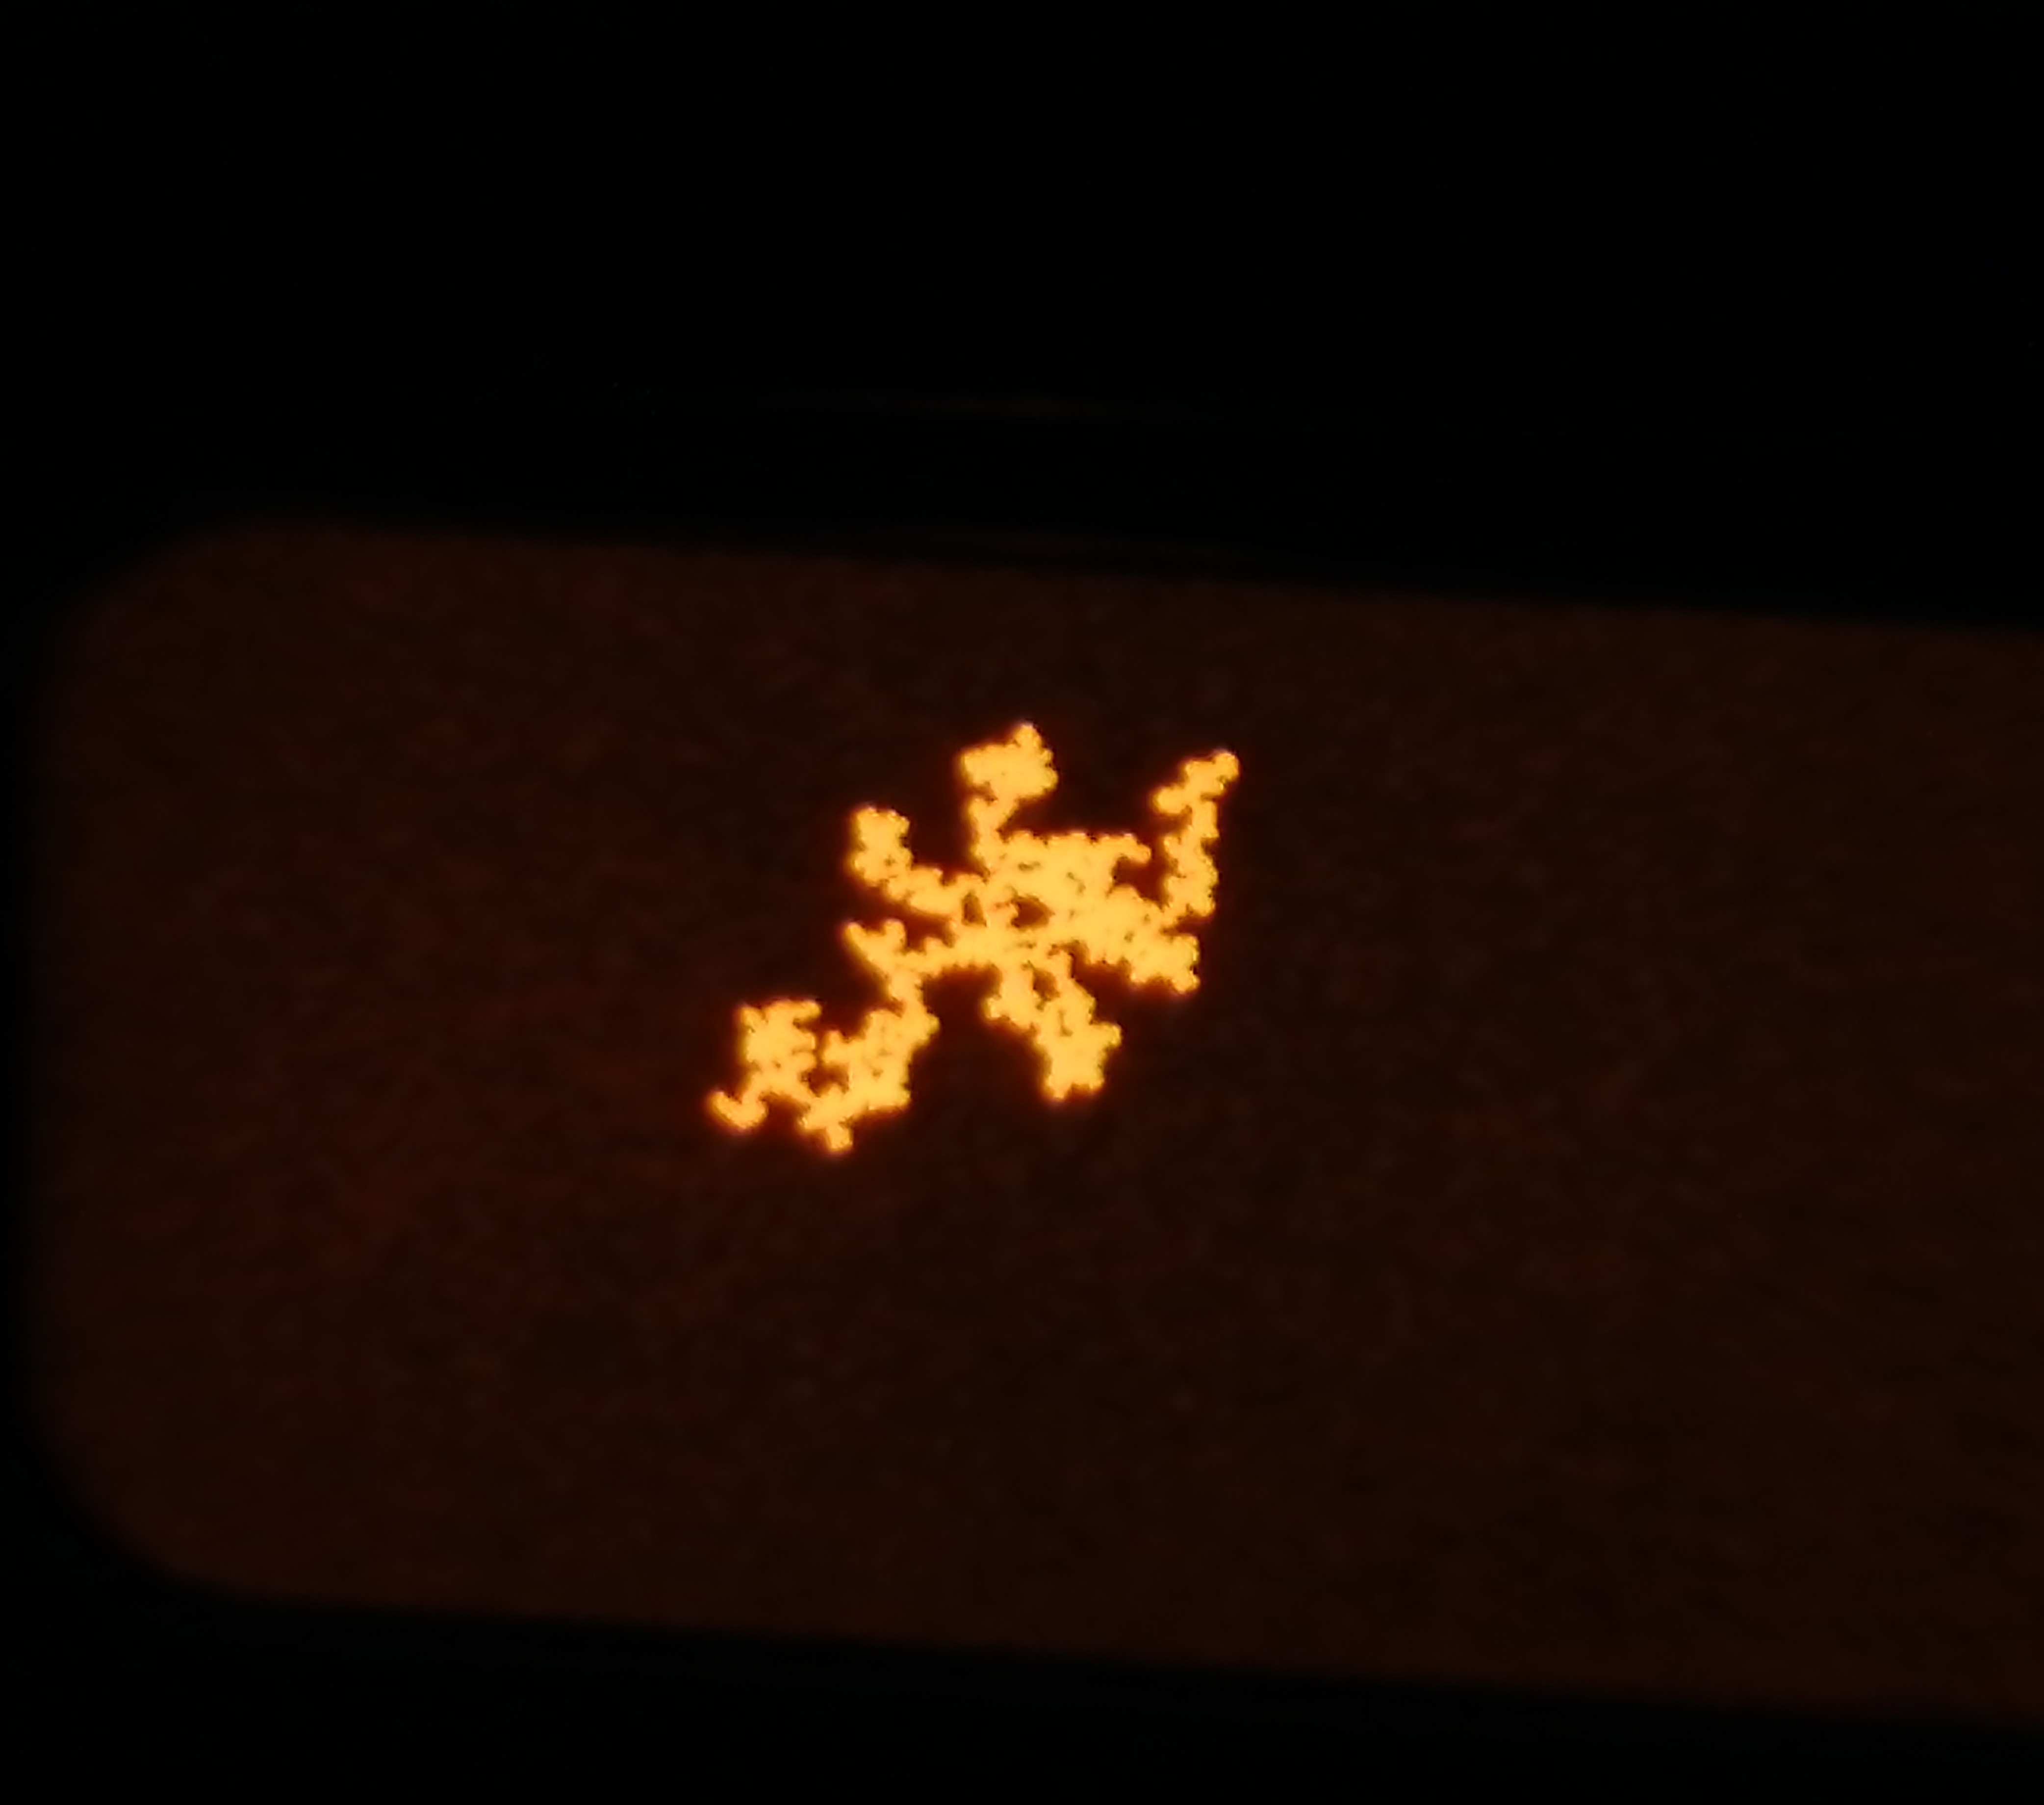
\includegraphics[height=5cm]{images/display.jpg}}
		\caption{light on} 
	\end{subfigure}
	\begin{subfigure}[b]{.47\textwidth}
		\centerline{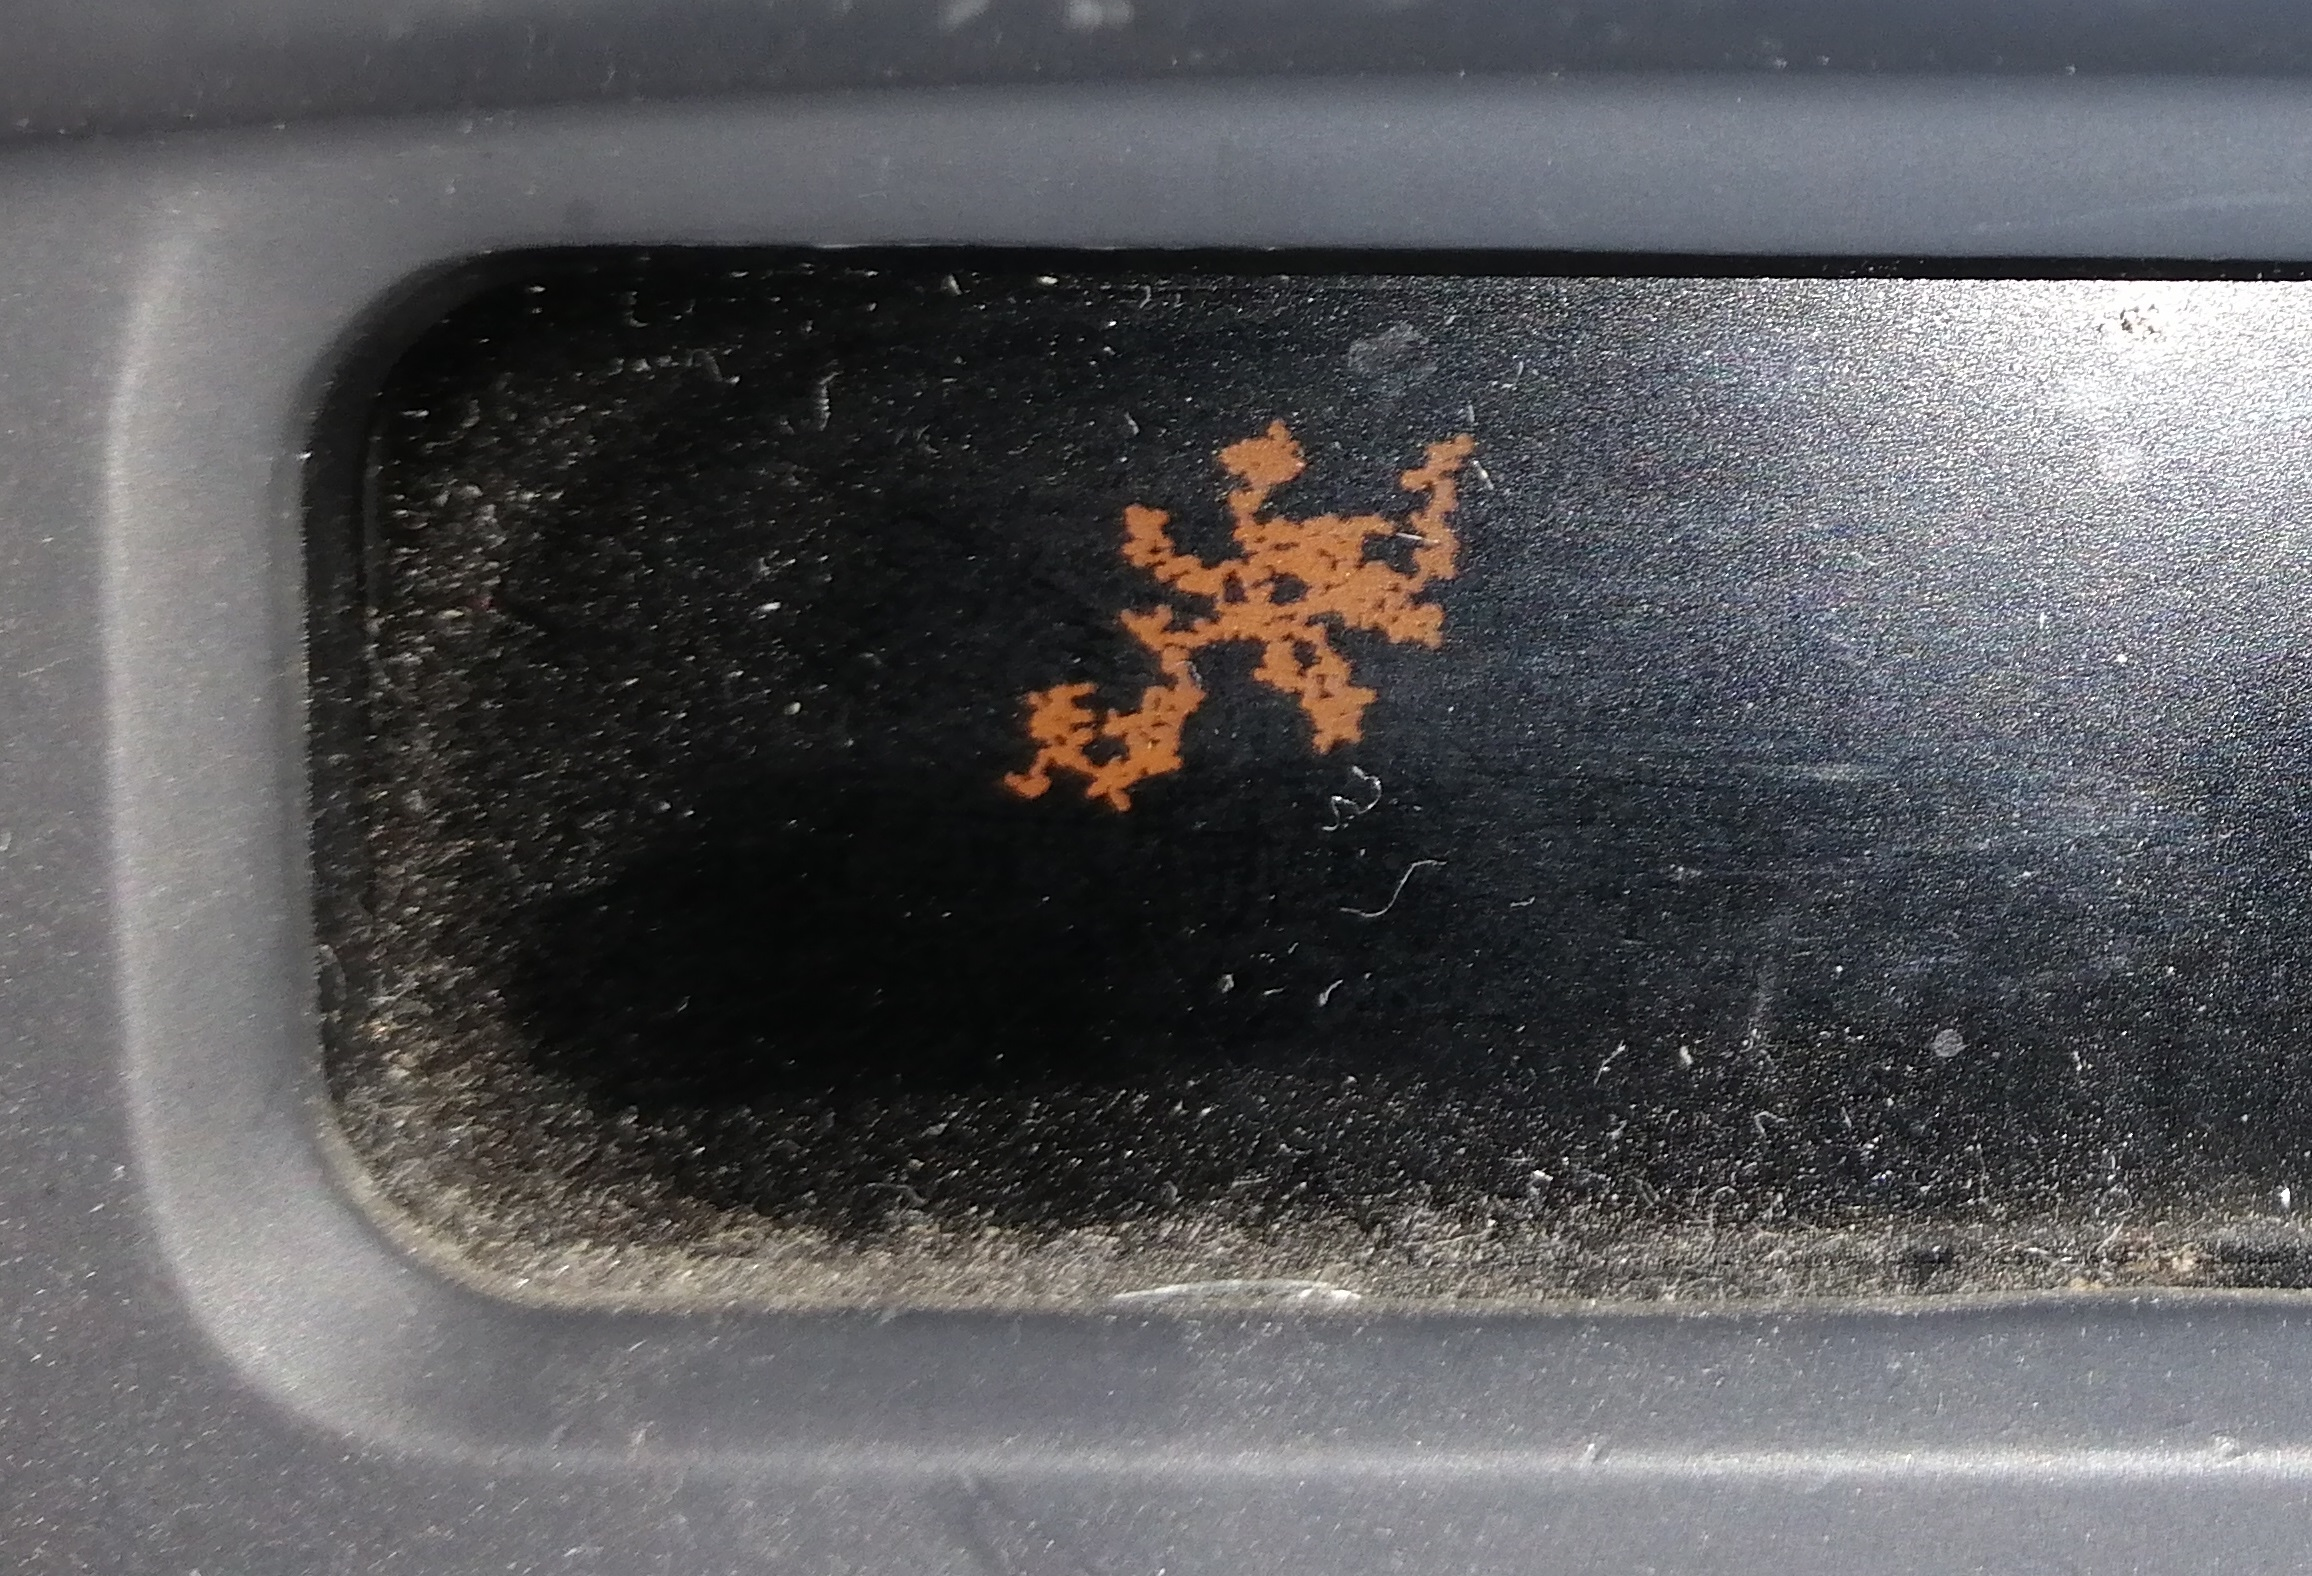
\includegraphics[height=5cm]{images/display2.jpg}}
		\caption{light off} 
	\end{subfigure}
	\caption{Cluster appearance in the radio screen of a car, \cite{own}}
	\label{radio}
\end{figure}

\vspace*{\fill}

\begin{figure}[h!]
	\centering
	\begin{subfigure}[b]{.45\textwidth}
		\centerline{
\includegraphics[height=5cm]{images/snowflake.png}}
		\caption{Snowflake crystals} 
	\end{subfigure}
	\begin{subfigure}[b]{.52\textwidth}
		\centerline{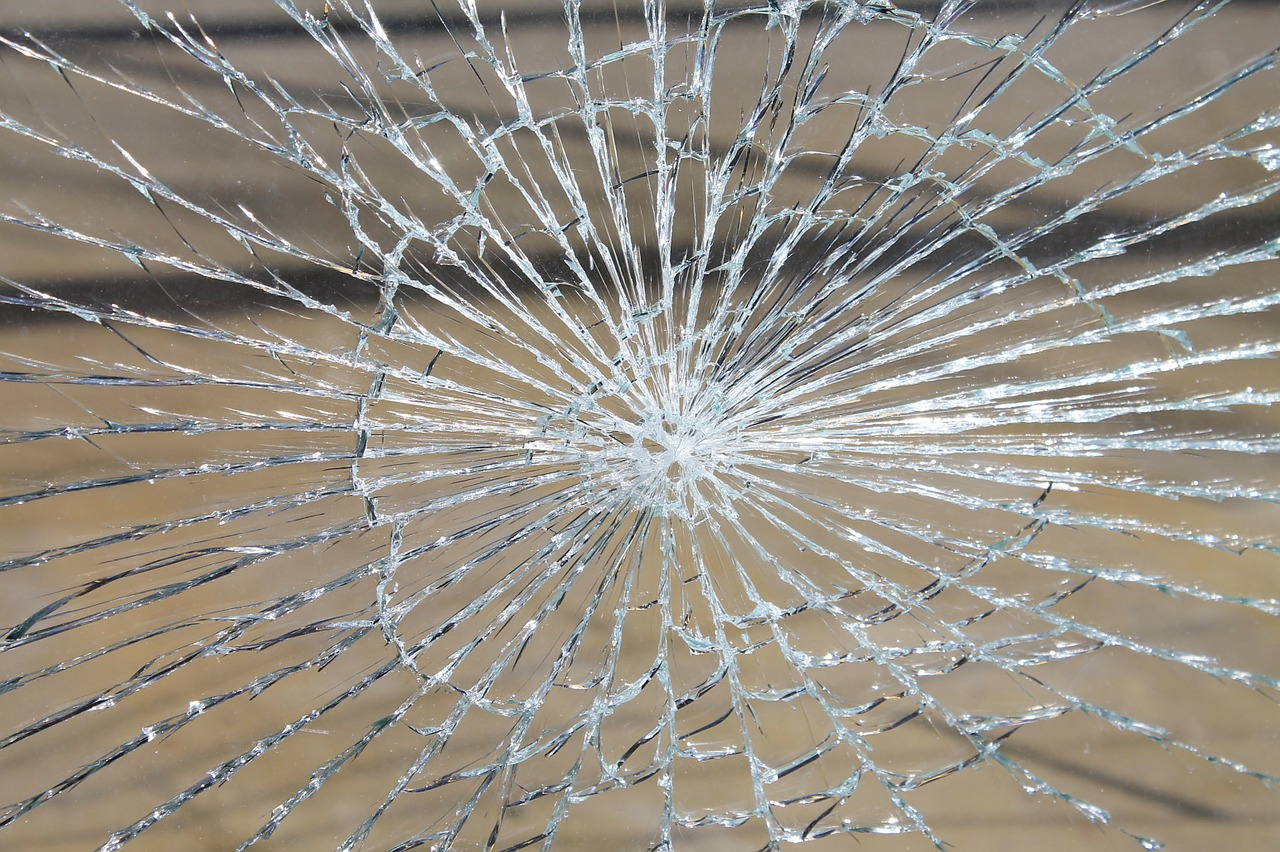
\includegraphics[height=5cm]{images/glass-break.jpg}}
		\caption{Cracked glass} 
	\end{subfigure}
	\caption{More examples of clusterlike formations, \cite{unsplash}}
	\label{other}
\end{figure}


\section{Preliminaries} \label{prelim}

\subsection{Symbols} \label{symbols}
Define the natural numbers $\N = \{1,2,3,\dots\}$, let $d\in \N$ and $q\in \{0,\dots,d\}$. 

\begin{longtable}{p{3.8cm}p{12.4cm}ll}
	$\mathcal{B}^d$ & $d$-dimensional Borel-$\sigma$-algebra of $\R^d$\\
	$\K^d$ & the set of convex and compact sets in $\R^d$\\
	$B_d(x,r)$ & $B_d(x,r) = \{y\in \R^d\ |\ |x-y| \leq r\}$, the $d$-dimensional closed ball of radius $r$ around $x$\\
	$B_r$ & $B_r := B_2(0,r)$\\
	$\G$ & the set of lines in the plane\\
	$SO_d$ & $SO_d := \{\nu \in \R^{d\times d}\ |\ \nu \nu^\top = I_d \text{ and } \det \nu = 1\}$\\
	$SO_2$ & $SO_2 := \{\nu_\beta := e^{i\beta} \in \C\ |\ \beta\in [0,2\pi)\}$\\
	$G_d$ & $G_d := \{\varphi: \R^d \to \R^d, x\mapsto \nu x+b\ |\ \nu \in SO_d\text{ and }b\in \R^d\}$, the set of Euclidean motions\\
	$\mP^d_f$ & the set of finite subsets of $\Z^d$\\
	$\mP_f$ & $\mP_f := \mP^2_f$
\end{longtable}

\noindent Note that we will always identify $\R^2$ with $\C$ ($(a,b)\leftrightarrow a+bi$) for a more convenient notation. 

\subsection{Expressions}

Throughout the paper let  $(\Omega,\mathcal{F}, \mathbb{P})$ be a probability space. If for $A\in \mathcal{F}$ we have $\mathbb{P}(A)=1$ we will say that \glqq $A \text{ holds }\mathbb{P}\text{-a.s.}$\grqq, or short \glqq$ A\text{ holds } \text{a.s.}$\grqq\ ($A$ holds almost surely). Another short expression we will use is that if for a set of logical statements $(A_t)_{t\in I}$ with $I\in\{\N,\R\}$ we say \glqq $A_t$ holds for large $t$\grqq\ it shall mean that there exists a $T\in I$ such that $A_t$ holds for all $t>T$. Here we mean that a logical statement holds if and only if the statement is true. 


\subsection{Graphs} \label{zgraph}

Let $d\in \N$. We will be interested in the undirected graph $(\Z^d, E)$ with its canonical graph structure, which is two vertices (or points) $x=(x_1,\dots,x_d),y=(y_1,\dots,y_d)\in \Z^d$ form an edge (e.q. $\{x,y\}\in E$) if and only if there exists exactly one $i\in \{1,\dots, d\}$ such that $|x_i - y_i| = 1$ and $x_j = y_j$ for all $j\neq i$. For a point $x\in \Z^d$ its set of $\mathit{neighbours}$ is defined as 
\begin{align*}
	N(x) := \{y\in \Z^d\ |\ \{x,y\}\in E\}.
\end{align*}
For a set $A\subset \Z^d$ the $\mathit{outer\ boundary}\ \partial A$ of $A$ is defined as 
\begin{align*}
	\partial A := \{y\in \Z^d\setminus A\ |\ \exists x\in A:\ \{x,y\}	\in E\}
\end{align*}
and the closure $\bar A$ of $A$ as 
\begin{flalign*}
	\bar A := A\cup \partial A.
\end{flalign*}
Instead of $(\Z^d, E)$ we will write $\Z^d$ from now on. 

\subsection{Random walks}

\begin{definition}
	 For our space of interest $\Z^d$ we will always use the discrete $\sigma$-algebra which is the power set of $\Z^d$. A family $(S_n)_{n\in \mathbb{N}_0}$ of measurable functions $S_n: \Omega \to \Z^d$ is called a $\mathit{random\ walk\ on}\ \Z^d$ $\mathit{(starting\ at}\ x\in \Z^d)$ if and only if $S_0=x$ a.s. and 
	
	\begin{align*}
		\mathbb{P}(S_n = y\ |\ S_{n-1} = z) = \frac{1}{|N(z)|} = \frac{1}{2d},\quad \text{ for all }  y\in N(z) \text{ and } z\in \Z^d.
	\end{align*}
	
	\noindent Note that $|N(z)| = 2d$ for all $z\in \Z^d$ since every point has two neighbours in the direction of every dimensional component. We can therefore conclude easily that $\mathbb{P}(S_n = y\ |\ S_{n-1} = z) = 0$ for all $y\notin N(z)$ and $z\in \Z^d$. For $x,y\in\Z^d$ we introduce the short notation
	\begin{flalign*}
		\PP_x(S_n=y) := \PP(S_n = y\ |\ S_0 = x). 
	\end{flalign*}
	
\end{definition}
So a random walk can be understood as a particle starting from some point $x$ and moving randomly on the grid choosing its next step uniformly from its neighbours. For the following let $(S_n)_{n\in \mathbb{N}}$ be a random walk on $\Z^d$ starting at $x\in \Z^d$. 

\begin{definition}
	Let $A\subset \Z^d$. We define the $hitting\ times$ of A by
	\begin{flalign*}
		T_A := \min \{n\geq 0\ |\ S_n\in A\}\text{ and } T^+_A := \min \{n\geq 1\ |\ S_n\in A\}, 
	\end{flalign*}
	and $T_y:= T_{\{y\}}$ and $T^+_y:= T^+_{\{y\}}$ for $y\in \Z^d$. We allow $T_A=\infty$ and $T_A^+=\infty$ if $A$ never gets hit. 
\end{definition}

\begin{definition}
	A random walk with origin in $x\in\Z^d$ is called  $\mathit{recurrent}$ if
	\begin{flalign*}
		\PP_x(T^+_x<\infty) = 1
	\end{flalign*}
	and $\mathit{transient}$ if
	\begin{flalign*}
		\PP_x(T^+_x<\infty) < 1.
	\end{flalign*}
\end{definition}

\begin{lemma} \label{recurr}
	A random walk on $\Z^d$ is recurrent if $d\leq 2$ and transient if $d\geq 3$. 
\end{lemma}
\begin{proof}
	Proofs of this result are presented in \cite[Satz 5.1]{henze} or \cite[Korollar 2.6.6]{markov}. 
\end{proof}

\begin{lemma} \label{recurrA}
	The following two statements are equivalent:
	\begin{enumerate}
		\item $\PP_x(T_x^+<\infty) = 1 \text{ for all } x\in\Z^2$
		\item $\PP_x(T_A^+<\infty) = 1 \text{ for all } x\in\Z^2 \text{ and } A\subset\Z^2$
	\end{enumerate}
\end{lemma}

\begin{proof}
	The direction $(ii)$ to $(i)$ is clear. For the other direction choose $x\in\Z^2$ and $A\subset \Z^2$. We know that in general for any point $y\in\Z^2$ we have $\PP_x(T_y^+<\infty) > 0$ for a random walk in $\Z^d$ for any dimension $d\in\N$. By Lemma \ref{recurr} we know that a random walk on $\Z^2$ is recurrent. For that case it is proved  in \cite[Satz 2.6.9]{markov} that for $y\in\Z^2$ even $\PP_x(T_y^+<\infty) = 1$ holds. If we choose $y\in A$ we get
	\begin{flalign*}
		1 = \PP_x(T_y^+<\infty) \leq \PP_x(T_A^+<\infty),
	\end{flalign*}
	which completes the proof. 
\end{proof}

After having introduced some basics we will turn our focus in the next chapter to the main definition of stochastic processes we will discuss in this paper. 


\newpage
\phantom \\
\newpage
\section{Incremental aggregation}

\subsection{Definition} \label{iadef}

In this paper we will look at stochastic processes on the set of finite subsets of $\Z^d$, where we start with the one point set $\{0\}$ and incrementally add a point of the boundary of the current cluster according to some distribution. Note that with $0$ we denote the zero vector $(0,\dots,0)$. What we get is a randomly point by point growing connected cluster which we will call $\mathit{incremental\ aggregation}$. Define 
\begin{flalign*}
	\mP^d_f := \{A\subset \Z^d\ |\ \text{A is finite}\}
\end{flalign*}
the set of finite subsets of $\Z^d$. Furthermore we will be interested in distributions on those sets, so for $A\in \mP^d_f$ we define 
\begin{flalign*}
	\mathcal{D}_A:= \{\mu: \Z^d\to [0,1]\ |\ \mu(y) = 0 \text{ for all } y\notin A\ \text{and}\ \sum_{y\in A} \mu(y) = 1 \}
\end{flalign*}
the set of distributions on $A$. For $\mP^d_f$ we consider the discrete $\sigma$-algebra and call a measurable function
\begin{flalign*}
	F:\Omega\to \mP^d_f
\end{flalign*}
a $\mathit{random}$ $\mathit{finite\ set}$. Further for $A\in\mP^d_f$ we call a measurable function
\begin{flalign*}
	y_A:\Omega\to \Z^d
\end{flalign*}
a $\mathit{random}$ $\mathit{point}$ $\mathit{in\ A}$ if $\PP(y_A = y) = 0$ is satisfied for all $y\notin A$. Now we define incremental aggregation as follows.  

\begin{definition} \label{incrementalaggregation}
	Let $\mu:=(\mu_A)_{A\in \mP^d_f}$ be a family of distributions, therefore $\mu_A\in \mathcal{D}_A$ for all $A\in \mP^d_f$. An $\mathit{incremental\ aggregation\ (with\ distribution\ \mu)}$ is a family of random finite sets $(\mathcal{E}_n)_{n\in{\mathbb{N}}}$ which evolves as follows. The process starts with one point $\mathcal{E}_1 = \{0\}$ (define $y_1 :=0$) at the origin of $\Z^d$. Knowing the process $\mathcal{E}_n$ at time $n$, let $y_{n+1}$ be a random point in $\partial \mathcal{E}_n\in \mP^d_f$ with distribution
	\begin{align}
		\mathbb{P}(y_{n+1} = y\ |\ \mathcal{E}_n) := \mu_{\partial \mathcal{E}_n}(y)\quad \text{for }y\in \Z^d.
	\end{align}
	We then define $\mathcal{E}_{n+1} := \mathcal{E}_n \cup \{y_{n+1}\}$ and the limit cluster as $\E_\infty := \bigcup_{n\in\N} \E_n$. This naturally defines a Markov chain. 
\end{definition} 

\begin{remark}
	We want to quickly argument here that all $\E_n$ are indeed measurable functions. $\E_1 = \{0\}$ is constant and therefore measurable. It is not difficult to show that for $A\in\mP^d_f$ we have
	\begin{flalign*}
		\E_{n+1}^{-1}(A) = \bigcup_{y\in A} \E_n^{-1}(A\setminus \{y\}) \cap y_{n+1}^{-1}(\{y\})
	\end{flalign*}
	for any $n\in\N$ and we can therefore conclude the measurability for all $\E_n$ by induction. 
\end{remark}

\begin{remark} \label{orderindependence}
	It is worth to mention that since incremental aggregations are Markov chains the distribution of a new added point $y_{n+1}$ is not depending on the order of how previous points where added to the cluster.
\end{remark}

Properties of an incremental aggregation obviously base strongly on the properties of its distribution $\mu$. In the following we prepare some additional definitions which we will use later on. 

\begin{definition} \label{outsidedist}
	We call a distribution family $(\mu_A)_{A\in \mP^d_f}$ an $\mathit{outside\ distribution}$ if and only if for all connected sets $A\in\mP^d_f$ we have that 
	\begin{flalign*}
		\mu_{\bar A} (x) = 
		\begin{cases}
			\mu_{\partial A}(x), \quad &x\in\partial A, \\
			0, \quad &x\in A.
		\end{cases}
	\end{flalign*}
	Recall that $\bar A = A \cup \partial A$. This definition shall capture the idea that particles coming from \glqq outside\grqq\ to a set $\bar A$ shall not be able to move into the \glqq inside\grqq\ $A$ of that set without passing its boundary $\partial A$ first. For both incremental aggregations we discuss in this paper this will be the case. 
\end{definition}

\begin{definition} \label{translinv}
	For $y\in\Z^d$ let 
	\begin{flalign*}
		\Phi_y: \Z^d \to \Z^d, x\mapsto x+y
	\end{flalign*}
	be a translation function on $\Z^d$. Then we call the family of distributions $(\mu_A)_{A\in\mP^d_f}$ $\mathit{translation}$ $\mathit{invariant}$ if and only if for all $y\in\Z^d$
	\begin{flalign*}
		\mu_A(z) = \mu_{\Phi_y(A)}(\Phi_y(z)) 
	\end{flalign*}
	for all $z\in A$ and $A\in\mP^d_f$. 
\end{definition}

As a last result before coming to the next section we want to prove an useful result here. 

\begin{proposition} \label{limexists}
	For each $\omega\in\Omega$ the limit
	\begin{flalign*}
		\lim_{n\to\infty} \frac{\ln(n)}{\ln(\rad(\E_n(\omega)))}
	\end{flalign*}
	exists. 
\end{proposition}

\begin{proof}
	Let $\omega\in\Omega$, define $r_n := \rad(\E_n(\omega))$ for all $n\in\N$ and let $N\in\N$ such that $r_n>\sqrt{d}$ for all $n>N$ which exists by Lemma \ref{rtinfty}. For $n>N$ define
	\begin{flalign*}
		a_n := \frac{\ln(n)}{\ln(r_n)}.
	\end{flalign*}
	Further define
	\begin{flalign*}
		M := \{m>N\ |\ r_{m+1} > r_m\}
	\end{flalign*}
	and write $M=\{m_1, m_2, \dots\}$ with $m_i<m_j$ for $i<j$. By Lemma \ref{rtinfty} we know that $|M|=\infty$. For $i\in\N$ we further define
	\begin{flalign*}
		B_i := \frac{\ln(m_{i+1})}{\ln(r_{m_{i+1}})}
	\end{flalign*}
	and
	\begin{flalign*}
		C_i := \frac{\ln(m_i)}{\ln(r_{m_i}) + \ln(2)}. 
	\end{flalign*}
	Let $i\in\N$ and $n\in\{m_i + 1,\dots,m_{i+1}\}$. Note that on $\{m_i + 1,\dots,m_{i+1}\}$ the sequence $(a_n)$ is increasing since its denominator $\ln(r_n)$ is constant on that set. We therefore get
	\begin{flalign*}
		a_n \leq B_i
	\end{flalign*}
	and 
	\begin{flalign*}
		a_n \geq \frac{\ln(m_i + 1)}{\ln(r_{m_i + 1})} \geq  \frac{\ln(m_i)}{\ln(r_{m_i} + \sqrt{d})} \geq \frac{\ln(m_i)}{\ln(2r_{m_i})} = C_i. 
	\end{flalign*}
	We used here that $r_{m_i + 1}\leq r_{m_i} + \sqrt{d}$ since adding one particle can increase the radius maximally by the diagonal of a $d$-dimensional box which is $\sqrt{d}$. Since $m_i>N$ we also used that $r_{m_i}>\sqrt{d}$ by definition of $N$. If we define sequences $(b_n)_{n>m_1}$ and $(c_n)_{n>m_1}$ by
	\begin{flalign*}
		b_n := \sum_{i=1}^{\infty} B_i\ \1_{\{m_i + 1,\dots,m_{i+1}\}}(n)
	\end{flalign*}
	and
	\begin{flalign*}
		c_n := \sum_{i=1}^{\infty} C_i\ \1_{\{m_i + 1,\dots,m_{i+1}\}}(n)
	\end{flalign*}
	for $n>m_1$, then we simply get that
	\begin{flalign*}
		c_n \leq a_n \leq b_n
	\end{flalign*}
	for all $n>m_1$. Note that 
	\begin{flalign*}
		\limsup_{n\to\infty} b_n = \limsup_{i\to\infty} B_i
	\end{flalign*}
	and
	\begin{flalign*}
		\limsup_{n\to\infty} c_n = \limsup_{i\to\infty} C_i.
	\end{flalign*}
	Since $(B_i)_{i\in\N}$ is a subsequence of $(a_n)_{n>N}$ and $a_n\leq b_n$ for all $n>m_1$, we get
	\begin{flalign*}
		\limsup_{n\to\infty} a_n = \limsup_{n\to\infty} b_n. 
	\end{flalign*}
	Since 
	\begin{flalign*}
		\frac{1}{B_i} \leq \frac{1}{C_{i+1}} = \frac{1}{B_i} + \frac{\ln(2)}{\ln(m_i)}
	\end{flalign*}
	for all $i\in\N$ by definition of $B_i$ and $C_i$, we also get that
	\begin{flalign*}
		\limsup_{n\to\infty} c_n = \limsup_{i\to\infty} C_i = \liminf_{i\to\infty} \frac{1}{C_i} = \liminf_{i\to\infty} \frac{1}{B_i} = \limsup_{i\to\infty} B_i = \limsup_{n\to\infty} a_n.
	\end{flalign*}
	But since $a_n\geq c_n$ for all $n>m_1$ we get that 
	\begin{flalign*}
		\liminf_{n\to\infty} a_n \geq \limsup_{n\to\infty} c_n = \limsup_{n\to\infty} a_n
	\end{flalign*}
	and therefore 
	\begin{flalign*}
		\liminf_{n\to\infty} a_n = \limsup_{n\to\infty} a_n. 
	\end{flalign*}
	In $\Z^d$ we can fill the cube with center $0$ and side length $n^{\frac{1}{d}}$ with an order of $n$ points. Therefore we can fill a ball with radius $n^{\frac{1}{d}}$ with an order of $n$ points as well, and since $|\E_n(\omega)|=n$ there exists a constant $c>0$ such that $cn^{\frac{1}{d}} \leq \rad(\E_n(\omega))$. Note that $c$ does not depend on $n$ or $\omega$. Hence
	\begin{flalign*}
		\limsup_{n\to\infty} a_n \leq \limsup_{n\to\infty} \frac{\ln(n)}{\ln(cn^{\frac{1}{d}})} = d.
	\end{flalign*}
	Therefore $\limsup_{n\to\infty} a_n <\infty$ which completes the proof.
\end{proof}

\begin{remark} \label{trivialboundary2}
	We quickly show some trivial bounds for the limit of the last theorem. Let $\omega\in\Omega$ and define 
	\begin{flalign*}
		L := \lim_{n\to\infty} \frac{\ln(n)}{\ln(\rad(\E_n(\omega)))}.
	\end{flalign*}
	Then since $\rad(\E_n(\omega))\leq n$ we get
	\begin{flalign*}
		L \geq \lim_{n\to\infty} \frac{\ln(n)}{\ln(n)} = 1.
	\end{flalign*}
	By an argument we can find in the proof of Proposition \ref{limexists} we get that 
	\begin{flalign*}
		L \leq  d,
	\end{flalign*}
	leading to the trivial bounds
	\begin{flalign*}
		1\leq L \leq d.
	\end{flalign*}
\end{remark}


\subsection{Notion of fractal dimension and growth rate} \label{notion}

\begin{figure}
	\centering
	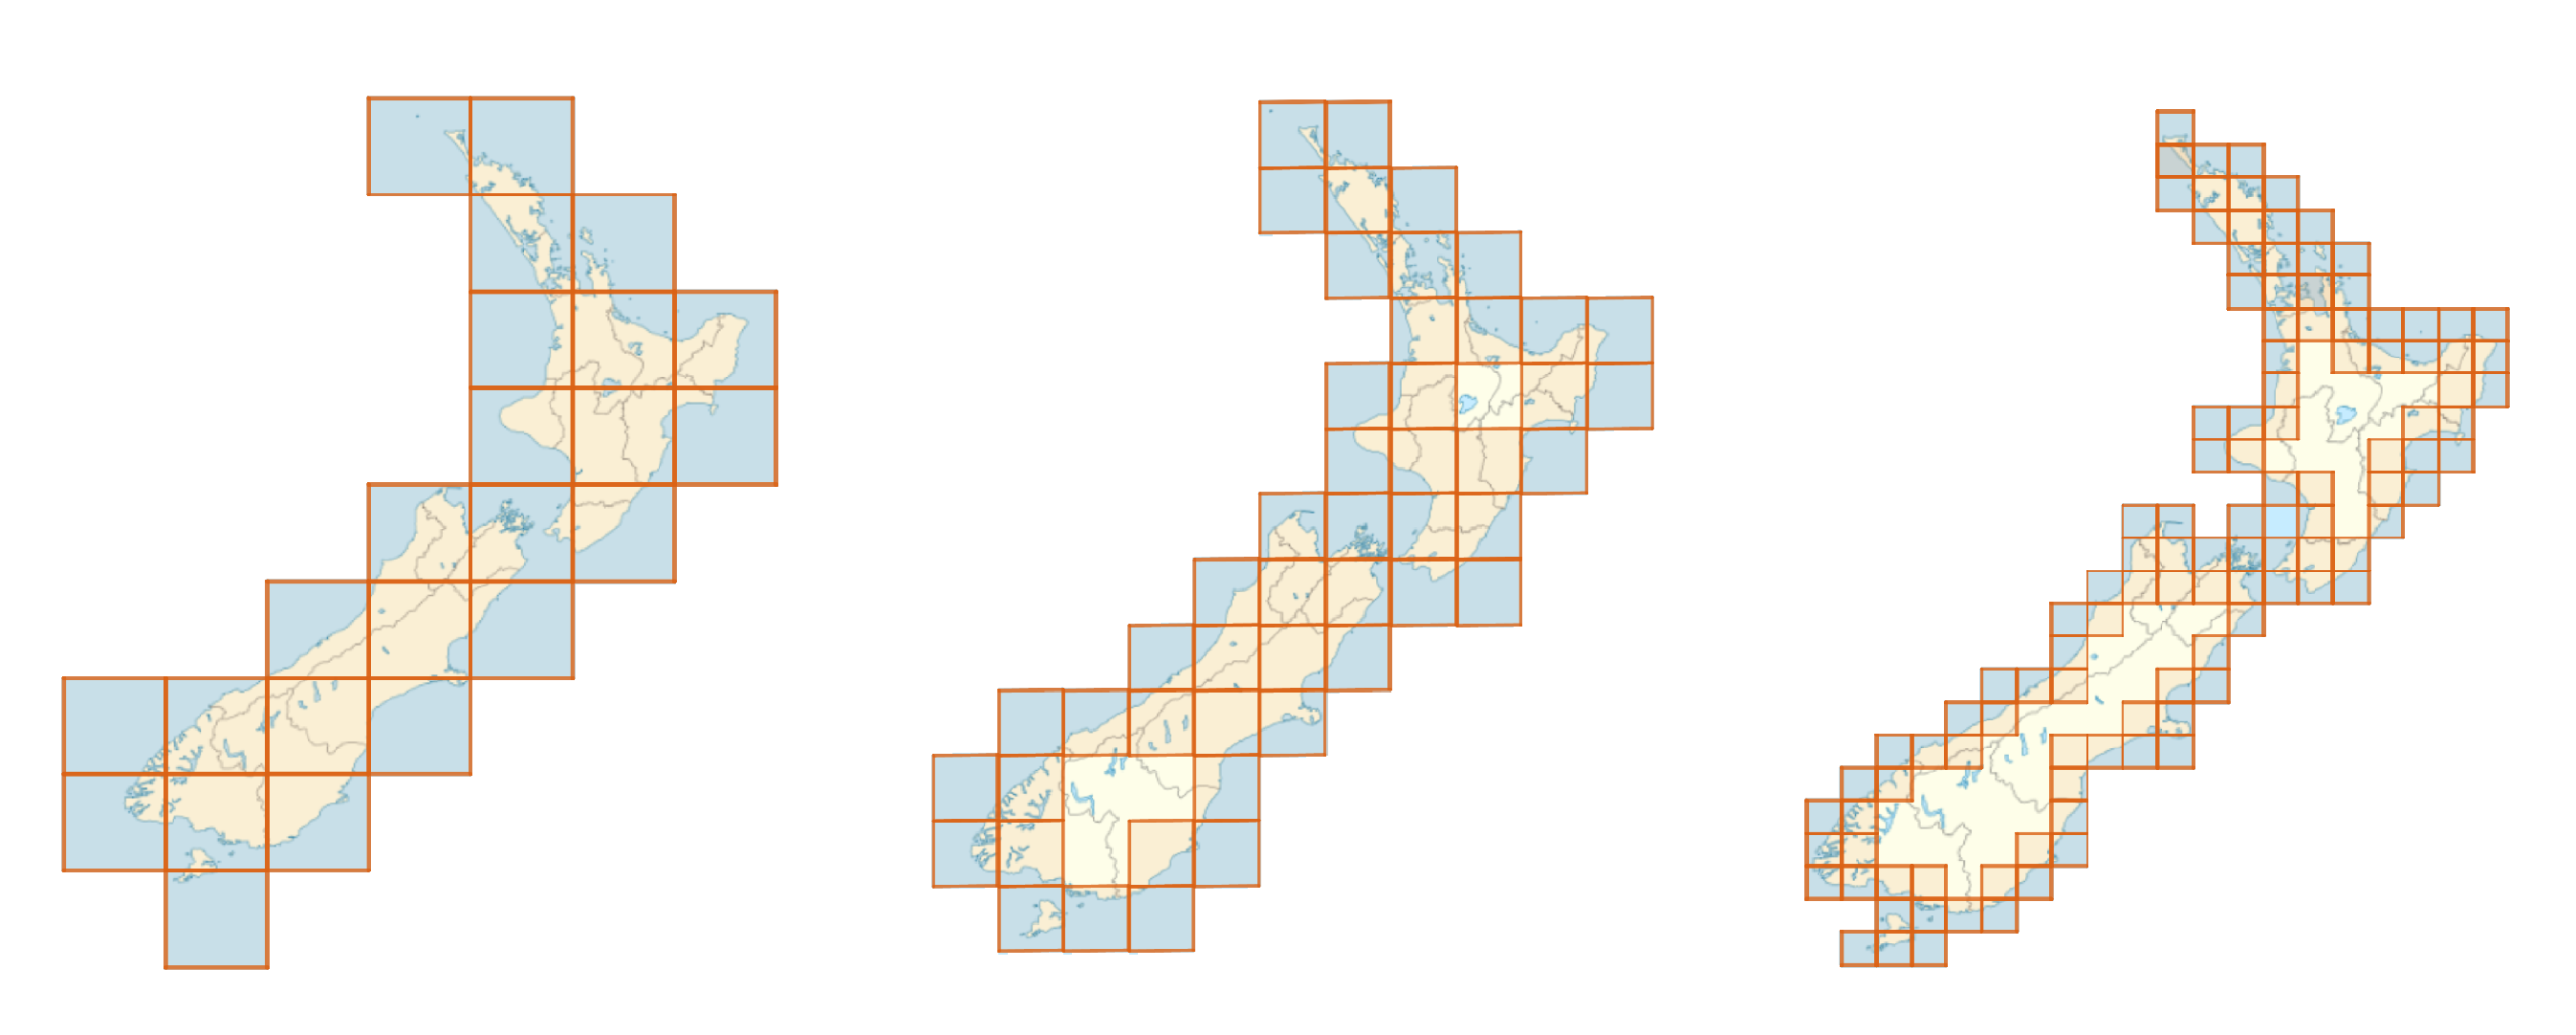
\includegraphics[height=6.5cm]{images/geogebra-images/neuseeland-squares.png}
	\caption{Box-covering of New Zealands outer cost with decreasing box sizes $\varepsilon$} \label{neuseeland}
\end{figure}

The notion of fractal dimension is usually used for sets with uncountable cardinality like continuous curves or surfaces. One way of defining a fractal dimension for curves like for example the coast line of New Zealand (see \autoref{neuseeland}) would be to look at the asymptotic relation between the minimal number of grid boxes (squares) which we need to cover the cost line and the side length of these boxes. The following definition is motivated by \cite[Page 160]{hausdorff}. If, for $\varepsilon>0$, $N(\varepsilon)$ is the mininum number of boxes with side length $\varepsilon$ which we need to cover the coast line, then the so called $\mathit{box\ dimension\ d_b}$ is roughly the constant such that $N(\varepsilon)$ grows like $\varepsilon^{-d_b}$ as $\varepsilon$ tends to zero, so 
\begin{flalign} \label{boxdimension}
	d_b := - \liminf_{\varepsilon\to 0} \frac{\ln(N(\varepsilon))}{\ln(\varepsilon)}.
\end{flalign} 
This definition makes sense in many contexts, for example the box-dimension of straight line segments is $1$ and of squares is $2$ and so on, so in those cases equal to the topological dimension. As with incremental aggregations we are dealing with locally finite point sets, this approach of defining a fractal dimension for our clusters is not senseful. It is not difficult to show, that the box-dimension of any finite set is $0$. A helpful detail about the situation with finite sets as the ones we are looking at, is that each point of the cluster can actually be interpreted and identified with a unique box of side length 1 since the cluster is living on the grid $\Z^d$. We will precise that in Chapter \ref{lha}. So instead of decreasing the sizes of the boxes which we cover our set of interest with, we leave the size of the boxes constant and increase the size of our set by adding points and looking at the limit cluster $\E_\infty$. 
Defining the radius of a finite set $A\in \mP^d_f$ (with $|\cdot|$ the Euclidean norm) by 
\begin{flalign} \label{radius}
	\rad(A) := \max_{x\in A} |x|,
\end{flalign}
we can identify the relation between the geometrical sizes of the boxes and the cluster as follows. For $n\in\N$ define random variables  $\varepsilon_n:=\frac{1}{\rad(\E_n)}$. Before $\varepsilon_n$ would have expressed the geometrical relation between one box and the whole cluster which we describe now by the fraction $\frac{1}{\rad(\E_n)}$ since a box size is now constantly $1$ and the clusters geometrical size we can interpret by $\rad(\E_n)$. The number of boxes with size $1$ which we need to cover $\E_n$ is always $n$, so $N(\varepsilon_n)=n$ for all $n\in\N$ and therefore we can rewrite the definition of the box-dimension (\ref{boxdimension}) by replacing $\varepsilon_n$ with $\frac{1}{\rad(\E_n)}$ and define the $\mathit{(discrete)\ fractal\ dimension}$ of $\E_\infty$ as the random variable 
\begin{flalign} \label{fractaldimension}
	d_f := \lim_{n\to\infty} \frac{\ln(n)}{\ln(\rad(\E_n))},
\end{flalign}
which is well-defined by Proposition \ref{limexists}. This way of defining a fractal dimension for incremental aggregations strongly correlates with the growth rate of the aggregation which shall indicate how the radius of the cluster evolves while increasing the particle number. We can define the growth rate by looking for the smallest exponent $\alpha$ such that there exists a constant $c>0$ with 
\begin{flalign*}
	\rad(\E_n) \leq cn^\alpha
\end{flalign*}
for large $n$. Rewriting this we come to the equivalent inequality
\begin{flalign*}
	\frac{\ln(\rad(\E_n))}{\ln(n)} - \frac{\ln(c)}{\ln(n)} \leq \alpha
\end{flalign*}
for large $n$ and we could finally define the growth rate $\alpha_f$ of an incremental aggregation as the smallest value satisfying this inequality, so the random variable
\begin{flalign} \label{growthrate}
	\alpha_f := \lim_{n\to\infty} \frac{\ln(\rad(\E_n))}{\ln(n)}
\end{flalign}
which is aswell well-defined by Proposition \ref{limexists}. We therefore simply get
\begin{flalign} \label{fractaldim}
	d_f = \frac{1}{\alpha_f},\quad\text{pointwise}. 
\end{flalign}
In Remark \ref{trivialboundary2} we have shown trivial bounds for the fractal dimension
\begin{flalign}
	1\leq d_f \leq d,\quad\text{pointwise},
\end{flalign}
which leads to trivial bounds for the growth rate
\begin{flalign*}
	\frac{1}{d}\leq \alpha_f \leq 1,\quad\text{pointwise},
\end{flalign*}
for any incremental aggregation in $\Z^d$. 


\begin{remark} \label{altdim}
	Another way of tackling the intuition for a fractal dimension for locally finite sets is the following which is motivated by \cite[Section 1.3, Page 2]{heydenreich} and \cite[Page 83]{lawler}. Let $M\subset \R^d$ be a locally finite set. Let $n\in\N$ and $B_n$ be the ball with radius $n$ and center $0$. We could interpret the fractal dimension $d_M$ of $M$ as a value such that the cardinality $|M\cap B_n|$ of $M$ inside the ball $B_n$ is rougly of order $n^{d_M}$ for large $n$, so 
	\begin{flalign} \label{newdef}
		d_M := \liminf_{n\to\infty} \frac{\ln(|M \cap B_n|)}{\ln(n)}. 
	\end{flalign}
	If we apply that definition to our limit cluster $\E_\infty$ it is not clear whether this definition is equivalent to (\ref{fractaldimension}). If we define the fractal dimension as in (\ref{fractaldimension}) we encounter the problem that when the cluster reaches some radius for the first time, then in many instances in the subsequent steps there will particles be added to the cluster without increasing its radius, so to say \glqq $\text{filling}$\grqq\ the cluster up to that radius (see \autoref{notfilled}). If the fractal dimension shall indicate an asymptotic relation between how many particles of the limit cluster $\E_\infty$ lie in a ball of a radius letting the radius tend to infinity, the definition in (\ref{fractaldimension}) does not reflect that directly. In the following we give an alternative definition for the fractal dimension.
\end{remark}

\begin{definition} \label{fullclusters}
	Let $B_n$ be a ball of radius $n\in\N$ with center $0$ and with $\E_\infty \cap B_n$ denote the set of particles in $\E_\infty$ that lie in $B_n$. We define
	\begin{flalign*}
		\underline{d}_\infty := \liminf_{n\to\infty} \frac{\ln(|\E_\infty \cap B_n|)}{\ln(n)},
	\end{flalign*}
	\begin{flalign*}
		\overline{d}_\infty := \limsup_{n\to\infty} \frac{\ln(|\E_\infty \cap B_n|)}{\ln(n)}
	\end{flalign*}
	and 
	\begin{flalign*}
		d_\infty := \lim_{n\to\infty} \frac{\ln(|\E_\infty \cap B_n|)}{\ln(n)},
	\end{flalign*}
	if the limit exists. Similar to $d_f$ we have trivial bounds
	\begin{flalign*}
		1 \leq \underline{d}_\infty \leq \overline{d}_\infty \leq d,\quad\text{pointwise}.
	\end{flalign*}
\end{definition}

As for $d_f$ in Proposition \ref{limexists} it might be possible to show that the limit $d_\infty$ indeed exists. It seems to make sense that these two situations are equivalent if the distribution family $\mu$ doesn't favorize outer lying particles for the next aggregation too much. If it does, the creation of long arms would become more probable increasing the difference between the definitions of $d_f$ and $d_\infty$. If it doesn't, arms will rather decrease in size compared to the size of the cluster which in turn closes the gap in between the definitions of $d_f$ and $d_\infty$. Anyway we find a rigorous inequality in the following. \\

\begin{lemma} \label{smaller}
	We have 
	\begin{flalign*}
		d_f \leq \underline{d}_\infty, \quad\text{pointwise}.
	\end{flalign*}
\end{lemma}

\begin{proof}
	Let $\omega\in\Omega$. Then for all $n\in\N$ we have $\E_n(\omega)\subset \E_\infty(\omega)$ and therefore
	\begin{flalign*}
		n=|\E_n(\omega)| \leq |\E_\infty(\omega) \cap B_{\rad(\E_n(\omega))}|.
	\end{flalign*}
	This leads to
	\begin{flalign*}
		d_f(\omega) &= \lim_{n\to\infty} \frac{\ln(n)}{\ln(\rad(\E_n(\omega)))} \leq \liminf_{n\to\infty} \frac{|\E_\infty(\omega) \cap B_{\rad(\E_n(\omega))}|}{\ln(\rad(\E_n(\omega)))} \\
		&= \liminf_{k\to\infty} \frac{|\E_\infty(\omega) \cap B_{k}|}{\ln(k)} = \underline{d}_\infty(\omega)
	\end{flalign*}
	where we used that for every $k\in\N$ there exists a $n\in\N$ such that $\rad(\E_n(\omega)) = k$. This completes the proof. 
\end{proof}

\begin{figure}[]
	\centering
	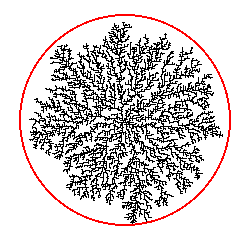
\includegraphics[height=6cm]{images/fractal_range/5.png}
	\caption{Cluster not \glqq filled up\grqq\ to its radius} \label{notfilled}
\end{figure}















\subsection{A rigorous result on the fractal dimension}

In this section we will proof an almost sure lower bound for the fractal dimension of an incremental aggregation if its distribution family $(\mu_A)_{A\in\mP^d_f}$ satisfies some conditions. Before coming to this statement we have to make some preparations in the following. We define two random functions
\begin{flalign*}
	r: \N \to [0,\infty),\quad n\mapsto \rad(\E_n)
\end{flalign*}
and
\begin{flalign*}
	T: [0,\infty) \to \N,\quad s\mapsto \min\{j\in\N\ |\ r(j)\geq s\}.
\end{flalign*}
Recall that $\rad(\E_n)$ is the radius of the cluster at time $n$ as defined in (\ref{radius}). 
\begin{remark}\label{props}
	It is easy to show that for all $\omega\in\Omega$ the functions $r(\omega)$ and $T(\omega)$ are increasing in $n\in\N$ resp. $s\in [0,\infty)$ and that for all $n\in\N$ and $s\in [0,\infty)$ we have $T(\omega)(r(\omega)(n)) \leq n$ and  $r(\omega)(T(\omega)(s)) \geq s$.
\end{remark}

\begin{lemma} \label{rtinfty}
	For both random functions $r$ and $T$ we have that
	\begin{flalign*}
		r(\omega)(n) \to\infty \text{ for } n\to\infty
	\end{flalign*}
	and
	\begin{flalign*}
		T(\omega)(s) \to\infty \text{ for } s\to\infty
	\end{flalign*}
	for all $\omega\in\Omega$.
\end{lemma}
\begin{proof}
	Since we are moving on the grid $\Z^d$ we have that for a ball $B_d(0,n)$ with radius $n\geq0$ the number $N:=|B_d(0,n)\cap \Z^d|$ is finite and for any $\omega\in\Omega$ we get 
	\begin{flalign*}
		r(\omega)(2N)\geq n. 
	\end{flalign*}
	Therefore for all $\omega\in\Omega$ and any $n\in\N$ we can find a $M\in\N$ such that $r(\omega)(M)\geq n$, and since $r(\omega)$ is increasing we get $r(\omega)(n) \to\infty \text{ for } n\to\infty$ for all $\omega\in\Omega$. Very similarly we can argue for $T$. 
\end{proof}

\begin{lemma} \label{randt}
	Let $a>0$ and $h:[0,\infty) \to [0,\infty)$ be a bijective, multiplicative and increasing function. For $c>0$ define
	\begin{flalign*}
		A_c:=\{\omega \in\Omega\ |\ \exists N=N(\omega)\in\N: r(\omega)(n) \leq ch(n) \text{ for all } n>N\}
	\end{flalign*}
	and
	\begin{flalign*}
		D_c := \{\omega \in\Omega\ |\ \exists N=N(\omega)\in\N: T(\omega)(as)\geq ch^{-1}(s) \text{ for all } s>N\}.
	\end{flalign*}
	Then the following are equivalent:
	\begin{enumerate}
		\item $\exists c>0: \PP(A_c) = 1$ 
		\item $\exists c>0: \PP(D_c)=1$
	\end{enumerate}
\end{lemma}

\begin{proof} 
	$\Rightarrow$: Choose $c>0$ such that $\PP(A_c)=1$. Take $\omega\in A_c$ and choose $N\in\N$ such that $r(\omega)(n)\leq ch(n)$ for all $n>N$. Hence there exists $\tilde c>0$ such that $\tilde ch^{-1}(r(\omega)(n))\leq n$ for all $n>N$. By Lemma \ref{rtinfty} we can choose $M\in\N$ big enough such that $T(\omega)(aM) > N$, hence $T(\omega)(as)\geq T(\omega)(aM) > N$ for all $s>M$ since $T(\omega)$ is increasing. Hence we can write $\tilde c h^{-1}(r(\omega)(T(\omega)(as))) \leq T(\omega)(as)$ for all $s>M$ and since $r(\omega)(T(\omega)(as))\leq as$ we finally get $\tilde c h^{-1}(a)h^{-1}(s)=\tilde ch^{-1}(as) \leq T(\omega)(as)$ for all $s>M$, hence $\omega \in D_{\tilde c h^{-1}(a)}$, where we used the multiplicativity of $h$ and that $h^{-1}$ is decreasing. We therefore get $A_c\subset D_{\tilde c h^{-1}(a)}$, hence $\PP(D_{\tilde c h^{-1}(a)}) = 1$.\\
	$\Leftarrow$: 
	The proof for this direction works analogously and needs Lemma \ref{rtinfty} as well.
\end{proof}

\begin{lemma} \label{geometric}
	Let $n\in\N$, $n\geq 2$ and $T_1,\dots,T_n$ be independent geometrically distributed random variables with parameter $0<p<\frac{1}{2}$. Let $Y:=T_1 + \dots  + T_{n-1}$, then for every $a \in [2p,1)$ we have
	\begin{flalign*}
		\PP(Y\leq\frac{an}{p}) \leq \frac{1}{a} (ae^2)^n. 
	\end{flalign*}
\end{lemma}

\begin{proof}
	The moment generating function of $Y$ is
	\begin{flalign*}
		\EE[e^{tY}] = (pe^t)^{n-1}(1-e^t(1-p))^{-(n-1)} = p^{n-1}(e^{-t} - (1-p))^{-(n-1)}.
	\end{flalign*}
	By Chebyshev for any random variable $X$ we know the inequality
	\begin{flalign*}
		\PP(X\geq x) \leq \inf_{t>0} \frac{\EE[e^{tX}]}{e^{tx}}
	\end{flalign*}
	and can therefore follow that for any $t>0$ 
	\begin{flalign*}
		\PP(Y\leq \frac{an}{p}) = \PP(-Y\geq -\frac{an}{p}) \leq \exp(\frac{ant}{p})\EE[e^{-tY}] = \exp(\frac{ant}{p})p^{n-1}(e^t- (1-p))^{-(n-1)}. 
	\end{flalign*} 
	Choose $t=\ln(\frac{a(1-p)}{a-p})$ (note that $t>0$), then
	\begin{flalign*}
		\PP(Y\leq \frac{an}{p}) &\leq (\frac{a(1-p)}{a-p})^{\frac{an}{p}}   p^{n-1}   (1-p)^{-(n-1)}   (\frac{p}{a-p})^{-(n-1)} \\
		&= (\frac{a(1-p)}{a-p})^{\frac{an}{p}}  (1-p)^{-(n-1)}  (a-p)^{n-1} \\ 
		&= (\frac{a}{a-p})^{\frac{an}{p}} (1-p)^{\frac{an}{p}}  (1-p)^{-(n-1)}  (a-p)^{n-1} \\
		&\leq (\frac{a}{a-p})^{\frac{an}{p}}  (1-p)^{n-1}(1-p)^{-(n-1)}  (a-p)^{n-1} \\
		&\leq (1 + \frac{p}{a-p})^{\frac{2(a-p)n}{p}}a^{n-1} \\
		&\leq \frac{1}{a} (ae^2)^n.
	\end{flalign*}
\end{proof}

The following lemma gives a tool to handle conditioned probabilites and will be helpful later for developing splittings of probabilities similar to the law of total probability. 
\begin{lemma} \label{totalprob}
	Let $A,B\in\mathcal{F}$ with $\PP(B)>0$. Further let $c>0$ and $(C_i)_{i\in\N}\subset \mathcal{F}$ be a sequence of pairwise disjoint sets with $\PP(B\cap C_i)>0$, $\PP(A\ |\ B\cap C_i)\geq c$ for all $i\in\N$ and $B\subset \bigcup_{i\in\N} C_i$. Then
	\begin{flalign*}
		\PP(A\ |\ B) \geq c.
	\end{flalign*}
\end{lemma}

\begin{proof}
	We have
	\begin{flalign*}
		\PP(A\ |\ B) &= \frac{\PP(A\cap B)}{\PP(B)} = \frac{\PP(A\cap B\cap \bigcup_{i\in\N} C_i)}{\PP(B)} \\
		&= \sum_{i\in\N} \frac{\PP(A\cap B\cap C_i)}{\PP(B)} = \sum_{i\in\N} \frac{\PP(B\cap C_i)}{\PP(B)} \frac{\PP(A\cap B\cap C_i)}{\PP(B\cap C_i)} \\
		&= \sum_{i\in\N} \PP(C_i\ |\ B) \PP(A\ |\ B\cap C_i) \geq c \sum_{i\in\N} \PP(C_i\ |\ B) \\
		&= c.
	\end{flalign*}
\end{proof}

\begin{definition}
	For $x\in\Z^d$ and $r\in [1,\infty)$ define 
	\begin{flalign*}
		{\mP}^x_r := \{ A\in{\mP}^d_f\ |\ x\in A, r=\max_{y\in A} |x-y| \text{ and } A \text{ is connected}\}.
	\end{flalign*}
\end{definition}



\begin{lemma} \label{mugeneral}
	Let $q>0$ and $(\mu_A)_{A\in\mP^d_f}$ be translation invariant. If there exists a constant $c>0$ such that for all $r\in [1,\infty)$ we have
	\begin{flalign*}
		\mu_A(0) \leq cr^{-q} \quad \text{ for all } A\in\mP^0_r,
	\end{flalign*}
	then there also exists a constant $\tilde c>0$ such that for all $y\in\Z^d$ and $s,r\in [1,\infty)$ with $s\geq r$ we have
	\begin{flalign*}
		\mu_A(y) \leq \tilde cr^{-q} \quad \text{ for all } A\in\mP^y_s.
	\end{flalign*}
\end{lemma}
\begin{proof}
	Let $y\in\Z^d$ and choose $s,r\in\ [1,\infty)$ with $s\geq r$. Then with the translation invariance of $(\mu_A)_{A\in\mP^d_f}$ we get 
	\begin{flalign*}
		\mu_A(0) = h_{\Phi_y(A)}(\Phi_y(0)) = h_{\Phi_y(A)}(y) \leq cs^{-q} \leq cr^{-q} \quad \text{ for all } A\in\mP^0_s, 
	\end{flalign*}
	and since $A\in\mP^0_s\ \Leftrightarrow\ \Phi_y(A) \in \mP^{\Phi_y(0)}_s$ we get
	\begin{flalign*}
		\mu_A(y) \leq cr^{-q} \quad \text{ for all } A\in\mP^y_s.
	\end{flalign*}
	Since $c$ was chosen independently of $y$, $s$ and $r$, this completes the proof. 
\end{proof}

At this point we are prepared to proof the following theorem. 

\begin{theorem} \label{iatheorem}
	Let $q>0$ and $(\mu_A)_{A\in\mP^d_f}$ be a translation invariant outside distribution. If there exists a constant $C>0$ such that for all $r\in [1,\infty)$ we have
	\begin{flalign*}
		\mu_A(0) \leq Cr^{-q} \quad \text{ for all } A\in\mP^0_r,
	\end{flalign*}
	then for the fractal dimension we have
	\begin{flalign*}
		d_f \geq 1 + q\quad \text{a.s.}.
	\end{flalign*}
\end{theorem}

\begin{proof}
	By (\ref{fractaldim}) we have
	\begin{flalign*}
		d_f = \frac{1}{\alpha_f}\quad \text{a.s.}
	\end{flalign*}
	where $\alpha_f$ is the growth rate as defined in (\ref{growthrate}). We therefore complete the proof if we show
	\begin{flalign*}
		\alpha_f \leq \frac{1}{1+q}\quad \text{a.s.}.
	\end{flalign*}
	For any $c>0$ define 
	\begin{flalign*}
		A_c := \{\omega\in\Omega\ |\ \rad(\E_n(\omega)) \leq cn^{\frac{1}{1+q}} \text{ for large }n\}
	\end{flalign*}
	and
	\begin{flalign*}
		D_c := \{\omega\in\Omega\ |\ T(\omega)(2n) \geq c n^{1+q} \text{ for large }n \}.
	\end{flalign*}
	If there is a constant $c>0$ such that
	\begin{flalign} \label{2Ac}
		\PP(A_c) = 1, 
	\end{flalign}
	then we have
	\begin{flalign*}
		\alpha_f &= \limsup_{n\to\infty} \frac{\ln(\rad(\E_n))}{\ln(n)} \leq \limsup_{n\to\infty} \frac{\ln(cn^{\frac{1}{1+q}})}{\ln(n)} =\frac{1}{1+q} \quad \text{a.s.}.
	\end{flalign*}
	If we choose
	\begin{flalign*}
		h: [0,\infty) \to [0,\infty), x\mapsto x^{\frac{1}{1+q}},  
	\end{flalign*}
	and $a=2$, then, by Lemma \ref{randt}, we can show (\ref{2Ac}) if we find a constant $c>0$ such that 
	\begin{flalign} \label{lambda2}
		\PP(D_c) = 1. 
	\end{flalign}
	Note that $h$ is bijective, multiplicative and increasing.\\
	
	So now we will try to find a constant $c>0$ such that (\ref{lambda2}) holds. For $n\in\N$ write $\E_n = \{y_1,\dots,y_n\}$ according to Definition $\ref{incrementalaggregation}$, where $y_j$ is the $j$-th point added to the cluster. Let $\beta > 0$ which will be determined later on. For $n\in\N$ let $\tilde m_n := \beta n^{1+q}$ and define 
	\begin{flalign*}
		V_n := \{\omega\in\Omega\ |\ T(\omega)(2n) < \tilde m_n\}. 
	\end{flalign*}
	Further define the set of all possible random walk paths of length $n$ with starting point in the set $\tilde B_n := \{x\in\Z^d\ |\ n \leq |x| < n+1\}$ by
	\begin{flalign*}
		Z_n := \{[z] := (z_1, \dots, z_n)\in (\Z^d)^n \ |\ z_1\in \tilde B_n, z_i\in N(z_{i-1}) \text{ for } i\geq 2\text{ and }z_i\neq z_j \text{ for }i\neq j\}. 
	\end{flalign*}
	With $\tilde B_n$ we mean the \glqq the boundary\grqq\ of $B_n$, the ball with center $0$ and radius $n$. For $[z]\in Z_n$ define the events 
	\begin{flalign*}
		W_n([z]) := \{\omega\in\Omega\ |\ \exists j_1< \dots < j_n \leq \tilde m_n \ \text{ such that } y_{j_i}(\omega)  = z_i \text{ for all } i\in\{1,\dots,n\} \}
	\end{flalign*}
	and the union of these events by
	\begin{flalign*}
		W_n := \bigcup_{[z] \in Z_n} W_n([z]). 
	\end{flalign*}
	We will quickly prove that 
	\begin{flalign*}
		V_n \subset W_n \text{ for all } n\in\N.
	\end{flalign*}
	Let $n\in\N$ and $\omega \in V_n$, then $T(\omega)(2n) < \tilde m_n$. For $m_n:=\max\{j\in\N\ |\ j\leq \tilde m_n\}$ we therefore have $T(\omega)(2n)\leq m_n$, hence $\rad(\E_{m_n}(\omega)) \geq 2n$. Therefore, since $\E_{m_n}(\omega)$ is connected, there must exist indices $j_1 <\dots < j_n$ such that $[z_0] := (y_{j_1}(\omega),\dots, y_{j_n}(\omega))\in Z_n$ and $[z_0]\subset \E_{m_n}(\omega)$, since $\max_{x\in [z_0]} |x| \leq 2n$. Therefore $j_n \leq m_n\leq\tilde m_n$ and therefore $\omega \in W_n([z_0]) \subset W_n$ which proofs the inclusion.\\ 
	\\ For a sequence of events $(A_n)_{n\in\N}$ recall that
	\begin{flalign*}
		\limsup_{n\to\infty} A_n := \bigcap_{n\in\N} \bigcup_{i\geq n} A_i = \{\omega\in\Omega\ |\ \omega \in A_n \text{ for infinitely many } n\in\N\}.
	\end{flalign*}
	We will use the Lemma of Borel-Cantelli on the sequence of events $(W_n)_{n\in\N}$. If we can show that 
	\begin{flalign} \label{borelcantelli2}
		\sum_{n\in\N} \PP(W_n) < \infty,
	\end{flalign}
	then with $V_n\subset W_n$ for all $n\in\N$ and Borel-Cantelli we get
	\begin{flalign*}
		\PP(\limsup_{n\to\infty} V_n) \leq \PP(\limsup_{n\to\infty} W_n) = 0. 
	\end{flalign*}
	Since 
	\begin{flalign*}
		(\limsup_{n\to\infty} V_n)^C = \{\omega\in\Omega\ |\ \exists N\in\N \text{ s.t. } \omega\in V_n^C \text{ for all }n>N\}= D_\beta
	\end{flalign*}
	we can then conclude that $\PP(D_\beta) = 1$ and have finished the proof. So we want to show $(\ref{borelcantelli2})$. \\
	\\Define $\N^\infty := \N\cup\{\infty\}$. For $n\in \N$, $[z]\in Z_n$ and $i\in \{1,\dots,n\}$ we define random variables
	\begin{flalign*}
		\tau_i:\Omega \to \N^\infty, \tau_i(\omega) = j :\Leftrightarrow \begin{cases}
			y_j(\omega) = z_i,\ &j<\infty, \\
			z_i \notin \E_\infty(\omega),\ &j = \infty,
		\end{cases}
	\end{flalign*}
	so $\tau_i$ is either the index $j$ such that the $j$-th added point is $z_i$, or infinity if the limit cluster $\E_\infty$ doesn't contain $z_i$. $\tau_i$ is measurable because for $j\in\N$ we have 
	\begin{flalign*}
		\tau_i^{-1}(j) = \{y_j = z_i\} \in \mathcal{F}
	\end{flalign*}
	and for $j=\infty$ we have
	\begin{flalign*}
		\tau_i^{-1}(\infty) &= \{z_i\notin\E_\infty=\bigcup_{k\in\N} \E_k\} \\
		&= \{z_i\notin \E_k\text{ for all } k\in\N\} \\
		&= \bigcap_{k\in\N} \{z_i\notin \E_k\} \\
		&= \bigcap_{k\in\N} \bigcap_{l=1}^{k} \{y_l \neq z_i\}  \in\mathcal{F}.
	\end{flalign*}
	Further for $i\in \{1,\dots,n-1\}$ we define waiting times
	\begin{flalign*}
		\sigma_i: \Omega \to \N^\infty, \omega\to \begin{cases}
			\tau_{i+1}(\omega) - \tau_i(\omega), &\text{ if } \tau_{i+1}(\omega) < \infty \text{ and } \tau_i(\omega)<\infty, \\
			\infty, &\text{ else},	
		\end{cases}
	\end{flalign*}
	so $\sigma_i$ is the waiting time between adding $z_i$ and $z_{i+1}$ to the cluster, if both are added. We quickly argue that $\sigma_i$ is measurable as well. For $j\in\N$ we have
	\begin{flalign*}
		\sigma_i^{-1}(j) = \{\tau_{i+1} - \tau_i = j\} = \bigcup_{k\in\N} \{\tau_{i+1} = k\}\cap\{\tau_i = k-j\} \in\mathcal{F}
	\end{flalign*}
	and
	\begin{flalign*}
		\sigma_i^{-1}(\infty) = \{\tau_{i+1}=\infty\}\cup\{\tau_i=\infty\} \in\mathcal{F},
	\end{flalign*}
	since $\tau_{i+1}$ and $\tau_i$ are measurable. \\
	\\Now let $n\in\N$ and $[z]\in Z_n$. Let $i\in \{1,\dots,n-1\}$ and define the event 
	\begin{flalign*}
		U_{[z]}^i := \{\tau_1 \leq \dots \leq \tau_i\}. 
	\end{flalign*}
	Note that $\PP(U_{[z]}^i)>0$ and also note again, that all $\tau_i$ are defined based on one $[z]$. We will now prove that the distribution of $\sigma_i$ conditioned on $U_{[z]}^i$ is dominated by that of a geometrically distributed random variable with parameter
	\begin{flalign} \label{geom2}
		p_n := c_1 n^{-q}
	\end{flalign}
	for some constant $c_1>0$ which is the same constant for all $i\in \{1,\dots,n-1\}$ and for all $n\in\N$. We want to use Lemma \ref{mugeneral} here for which we need to create terms where the distribution $\mu$ appears. For that we need probabilities where we condition on a given cluster which we will develop now. We first define some helpful sets. For $m\in\N$ define 
	\begin{flalign*}
		C_m := \{\E_m(\omega)\ |\ \omega\in\Omega\}
	\end{flalign*} 
	the set of possible clusters of size $m$ and the disjoint union of them as $C:=\bigcup_{m\in\N} C_m$. Further define another disjoint partition of $C$ into sets 
	\begin{flalign*}
		E_m := \{\E\in C\ |\ m-1\leq \rad(\E) < m\} 
	\end{flalign*}
	for $m\in\N$ such that $C=\bigcup_{m\in\N} E_m$ as well. Since $|z_1| \geq n$ and considering $U_{[z]}^i$, we need a minimal amount of time steps such that it is possible for the cluster to contain $z_i$. So there exists a $n_i\in\N$ such that 
	\begin{flalign*}
		\PP(\tau_i=j, U_{[z]}^i) \begin{cases}
			>0, \quad \text{ for }n_i\leq j\leq\infty,\\
			=0, \quad\text{ for }j< n_i. 
		\end{cases}
	\end{flalign*}
	Further if we choose $n_i\leq j <\infty$ and considering $U_{[z]}^i$ again, then $\E_{j-1}$ must have some minimal radius if we want it to be possible that the next added point is $z_i$, similarly argumented as above. So there exists a $m_i\in\N$ such that
	\begin{flalign*}
		\PP(\E_{j-1}=\E,\tau_i=j,U_{[z]}^i) \begin{cases}
			>0, \quad \E\in \bigcup_{m\geq m_i} E_m^i,\\
			=0, \quad \E\in C\setminus \bigcup_{m\geq m_i} E_m^i,
		\end{cases}
	\end{flalign*}
	where $E_m^i:=\{\E\in E_m\ |\ \{z_1,\dots,z_{i-1}\}\subset \E \text{ and } z_i\in\partial\E\}$ with $m\in\N$. Since $n \leq |z_1| < n+1$ we actually have exactly $m_i = n$. Having made that clear we can use the law of total probability twice in the following. For $k\in\N$ we get 
	\begin{flalign*}
		\PP(\sigma_i > k\ |\ U_{[z]}^i) &= \sum_{n_i\leq j \leq\infty}\PP(\tau_i=j\ |\ U_{[z]}^i) \PP(\sigma_i > k\ |\ \tau_i=j,U_{[z]}^i) \\
		&= \PP(\tau_i=\infty\ |\ U_{[z]}^i) \PP(\sigma_i > k\ |\ \tau_i=\infty,U_{[z]}^i) \\
		&\quad\quad\quad + \sum_{n_i\leq j <\infty}\PP(\tau_i=j\ |\ U_{[z]}^i) \PP(\sigma_i > k\ |\ \tau_i=j,U_{[z]}^i) \\
		&= \PP(\tau_i=\infty\ |\ U_{[z]}^i) + \sum_{n_i\leq j <\infty}\PP(\tau_i=j\ |\ U_{[z]}^i) \PP(\sigma_i > k\ |\ \tau_i=j,U_{[z]}^i), 
	\end{flalign*}
	note that $\PP(\sigma_i > k\ |\ \tau_i=\infty,U_{[z]}^i)=1$ since $\{\tau_i=\infty\} \subset \{\sigma_i=\infty\}\subset\{\sigma_i>k\}$ for all $k\in\N$. For shorter expressions write $\Gamma_{ij}:=\{\E_{j-1} = \E\} \cap \{\tau_i=j\} \cap U_{[z]}^i$. Further for $n_i\leq j <\infty$ we get 
	\begin{flalign*}
		\PP(\sigma_i > k\ |\ \tau_i=j,U_{[z]}^i) = \sum_{m_i\leq m} \sum_{\E\in E_m^i}  \PP(\E_{j-1}=\E\ |\ \tau_i=j,U_{[z]}^i)\PP(\sigma_i > k\ |\ \Gamma_{ij}). 
	\end{flalign*}
	We now state that there exists a constant $c_1>0$ such that for any $n_i\leq j <\infty$, $m_i\leq m$ and $\E\in E_m^i$ we have
	\begin{flalign} \label{induc2}
		\PP(\sigma_i > k\ |\ \Gamma_{ij}) \geq (1-c_1n^{-q})^k
	\end{flalign}
	for all $k\in\N$, which we prove by induction. For $k=1$ by Lemma \ref{mugeneral} there exists a $\tilde C>0$ such that 
	\begin{flalign*}
		\PP(\sigma_i > 1\ |\ \Gamma_{ij}) &\geq \PP(y_{j+1} \neq z_{i+1}\ |\ \Gamma_{ij}) \\
		&= 1 - \mu_{\partial(\E\cup \{z_i\})}(z_{i+1}) \\
		&= 1 - \mu_{\overline{\E\cup \{z_i\}}}(z_{i+1}) \\
		&\geq 1 - \tilde Cn^{-q} \\
		&=(1 - \tilde Cn^{-q})^1. 
	\end{flalign*} 
	where we used that $\mu$ is an outside distribution. Note that we can use Lemma \ref{mugeneral} because $\rad(\overline{\E\cup\{z_i\}}) \geq n$ since $z_1\in\E\cup\{z_i\}$ as we conditioned on $U_{[z]}^i$. Note that the harmonic measure doesn't care about the order of how points where added to form the current cluster as mentioned in Remark \ref{orderindependence}. Note that by Lemma \ref{mugeneral} the chosen $\tilde C$ has a strong universal property such that it doesn't depend on $n_i\leq j <\infty$, $m_i\leq m$ or $\E\in E_m$. Now let the statement be true for some $k=l$. Then again by Lemma \ref{mugeneral} we have
	\begin{flalign*} 
		\PP(\sigma_i > l+1\ |\ \Gamma_{ij}) &= \PP(\sigma_i > l, y_{l+1} \neq z_{i+1}\ |\ \Gamma_{ij}) \\
		&= \PP(\sigma_i>l\ |\ \Gamma_{ij}) \PP(y_{l+1} \neq z_{i+1}\ |\ \Gamma_{ij}, \sigma_i>l) \\
		&\overset{(+)}{\geq} (1-\tilde Cn^{-q})^l \PP(y_{l+1} \neq z_{i+1}\ |\ \Gamma_{ij}, \sigma_i>l) \\
		&\overset{(++)}{\geq} (1-\tilde Cn^{-q})^l(1-\tilde Cn^{-q}) \\
		&= (1-\tilde Cn^{-q})^{l+1},
	\end{flalign*}
	where in $(+)$ we used the induction assumption. In order to show $(++)$ we would need to split the probability with the law of total probability by conditioning on all clusters such that $\Gamma_{ij}$ is fulfilled and the next $l$ added points are not equal to $z_{i+1}$. We would then have the same inequality as in the induction beginning using Lemma \ref{mugeneral} and reput together the conditioned probabilites to get this inequality here. With $c_1:=\tilde C$ we have therefore found a constant such that (\ref{induc2}) holds for all $k\in\N$ and this constant $c_1$ is independent of $n_i\leq j <\infty$, $m_i\leq m$ or $\E\in E_m$. \\
	\\Since $\{\tau_i=j\}\cap U_{[z]}^i \subset \bigcup_{m_i\leq m} \bigcup_{\E\in E_m^i}  \{\E_{j-1}=\E\}$ by construction of $E_m^i$ and $m_i$ we can use Lemma \ref{totalprob} and get for $n_i\leq j \leq\infty$ 
	\begin{flalign*}
		\PP(\sigma_i > k\ |\ \tau_i=j,U_{[z]}^i) \geq (1-c_1n^{-q})^k
	\end{flalign*} 
	for all $k\in\N$. Because $U_{[z]}^i\subset \bigcup_{n_i\leq j \leq\infty} \{\tau_i=j\}$ by construction of $n_i$ we can use Lemma \ref{totalprob} again and finally get
	\begin{flalign*}
		\PP(\sigma_i > k\ |\ U_{[z]}^i) \geq (1-c_1n^{-q})^k
	\end{flalign*} 
	for all $k\in\N$. 
	We therefore have shown what we stated in (\ref{geom2}). \\
	\\Note again that we needed the constant $c_1$ to not depend on any $j$, $m$ or $\E$ which it does not by its universal property given by Lemma \ref{mugeneral}. The universality is so strong that it does not even depend on $i\in \{1,\dots,n-1\}$ or $n\in\N$.\\
	
	We now continue to show (\ref{borelcantelli2}). Choose $\beta$ such that $2d\beta c_1e^2 < 1$ und choose $N\in\N$ such that $\beta c_1 \geq 2p_n$ for all $n>N$. If we then define $a:=\beta c_1$ we get $\tilde m_n = \frac{an}{p_n}$ and with $Y:=\sum_{i=1}^{n-1} \sigma_i$ we can use Lemma \ref{geometric} to get
	\begin{flalign*}
		\PP(\tau_{n} \leq \tilde m_n\ |\ U_{[z]}^n) \leq \PP(\tau_{n} - \tau_1 \leq \tilde m_n\ |\ U_{[z]}^n) = \PP(Y \leq \frac{an}{p_n}\ |\ U_{[z]}^n) \leq \frac{1}{a} (ae^2)^{n}
	\end{flalign*}
	for all $n>N$. Since $W_n([z]) \subset \{\tau_{n} \leq \tilde m_n\} \cap U_{[z]}^n$ we get
	\begin{flalign*}
		\PP(W_n([z])) \leq \PP(W_n([z])\ |\ U_{[z]}^n) \leq \PP(\tau_{n} \leq \tilde m_n\ |\ U_{[z]}^n) \leq \frac{1}{a} (ae^2)^{n}
	\end{flalign*}
	for all $n>N$. Counting the elements in $Z_n$ we have less than or equal to $c_2n^{d-1}$ points in $\tilde B_n$ for some constant $c_2>0$ as starting points and at most $(2d)^{n-1}$ possibilities for the next $n-1$ steps for a path of length $n$. So $|Z_n| \leq c_2n^{d-1}(2d)^{n-1}$ and therefore
	\begin{flalign*}
		\PP(W_n)\leq \sum_{[z]\in Z_n} \PP(W_n([z])) \leq c_2n^{d-1}(2d)^{n-1} \frac{1}{a} (ae^2)^{n} = \frac{c_2}{2da}  n^{d-1}(2dae^2)^{n} \quad \text{ for all } n>N
	\end{flalign*} 
	and finally
	\begin{flalign*}
		\sum_{n>N} \PP(W_n) \leq \sum_{n>N} \frac{c_2}{2d\beta c_1}  n^{d-1}(2d\beta c_1e^2)^{n} =: r_\beta. 
	\end{flalign*}
	Now note again, that $c_1$, $c_2$ and $\beta$ are not depending on $n$. Since $\beta$ was chosen such that $2d\beta c_1e^2<1$, $r_\beta$ is finite by the root test since
	\begin{flalign*}
		\limsup_{n\to\infty} \sqrt[n]{|n^{d-1}(2d\beta c_1e^2)^{n}|} = 2d\beta c_1e^2 (\limsup_{n\to\infty} \sqrt[n]{n})^{d-1} = 2d\beta c_1e^2 < 1.
	\end{flalign*}
	Therefore in total we get
	\begin{flalign*}
		\sum_{n\in\N} \PP(W_n) < \infty, 
	\end{flalign*}
	which completes the proof. 	
\end{proof}



\newpage
\phantom \\
\newpage
\section{External diffusion limited aggregation}

\subsection{Definition}

The following model of an incremental aggregation uses a very natural family of distributions called the $\mathit{harmonic\ measures}$. The idea is to let a new particle start a random walk from \glqq far away\grqq\ and let it stick at the cluster where it hits it the first time. In a physical context this can be understood as diffusion of particles sticking and forming a cluster based on random movements. This incremental aggregation is called $\mathit{external}$ $\mathit{diffusion}$ $\mathit{limited}$ $\mathit{aggregation}$ and we define its distribution in the following which is motivated by \cite[Chapter 2, definition 2.1]{lawler}. 

\begin{definition} \label{harmonicmeasure}
	$\mathit{(harmonic\ measure)}$ Let $A\subset\Z^d$. The hitting probability of $A$ is the function 
	\begin{flalign*}
		H_A: \Z^d \times A \to [0,1],\quad (x,y) \mapsto H_A(x,y):=\PP_x(S_{T_A^+} = y).
	\end{flalign*}
	For a fixed element $x\in\Z^d$ the function $H_A(x,\cdot)$ defines a measure on $A$ with total mass $\PP_x(T_A^+<\infty)$ and it can be adapted to a probability measure by conditioning the random walk to hit $A$ in finite time. Define
	\begin{flalign*}
		\bar H_A: \Z^d \times A \to [0,1],\quad (x,y) \mapsto \bar H_A(x,y):=\PP_x(S_{T_A^+} = y\ |\ T_A^+<\infty), 
	\end{flalign*} 
	so for fixed $x\in\Z^d$ the function $\bar H_A(x,\cdot)$ defines a probability measure on $A$. In \cite[Theorem 2.1.3]{lawler} it is proved, that for finite sets $A\in\mP^d_f$ the limit
	\begin{flalign*}
		\lim_{|x|\to\infty} \bar H_A(x,y) =: h_A(y) 
	\end{flalign*}
	exists for each $y\in A$. The function $h_A: A\to [0,1]$ is called the $\mathit{harmonic\ measure\ of\ A}$. For an element $y\in A$, $h_A$ can be interpreted as the probability that a random walk starting at \glqq $\text{infinity}$\grqq\ hits $A$ the first time at $y$.
\end{definition}

\begin{definition} $\mathit{(external\ diffusion\ limited\ aggregation)}$\\
	 $\mathit{External}$ $\mathit{diffusion}$ $\mathit{limited}$ $\mathit{aggregation}$ (in $\Z^d$), short $\mathit{external\ DLA}$ or just $\mathit{DLA}$, is an incremental aggregation with the family of harmonic measures $(h_A)_{A\in\mP^d_f}$ as distribution. 
\end{definition}

\begin{remark} \label{harmonicmeasure2}
	If we look at the $2$-dimensional case, by Lemma $\autoref{recurrA}$, we have that $\PP_x(T_A^+<\infty) = 1$ for any $x\in\Z^2$, and therefore get $\bar H_A = H_A$. So in two dimensions the harmonic measure of $A\subset \Z^2$ can be written as 
	\begin{flalign*}
		h_A(y) = \lim_{|x|\to\infty} \PP_x(S_{T_A^+} = y) \quad \text{for }y\in A. 
	\end{flalign*}
\end{remark}


\subsection{Fractal dimension and growth rate of external DLA in $\Z^2$}

There is not yet a rigorous proof on the exact fractal dimension of external DLA. There are rather few rigorously proved results and it seems that it is very hard to prove such results for external DLA. Looking at computer simulations of DLA in $\Z^2$ it seems that the clusters are relatively sparse and they appear to have a noninteger fractal dimension. In $\cite{magnetic}$ DLA is observed in a magnetic aggregation context and empirically they find a fractal dimension of around $1.8$. We will proof in the following an almost sure lower bound for the fractal dimension of external DLA for which we will use Theorem \ref{iatheorem}. Recall that $\mP_f := \mP_f^2 = \{A\subset \Z^2\ |\ A\text{ is finite}\}$. 

\begin{lemma}
	The familiy of harmonic measures $(h_A)_{A\in\mP_f}$ in $\Z^2$ is translation invariant.
\end{lemma}
\begin{proof}
	Let $y\in \Z^2$ and $A\in\mP_f$. Recall that in $\Z^2$ the harmonic measure of $A\subset\Z^2$ can be written as 
	\begin{flalign*}
		h_A(z) = \lim_{|x|\to \infty} \PP_x(S_{T_A^+} = z)
	\end{flalign*}
	for any $z\in A$ (see Remark \ref{harmonicmeasure2}). Since the distribution of random walks in $\Z^2$ is invariant under translation, we can conlude that
	\begin{flalign*}
		h_A(z) &= \lim_{|x|\to \infty} \PP_x(S_{T_A^+} = z) \\
		&= \lim_{|x|\to \infty} \PP_{\Phi_y(x)}(S_{T_{\Phi_y(A)}^+} = \Phi_y(z)) \\
		&= h_{\Phi_y(A)}(\Phi_y(z)) 
	\end{flalign*}
	for all $z\in A$.
\end{proof}

\begin{theorem} \label{keytheorem}
	In $\Z^2$ there exists a constant $c>0$ such that for all $r\in [1,\infty)$
	\begin{flalign*}
		h_A(0) \leq cr^{-\frac{1}{2}} \quad \text{ for all } A\in\mP^0_r.
	\end{flalign*}
\end{theorem}
\begin{proof}
	If $A\in\mP^0_r$ then $0\in A$ and $r=\rad(A)$ and for that case there is a proof presented for all dimensions $d\in \N$ in \cite[Theorem 2.5.2]{lawler}. The proof is very technical and requires various results of other theorems and lemmas which are also to find in $\cite{lawler}$. 
\end{proof}

\begin{theorem} \label{dlatheorem}
	For the fractal dimension of external DLA in $\Z^2$ as defined in $(\ref{fractaldimension})$ we have
	\begin{flalign}
		d_f \geq \frac{3}{2} \quad \text{a.s.}.
	\end{flalign}	
\end{theorem}
\begin{proof}
	We have shown that the harmonic measure is translation invariant and it is not difficult to understand that the harmonic measure is an outside distribution as defined in Definition \ref{outsidedist}. Together with Theorem \ref{keytheorem} we can therefore use Theorem \ref{iatheorem} with $q = \frac{1}{2}$ to conclude that 
	\begin{flalign*}
		d_f \geq 1 + \frac{1}{2} = \frac{3}{2}\quad \text{a.s.}.
	\end{flalign*}
\end{proof}

We have therefore shown a lower bound of $1.5$ for the fractal dimension of external DLA in two dimensions. In the next chapter we will look at another incremental aggregation which distribution works much simpler than the harmonic measure. In two dimensions we will be able to calculate its fractal dimension exactly.










\newpage
\section{Line hitting aggregation} \label{lha}

\subsection{Motivation}

In the following we will look at a process with another simple idea for its distribution. For this process we will consider the $2$-dimensional case $\Z^2$. The idea is to let particles move on straight lines coming from infinity and add them to the cluster where they hit it. A similar approach can be found in $\cite{ballistic}$ as a so called ballistic model, where they let particles move on straight lines to the cluster, but just from a small range of directions. Our approach here extends this idea, as we will try to choose a random direction out of all directions in the plane. The difficulty here is to argue that this random choosing happens in a senseful and fair way considering the asymmetry of an already formed cluster. Anyway we will see that the fractal dimension of $2$ which is guessed in \cite{ballistic} for their ballistic model matches the one we will prove rigorously here. \\
\\Obviously in most cases particles cannot move completely straight on $\Z^2$. Therefore we will consider points in $\Z^2$ as the centers of unit squares in $\R^2$ and let the particles move along straight lines in the plane $\mathbb{R}^2$. We consider a line hitting a point in $\Z^2$ if and only if it intersects its unit square as defined in the following. Note that we identify $\R^2$ with $\C$ here. Also recall that $\mP_f$ is the set of finite subsets of $\Z^2$ and $\G$ is the set of lines in the plane. 

\begin{definition} \label{squares}
	Define 
	\begin{align}
		\C_{sq} := \{[k - \frac{1}{2}, k + \frac{1}{2}] + [l- \frac{1}{2}, l + \frac{1}{2}]i \subset \C\ |\ k,l \in \Z\}, 
	\end{align} 
	note that $\C = \bigcup_{s\in \C_{sq}} s$. The canonical function
	\begin{align}
	sq: \Z^2 \to \C_{sq},\quad (k,l)\to [k - \frac{1}{2}, k + \frac{1}{2}] + [l- \frac{1}{2}, l + \frac{1}{2}]i
	\end{align}
	is bijective and intuitively identifies points in $\Z^2$ with squares in $\C$ which is $p$ is the center of the square $sq(p)$ for all $p\in \Z^2$. In the following when using a point $p\in \Z^2$ it will reference the point in $\Z^2$ or the corresponding square in $\C$ respecting the context. This bijection also naturally defines a graph structure on $\C_{sq}$, which is two squares $s_1, s_2\in \C_{sq}$ form an edge if and only if $sq^{-1}(s_1)$ and $sq^{-1}(s_2)$ form an edge in $\Z^2$. 
	\noindent For the following we say a line $g$ $hits$ a point $p\in \Z^2$ if and only if $g\cap sq(p) \neq \emptyset$ (see in $\autoref{linesquares}$). For a set $A\in\mP_f$ define $sq(A) := \bigcup_{p\in A} sq(p)$. In the following we discuss a parametrisation of lines which is completely motivated by \cite[2.1.1]{sackmann}. 
\end{definition}
	
\begin{definition} \label{linedef}
		We denote this set of lines by $\G$. Every line can be uniquely determined by an angle $\alpha\in [0,\pi)$ and a real number $p\in \R$. Let $\langle\cdot,\cdot\rangle$ be the standard scalar product on $\R^2$, respectively used for values in $\C$ as we identify $\R^2$ with $\C$ as $\R$-vector spaces. Let 
		\begin{flalign*}
			e_\alpha := e^{\alpha i} = \cos(\alpha) + \sin(\alpha)i
		\end{flalign*}
		and 
		\begin{flalign*}
			s_\alpha : = -\sin(\alpha) + \cos(\alpha)i
		\end{flalign*}
		be the unit vectors $1$ and $i$ rotated by $\alpha$ counterclockwise. Lets consider the representation $x = \langle x,e_\alpha\rangle e_\alpha + \langle x,s_\alpha\rangle s_\alpha$ for $x\in \C$. Since $e_\alpha$ and $s_\alpha$ form a base of $\C$ as a $2$-dimensional $\R$-vector space, the parameters $\langle x,e_\alpha\rangle$ and $\langle x, s_\alpha\rangle$ are unique for each $x$. It thus is easy to realize that $g_{\alpha,p} := \{x\in \C\ |\ \langle x,e_\alpha\rangle  = p\}$ defines a line (compare with $\autoref{lineparam}$) and that for every line $g\in\G$ there is a unique pair of $(\alpha, p)$ such that $g=g_{\alpha,p}$. In words, $g_{\alpha,p}$ contains all points which have length $p$ in direction of $e_\alpha$. With $\Phi := [0,\pi) \times \R$ this naturally defines a bijection
		\begin{flalign*}
			\chi: \Phi \to \G, \quad (\alpha,p) \mapsto g_{\alpha,p}. 
		\end{flalign*}
		We take the trace $\mathcal{B}_\Phi:= \mathcal{B}^2 \cap \Phi$ of the Borel-$\sigma$-algebra on $\Phi$ and define the $\sigma$-algebra $\GG$ on $\G$ by $\GG := \chi(\mathcal{B}_\Phi)$. This works well since $\chi$ is a bijection.
\end{definition}

	\begin{figure}
		\centering
		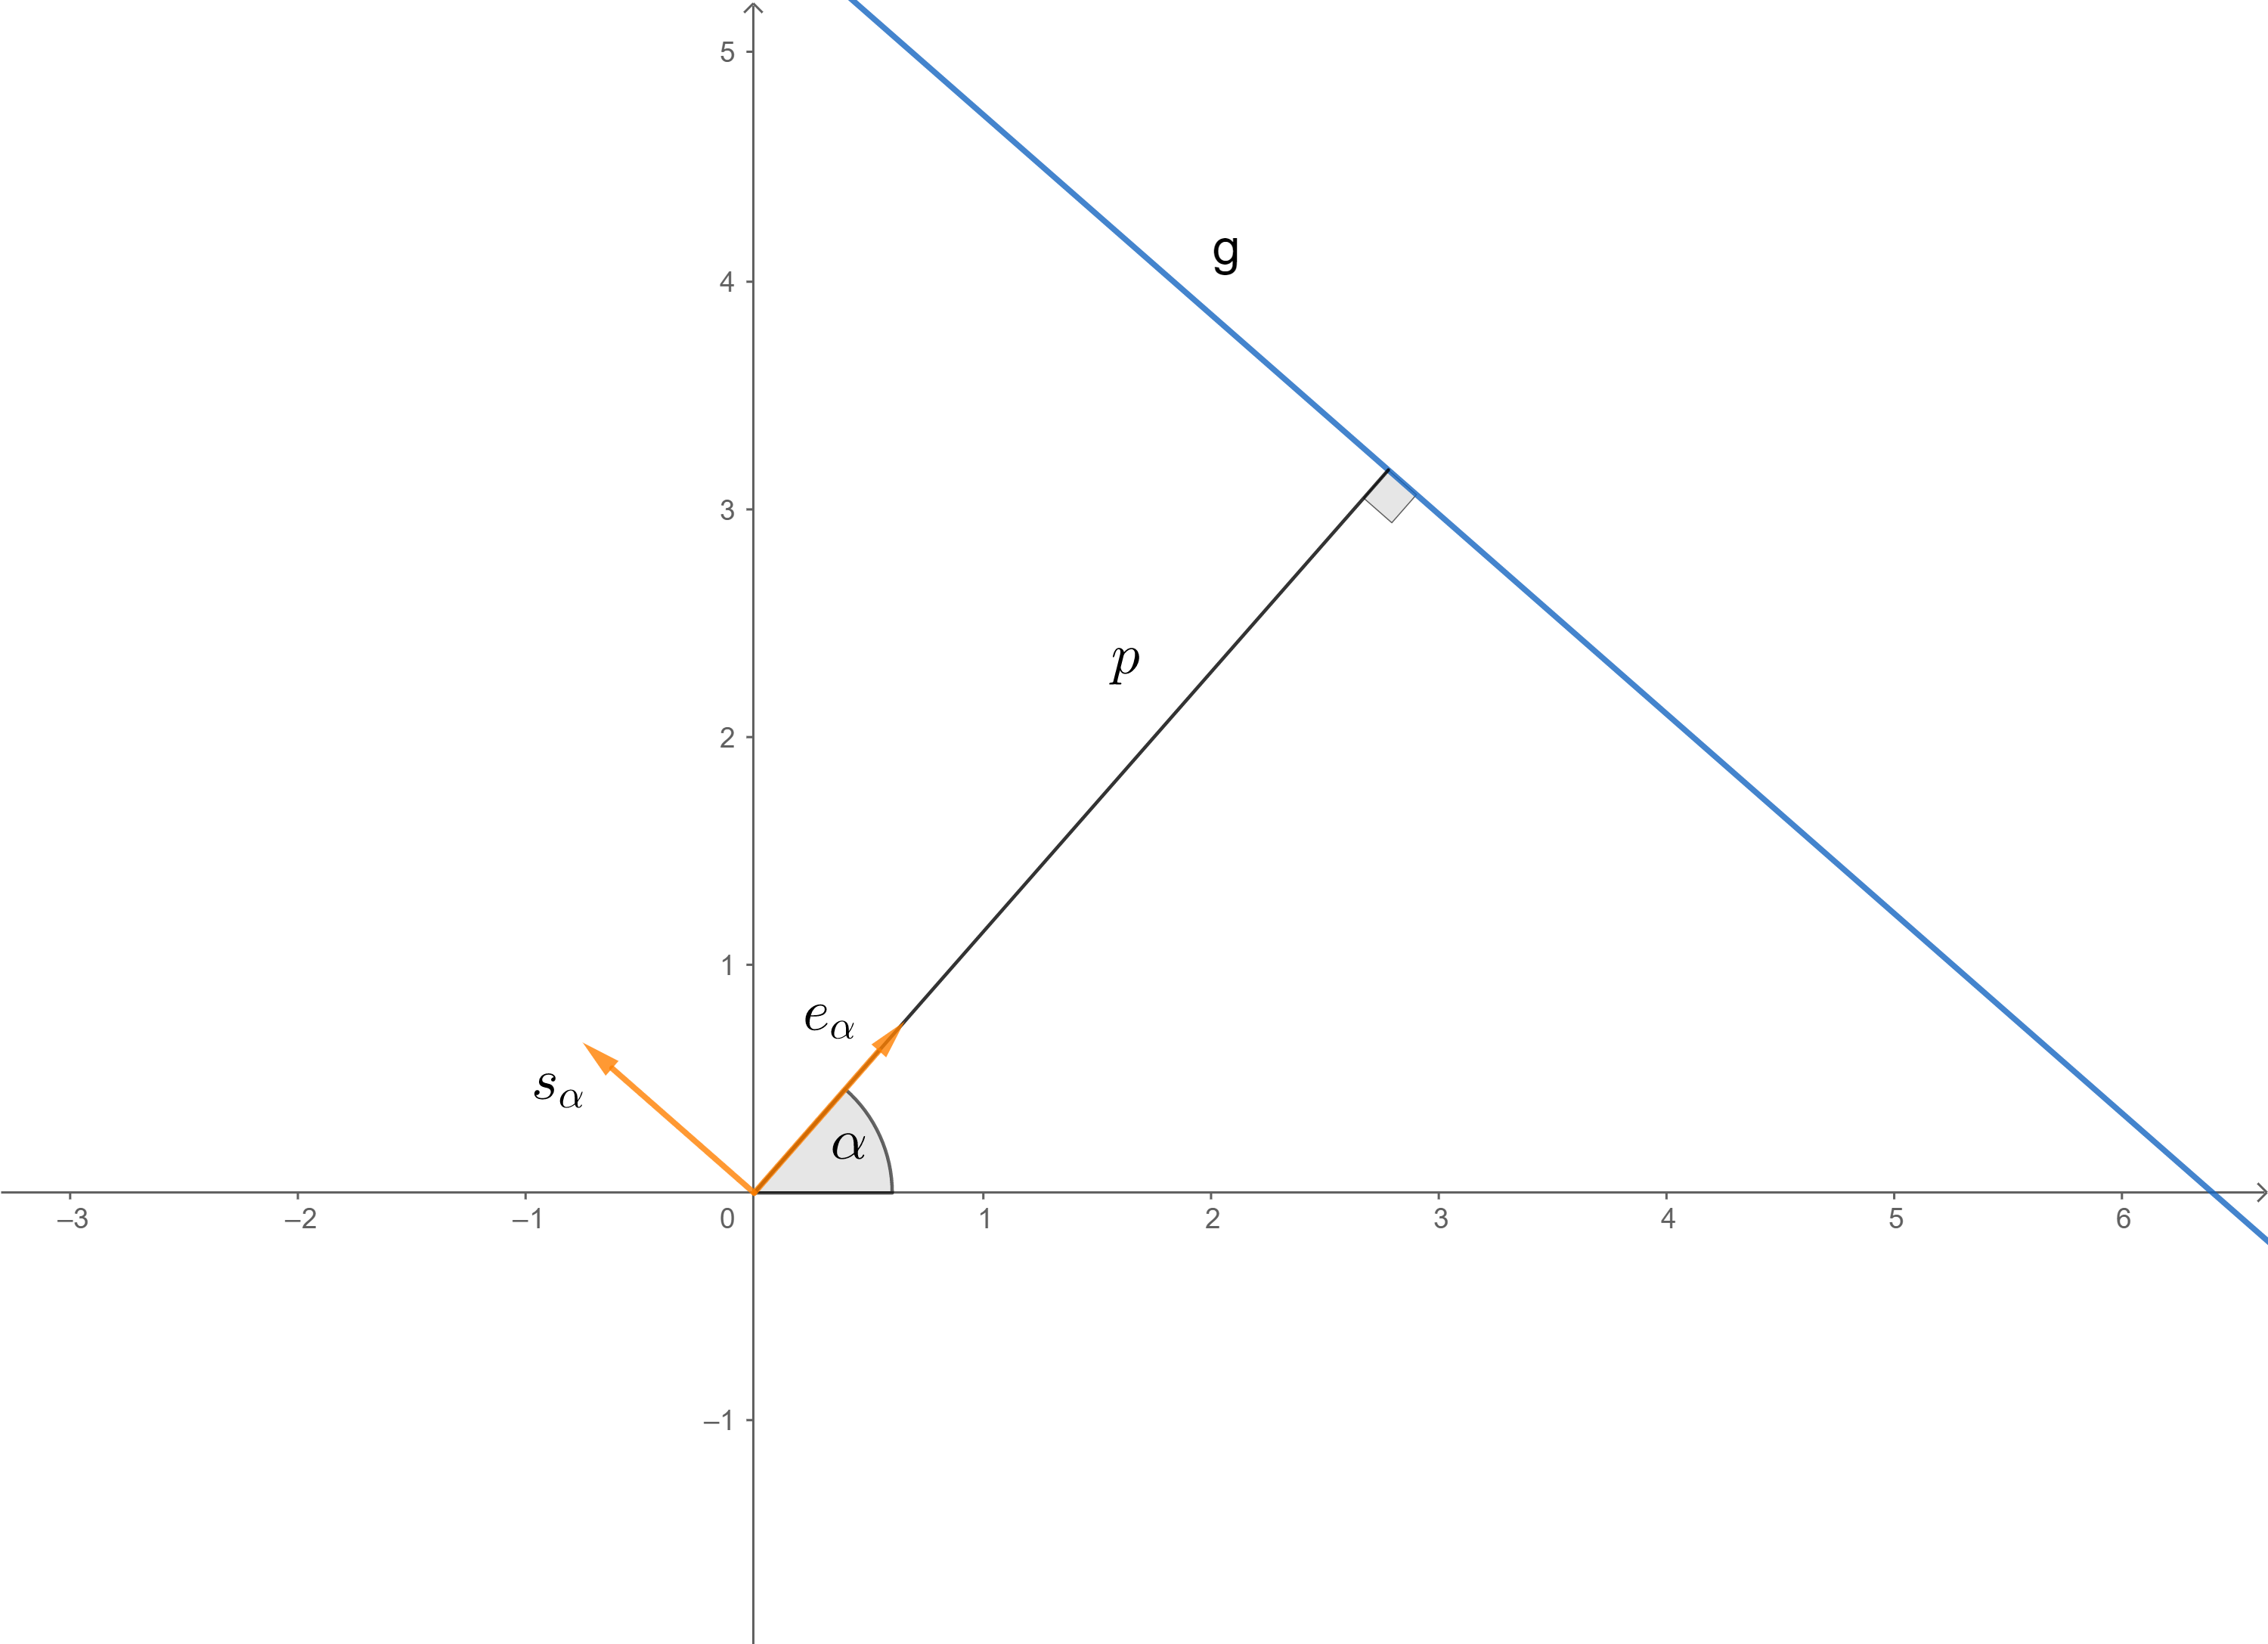
\includegraphics[height=10cm]{images/geogebra-images/line-param.png}
		\caption{Line parameters $\alpha$ and $p$} \label{lineparam}
	\end{figure}
	


\begin{figure}[]
	\centering
	\begin{subfigure}[b]{.49\textwidth}
		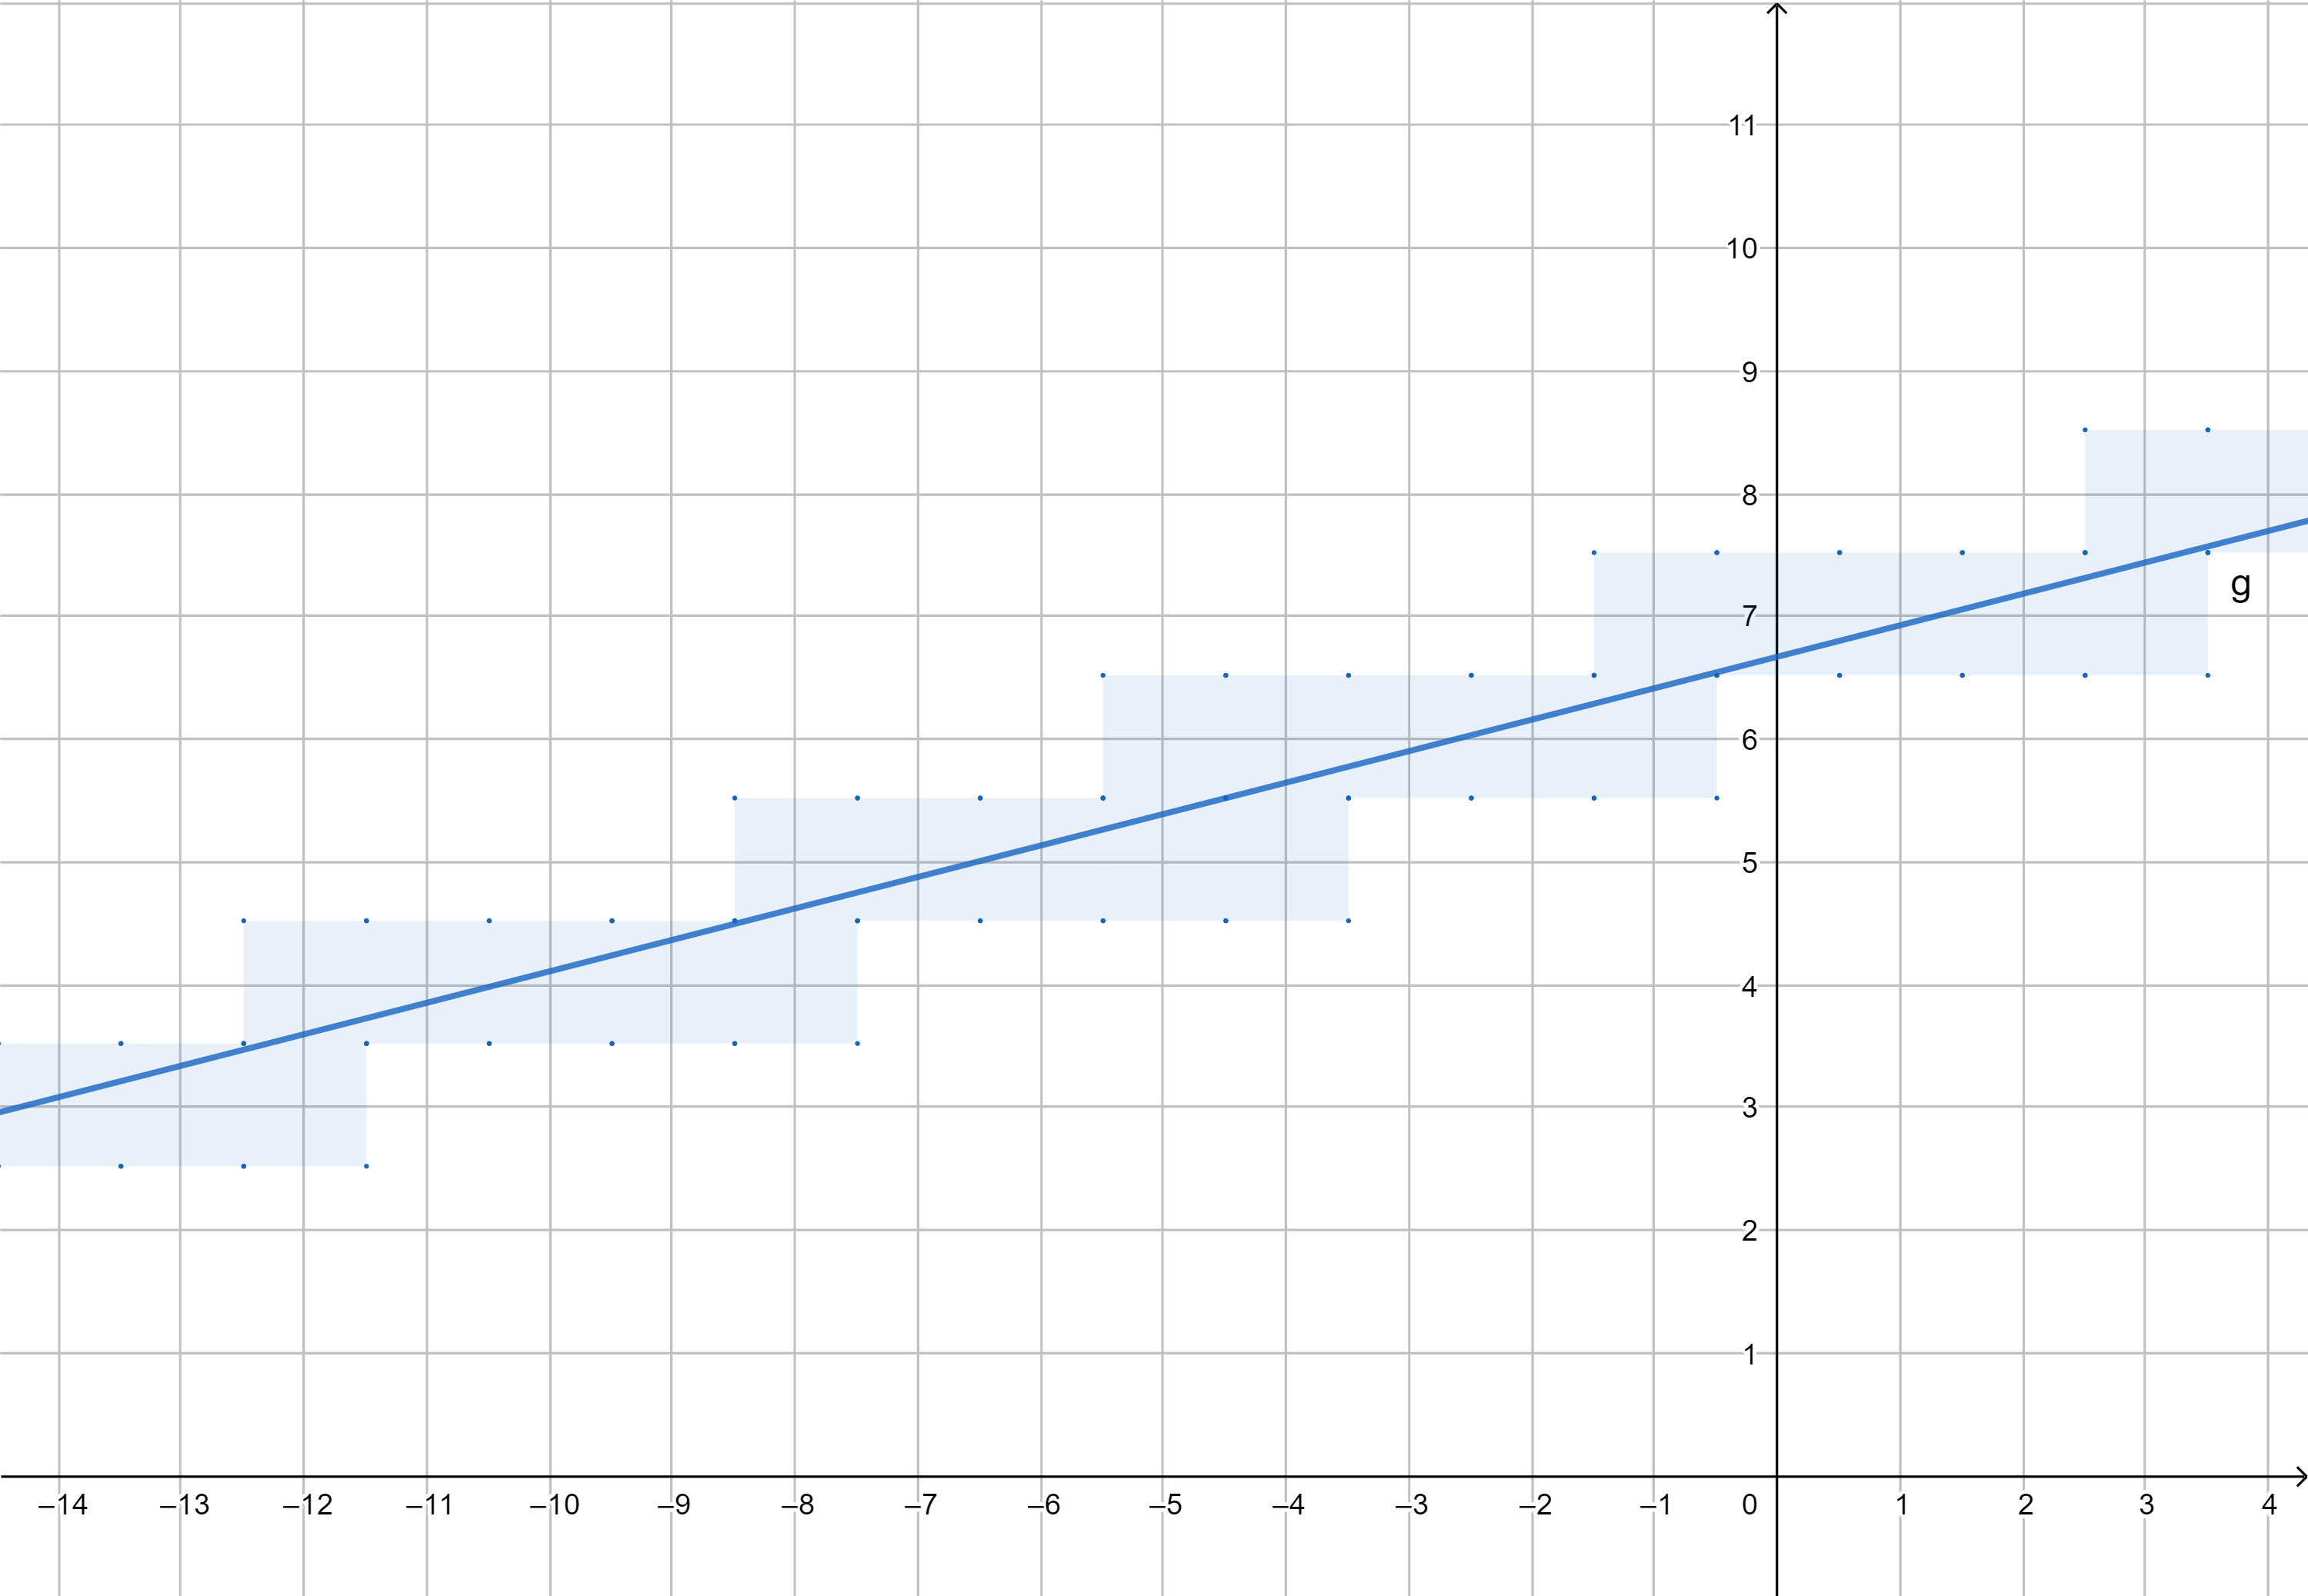
\includegraphics[width=1\linewidth]{images/geogebra-images/line-hit-squares.png}
	\end{subfigure}
	\begin{subfigure}[b]{.49\textwidth}
		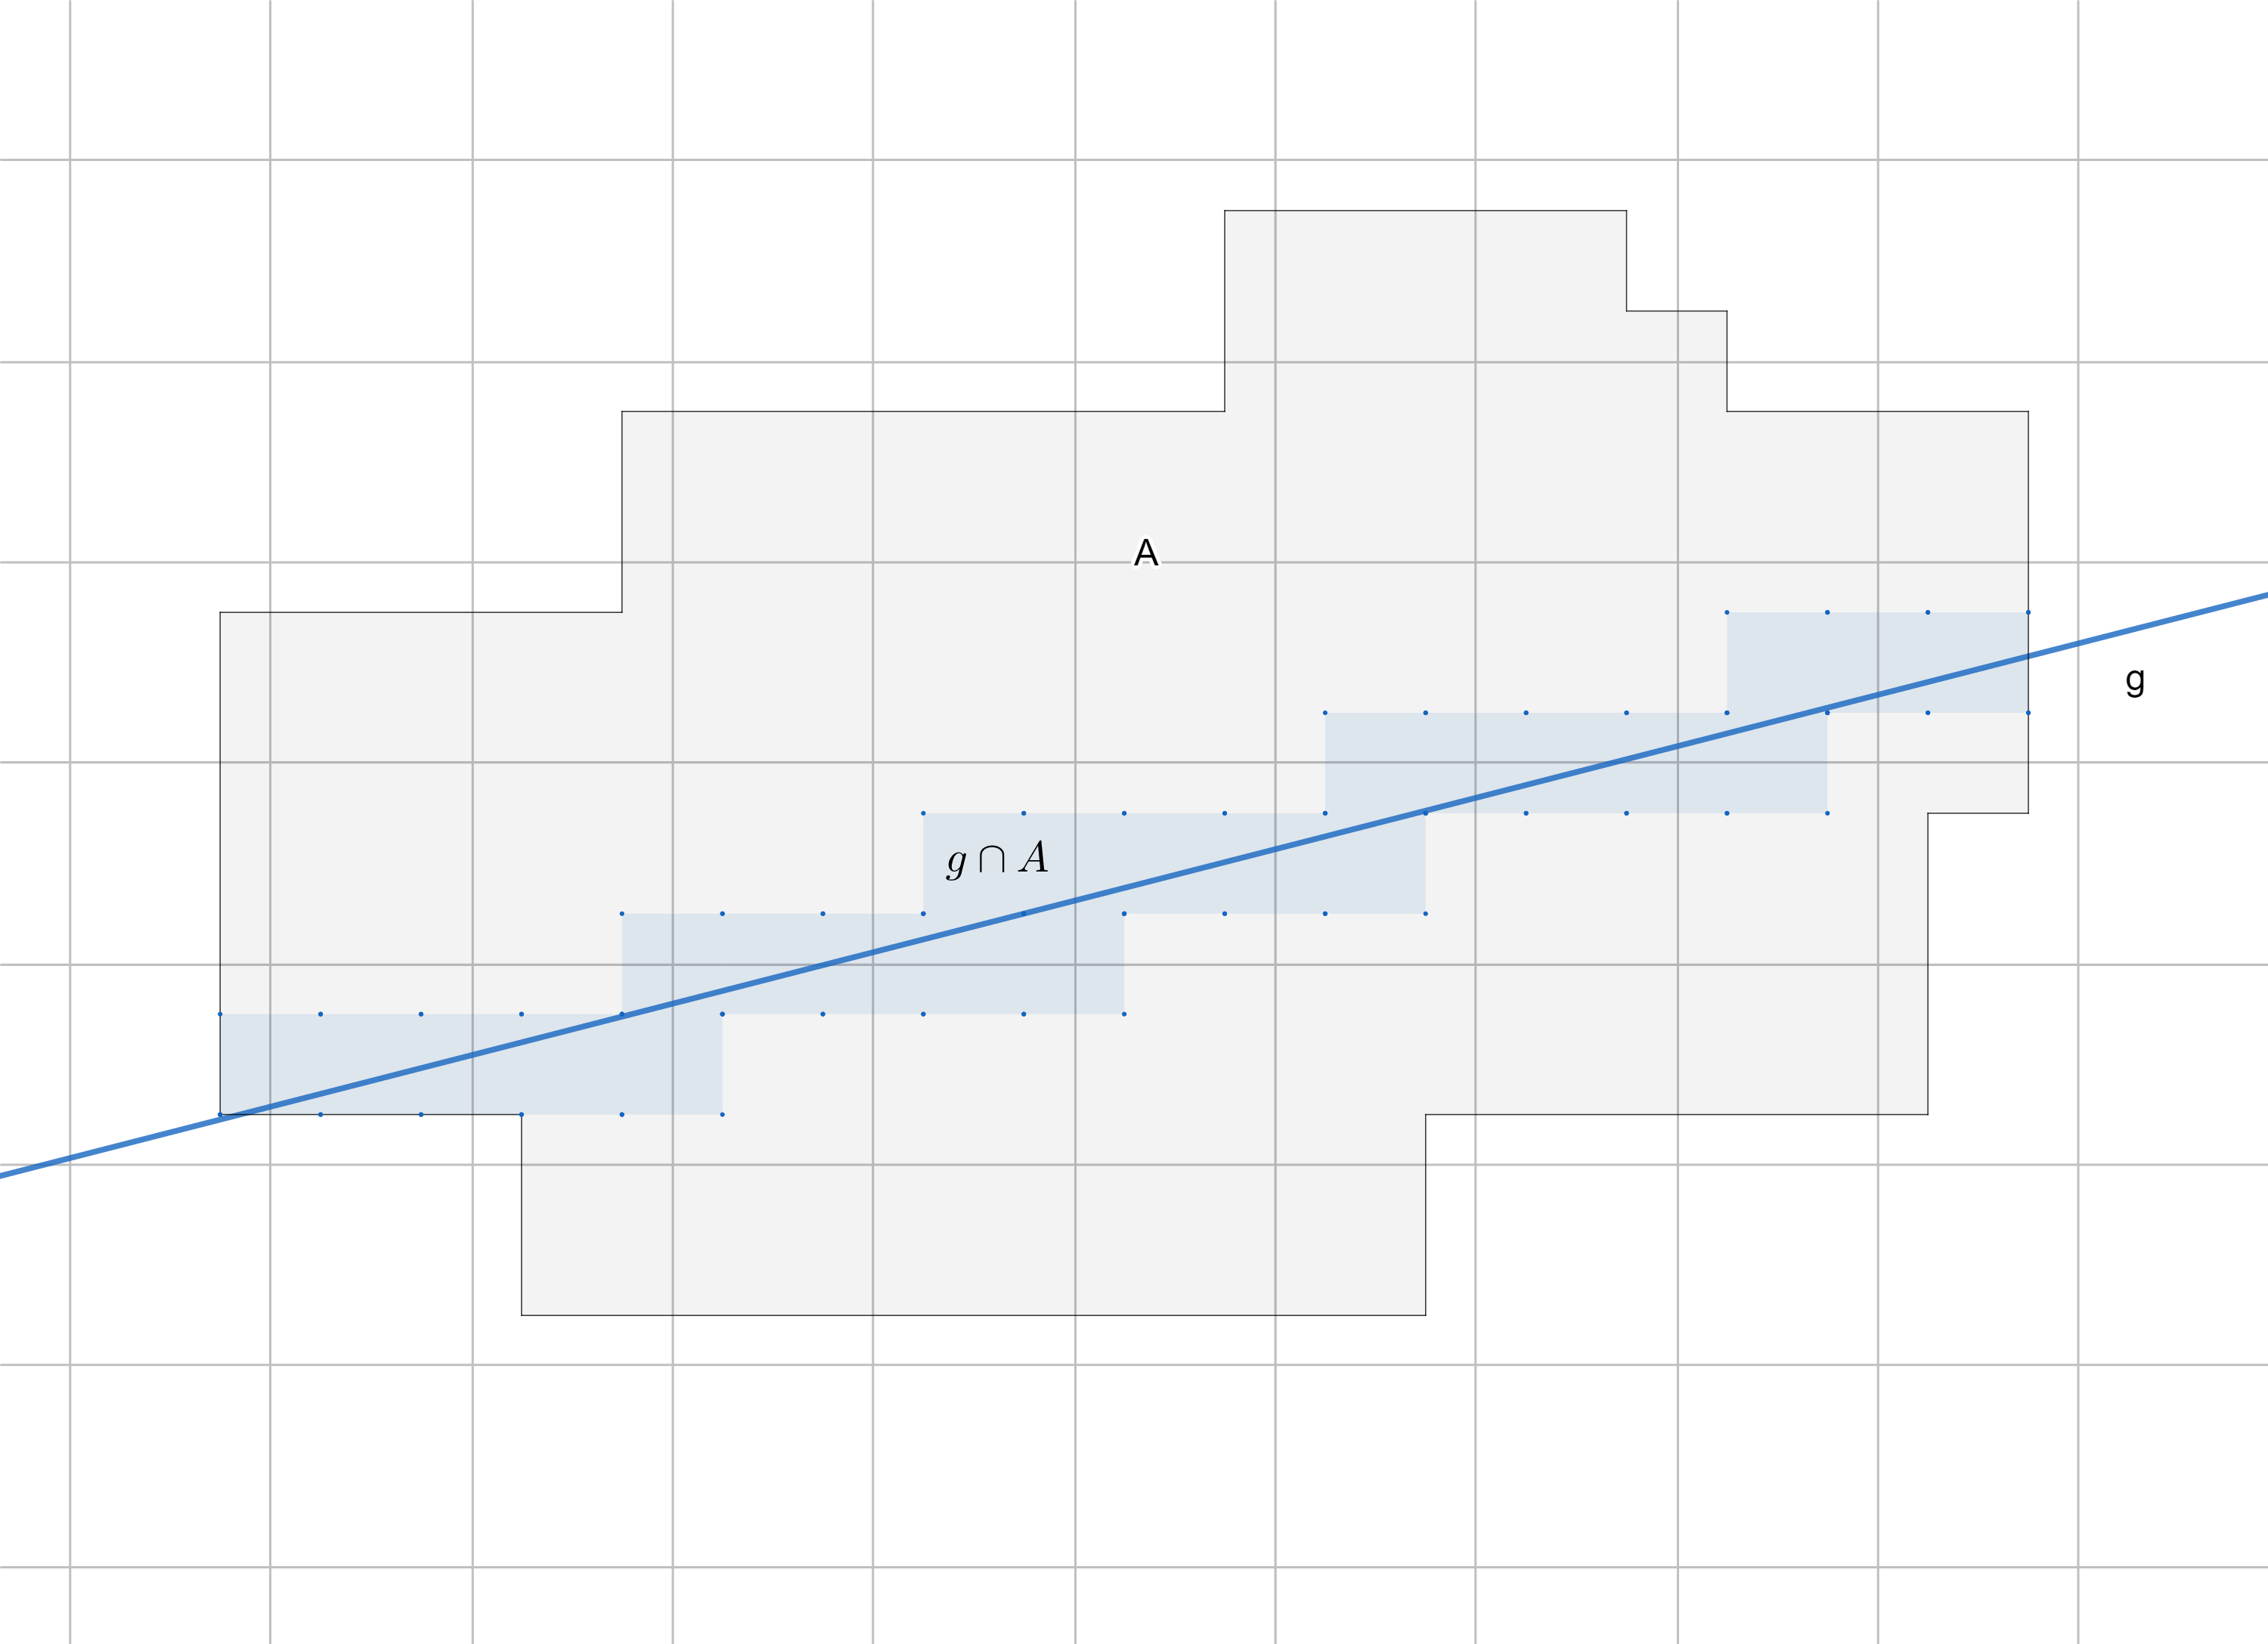
\includegraphics[width=1\linewidth]{images/geogebra-images/line-hit-A.png}
	\end{subfigure}
	\caption{Line hitting squares}
	\label{linesquares}
\end{figure}

\begin{definition} \label{ghitA}
	Let $g=g_{\alpha,p}\in \G$ and $A\in \mP_f$. We define
	\begin{align*}
		g^A := \{ p\in A\ |\ g \cap sq(p)\neq \emptyset\}
	\end{align*}
	which is the subset of all points in $A$ which are hit by $g$ (see $\autoref{linesquares}$). For the following we suppose $g^A \neq \emptyset$. We will define a total ordered relation $\triangleleft$ on $g^A$ which shall be defined equivalently for all $g\in \G$ and $A\in\mP_f$ with $g^A \neq\emptyset$. We choose two points $x,y\in g^A$ and split the definition of the relation $\triangleleft$ into four cases, depending on whether the line $g$ goes from left-bottom to right-top, left-top to right-bottom, parallel to the $x$-axis or parallel to the $y$-axis. Denote the real part of $x$ with $\re(x)$ and the imaginary part with $\im(x)$. \\
	\\
	$\mathit{Case}\ 1:\quad g\ \text{ is parallel to the x-axis}\quad (\Leftrightarrow\quad \alpha = \frac{\pi}{2})$
	\begin{align*}
	x \triangleleft y \quad :\Leftrightarrow \quad \re(x) < \re(y)
	\end{align*}\\
	$\mathit{Case}\ 2:\quad g\ \text{ is parallel to the y-axis}\quad (\Leftrightarrow\quad \alpha = 0)$
	\begin{align*}
	x \triangleleft y \quad :\Leftrightarrow \quad \im(x) < \im(y)
	\end{align*}\\
	$\mathit{Case}\ 3:\quad g\ \text{ is going from left-bottom to right-top}\quad (\Leftrightarrow\quad \alpha\in (\frac{\pi}{2},\pi))$
	\begin{align*}
	x \triangleleft y \quad :\Leftrightarrow \quad
		\begin{cases}
			\re(x) < \re(y), & \text{ if } \re(x) \neq \re(y), \\
			\im(x) < \im(y), & \text{ if } \re(x) = \re(y).
		\end{cases}
	\end{align*}\\
	$\mathit{Case}\ 4:\quad g\ \text{ is going from left-top to right-bottom}\quad (\Leftrightarrow\quad \alpha\in (0,\frac{\pi}{2}))$
	\begin{align*}
	x \triangleleft y \quad :\Leftrightarrow \quad
	\begin{cases}
	\re(x) < \re(y), & \text{ if } \re(x) \neq \re(y), \\
	\im(x) > \im(y), & \text{ if } \re(x) = \re(y).
	\end{cases}
	\end{align*}\\
	It is easy to calculate that this defines a well-defined relation on $g^A$. In the following we will prove that this relation is totally ordered. 
\end{definition}

\begin{lemma}
	For a line $g=g_{\alpha,p}\in\G$ and $A\in \mP_f$ with $g^A\neq \emptyset$ the relation $\triangleleft$ on $g^A$ is totally ordered. 
\end{lemma}

\begin{proof}
	We will only prove the case where $g$ is going from left-bottom to right-top, which is $\mathit{Case}\ 3$ of the definition. In this case we have $\alpha\in (\frac{\pi}{2},\pi)$. Note, that the proof for $\mathit{Case\ }4$ will work very similar and in the case of $g$ being parallel to one of the axes ($\mathit{Case\ }1$ or $2$), all properties for a totally ordered relation follow directly from the totally ordered relation $<$ on $\mathbb{R}$. So let $\alpha\in (\frac{\pi}{2},\pi)$. \\
	\\
	$\mathit{Antisymmetry:}$ For antisymmetry let $x \triangleleft y$ and $y \triangleleft x$. Suppose $\re(x)\neq \re(y)$, then $\re(x) < \re(y)$ and $\re(y) < \re(x)$, a contradiction because of the total order $<$ in $\mathbb{R}$. So $\re(x) = \re(y)$. But then we have $\im(x) < \im(y)$ and $\im(y) < \im(x)$ and therefore also $\im(x) = \im(y)$, hence $x=y$. \\
	\\
	$\mathit{Transitivity:}$ For transitivity let $x \triangleleft y$ and $y \triangleleft z$. We find four cases. In case $\re(x) \neq \re(y)$ and $\re(y) \neq \re(z)$ we get $\re(x) < \re(z)$ by transitivity of $<$, hence $x \triangleleft z$. In case $\re(x)\neq \re(y)$ and $\re(y) = \re(z)$ we get $\re(x) < \re(y) = \re(z)$, therefore $x \triangleleft z$. In case $\re(x) = \re(y)$ and $\re(y) \neq \re(z)$ we get $\re(x) = \re(y) < \re(z)$, similar as the last case. In the last case $\re(x) = \re(y) = \re(z)$ we get $\im(x) < \im(y)$ and $\im(y) < \im(z)$ and again by transitivity of $<$ we get $\im(x) < \im(z)$, hence $x \triangleleft z$ again. \\
	\\
	$\mathit{Connexity:}$ Connexity is given since for any two points $x,y\in g^A$ we have either $\re(x) \neq \re(y)$ or $\re(x) = \re(y)$ and therefore either $x\triangleleft y$ or $y\triangleleft x$.
\end{proof}

\begin{remark}
	The relation $\triangleleft$ on $g^A$ basically orders the hitting points of $g$ with $A$ from left to right (or bottom to top in case of a line parallel to the $y$-axis). This order allows us to identify the outermost hitting points which are the minimum and maximum of $g^A$ with respect to $\triangleleft$. To clarify, we define $\min_\triangleleft (g^A) := x_0$ if and only if $x_0 \triangleleft x$ for all $x\in g^A,x\neq x_0$, analogously $\max_\triangleleft(g^A)$. This means when moving on $g$ facing $A$ coming from infinity this order allows to know where the line $g$ hits $A$ first and where it hits $A$ last. What we want to do next is to choose a line randomly and fair out of all lines which hit the current cluster. This is isn't obvious and we will have to develop and argue a most fair underlying distribution on lines in the next section where we will touch basic aspects of Integral Geometry. 
\end{remark}


\subsection{Excursion: Integral geometry}

In the next section we want to define an incremental aggregation for which distribution we need some concepts and results from integral geometry. We will want to fairly choose a random line out of all lines which intersect the current cluster. It is not obvious how to choose a line in a fair way since most of the time the cluster will be strongly non symmetric. We will introduce a possible solution for this problem through the parametrisation of lines as defined in \ref{linedef} for the $2$-dimensional case which goes hand in hand with a more general result of integral geometry which we will touch first.

\subsubsection{General results}

Let $d\in\N$ and $q\in \{0,\dots,d\}$. In the general context we are in $\R^d$ and consider $q$-dimensional affine subspaces, short $q$-flats. The set of $q$-flats in $\R^d$ we denote with $A(d,q)$. Later we will be interested in choosing random lines in the plane (i.e. $1$-flats in $\R^2$). In order to get a probability measure on some set of $q$-flats, we first need a measure and a $\sigma$-algebra on $A(d,q)$ in total. Recall that we denote the set of convex and compact subsets of $\R^d$ with $\K^d$. Also recall that with $G_d$ we denote the set of all Euclidean motions (as defined in \ref{symbols}).

\begin{definition}
	For $B\in \mathcal{B}^d$ define 
	\begin{flalign*}
		[B]_{d,q} := \{F\in A(d,q)\ |\ F\cap B \neq\emptyset\}.
	\end{flalign*}
	If the context is clear, we will only write $[B]$ instead of $[B]_{d,q}$. 
\end{definition}

\begin{definition}\label{generalsigma}
	The $\sigma$-algebra $\mathcal{A}(d,q)$ on $A(d,q)$ is defined by
	\begin{flalign*}
		\mathcal{A}(d,q) := \sigma(\{ [K]\ |\ K\in \K^d\}).
	\end{flalign*} 
\end{definition}

\begin{remark} \label{uniqmeas}
	It can be shown that on $A(d,q)$ there exists an unique $G_d$-invariant Radon measure $\mu_q$ such that 
	\begin{flalign}
		\mu_q([B_d(0,1)]) = \kappa_{d-q}, 
	\end{flalign}
	where $\kappa_n := \lambda_n(B_n(0,1))$ is the $n$-dimensional Lebesque meausure of the $n$-dimensional unit ball for $n\in \N$ and $\kappa_0:=1$. We won't argue that further here. For more information see at \cite{stoch1}. 
\end{remark}

\subsubsection{Construction in the plane: Isotropic lines}

For our special case we choose $d=2$ and $q=1$, thus lines in the plane. We want to show in the following that the way we defined a $\sigma$-algebra on $\G$ in Definition \ref{linedef} is equivalent to the general Definition \ref{generalsigma}. To do that it is convenient to use a special generator set for the Borel-$\sigma$-algebra $\mathcal{B}_\Phi$. 

\begin{lemma} \label{generators}
	Define 
	\begin{flalign*}
		\mathcal{R}_+ := \{[\alpha,\beta]\times (0,b]\ |\ 0\leq \alpha<\beta<\pi, b \geq 0\}, 
	\end{flalign*}
	\begin{flalign*}
		\mathcal{R}_- := \{[\alpha,\beta]\times [b,0)\ |\ 0\leq \alpha<\beta<\pi, b\leq 0\},
	\end{flalign*}
	\begin{flalign*}
		\mathcal{R}_0 := \{[\alpha,\beta]\times \{0\}\ |\ 0\leq \alpha<\beta<\pi\},
	\end{flalign*}
	and
	\begin{flalign*}
		\mathcal{R} := \mathcal{R}_+ \cup \mathcal{R}_- \cup \mathcal{R}_0.
	\end{flalign*}
	Then $\sigma(\mathcal{R}) = \mathcal{B}_\Phi$.
\end{lemma}
\begin{proof}
	We show that $\sigma(\mathcal{R})$ contains all rectangles in $\Phi$ of the form $[\alpha,\beta]\times (a,b]$ with $a,b>0$, $[\alpha,\beta]\times [a,b)$ with $a,b<0$ and $[\alpha,\beta]\times [a,b]$ with $0\in [a,b]$. First let $a,b>0$ and $R=[\alpha,\beta]\times (a,b]$, then 
	\begin{flalign*}
		R = ([\alpha,\beta] \times (0,b]) \setminus ([\alpha,\beta] \times (0,a])
	\end{flalign*}
	and therefore $R\in \sigma(\mathcal{R}_+)\subset\sigma(\mathcal{R})$. Similarly it works if $a,b<0$. If $0\in[a,b]$ then we can write $R = [\alpha,\beta]\times [a,b]$ with three components $R = [\alpha,\beta] \times [a,0) \cup [\alpha,\beta] \times \{0\} \cup [\alpha,\beta] \times (0,b]$ which lie in $\mathcal{R}_-, \mathcal{R}_0$ and $\mathcal{R}_+$ respectively. Therefore $R\in \sigma(\mathcal{R})$ as well. By measure theory the above described rectangles form a generator set of $\mathcal{B}_\Phi$, which completes the proof. 
\end{proof}

\begin{lemma}
	We have $\mathcal{A}(2,1) = \GG$. 
\end{lemma}
\begin{proof}
	We will consider generators of these $\sigma$-algebras. By Lemma $\autoref{generators}$ we know that $\sigma(\mathcal{R}) = \mathcal{B}_\Phi$ and since $\chi$ is a bijection, we have $\chi(\sigma (\mathcal{R})) = \sigma (\chi(\mathcal{R}))$ and finally $\GG = \sigma(\chi(\mathcal{R}))$. For $\tilde A := \{[K]\ |\ K\in \K^2\}$ we have by definition $\mathcal{A}(2,1) = \sigma(\tilde A)$. \\
	\\ \indent $\subset$: Let $K\in\K^2$. We will show that $\chi^{-1}([K])$ is a closed set in $\Phi$. If that is the case we have $\chi^{-1}([K])\in\mathcal{B}_\Phi$, therefore $[K] \in\chi(\mathcal{B}_\Phi) = \GG$ and finally $\mathcal{A}(2,1) = \sigma(\tilde A)\subset\GG$. To show that $\chi^{-1}([K])$ is closed let $(\alpha_0,p_0)\in \Phi\setminus \chi^{-1}([K])$. Then $\chi(\alpha_0,p_0) \notin [K]$ and therefore $\chi(\alpha_0,p_0) \cap K= \emptyset$. Since $K$ is closed we can find small values $\tilde\alpha,\tilde p > 0$ such that $\chi(\alpha,p) \cap K = \emptyset$ for all $(\alpha,p)\in [\alpha_0, \alpha_0 + \tilde\alpha] \times [p_0, p_0 + \tilde p] =: R$. Hence we have $ R\subset \Phi \setminus \chi^{-1}([K])$, so $\Phi \setminus \chi^{-1}([K])$ is open. Hence $\chi^{-1}([K])$ is closed. \\
	\\ \indent $\supset$: For this inclusion we will show that $\chi(R)\in\mathcal{A}(2,1)$ for all $R\in\mathcal{R}$. First let $R = [\alpha,\beta]\times(0,b]\in\mathcal{R}_+$ for some $b>0$. Define 
	\begin{flalign*}
		S:= \{pe_\gamma \in \C\ |\ (\gamma,p)\in R\}
	\end{flalign*}
	Furthermore for $n\in \N$ define 
	\begin{flalign*}
		A_n := \{tns_\beta\ |\ t\in [0,1]\} \text{ and } B_n := \{-tns_\alpha\ |\ t\in [0,1]\},
	\end{flalign*}
	the segments from $0$ to $ns_\beta$ and $0$ to $-ns_\alpha$ ($\autoref{circleS}$). We will show now that 
	\begin{flalign*}
		\chi(R) = [\bar S] \setminus (\bigcup_{n\in\N} [A_n] \cup \bigcup_{n\in\N} [B_n]) =: \tilde S,  
	\end{flalign*}
	
	\begin{figure}
		\centering
		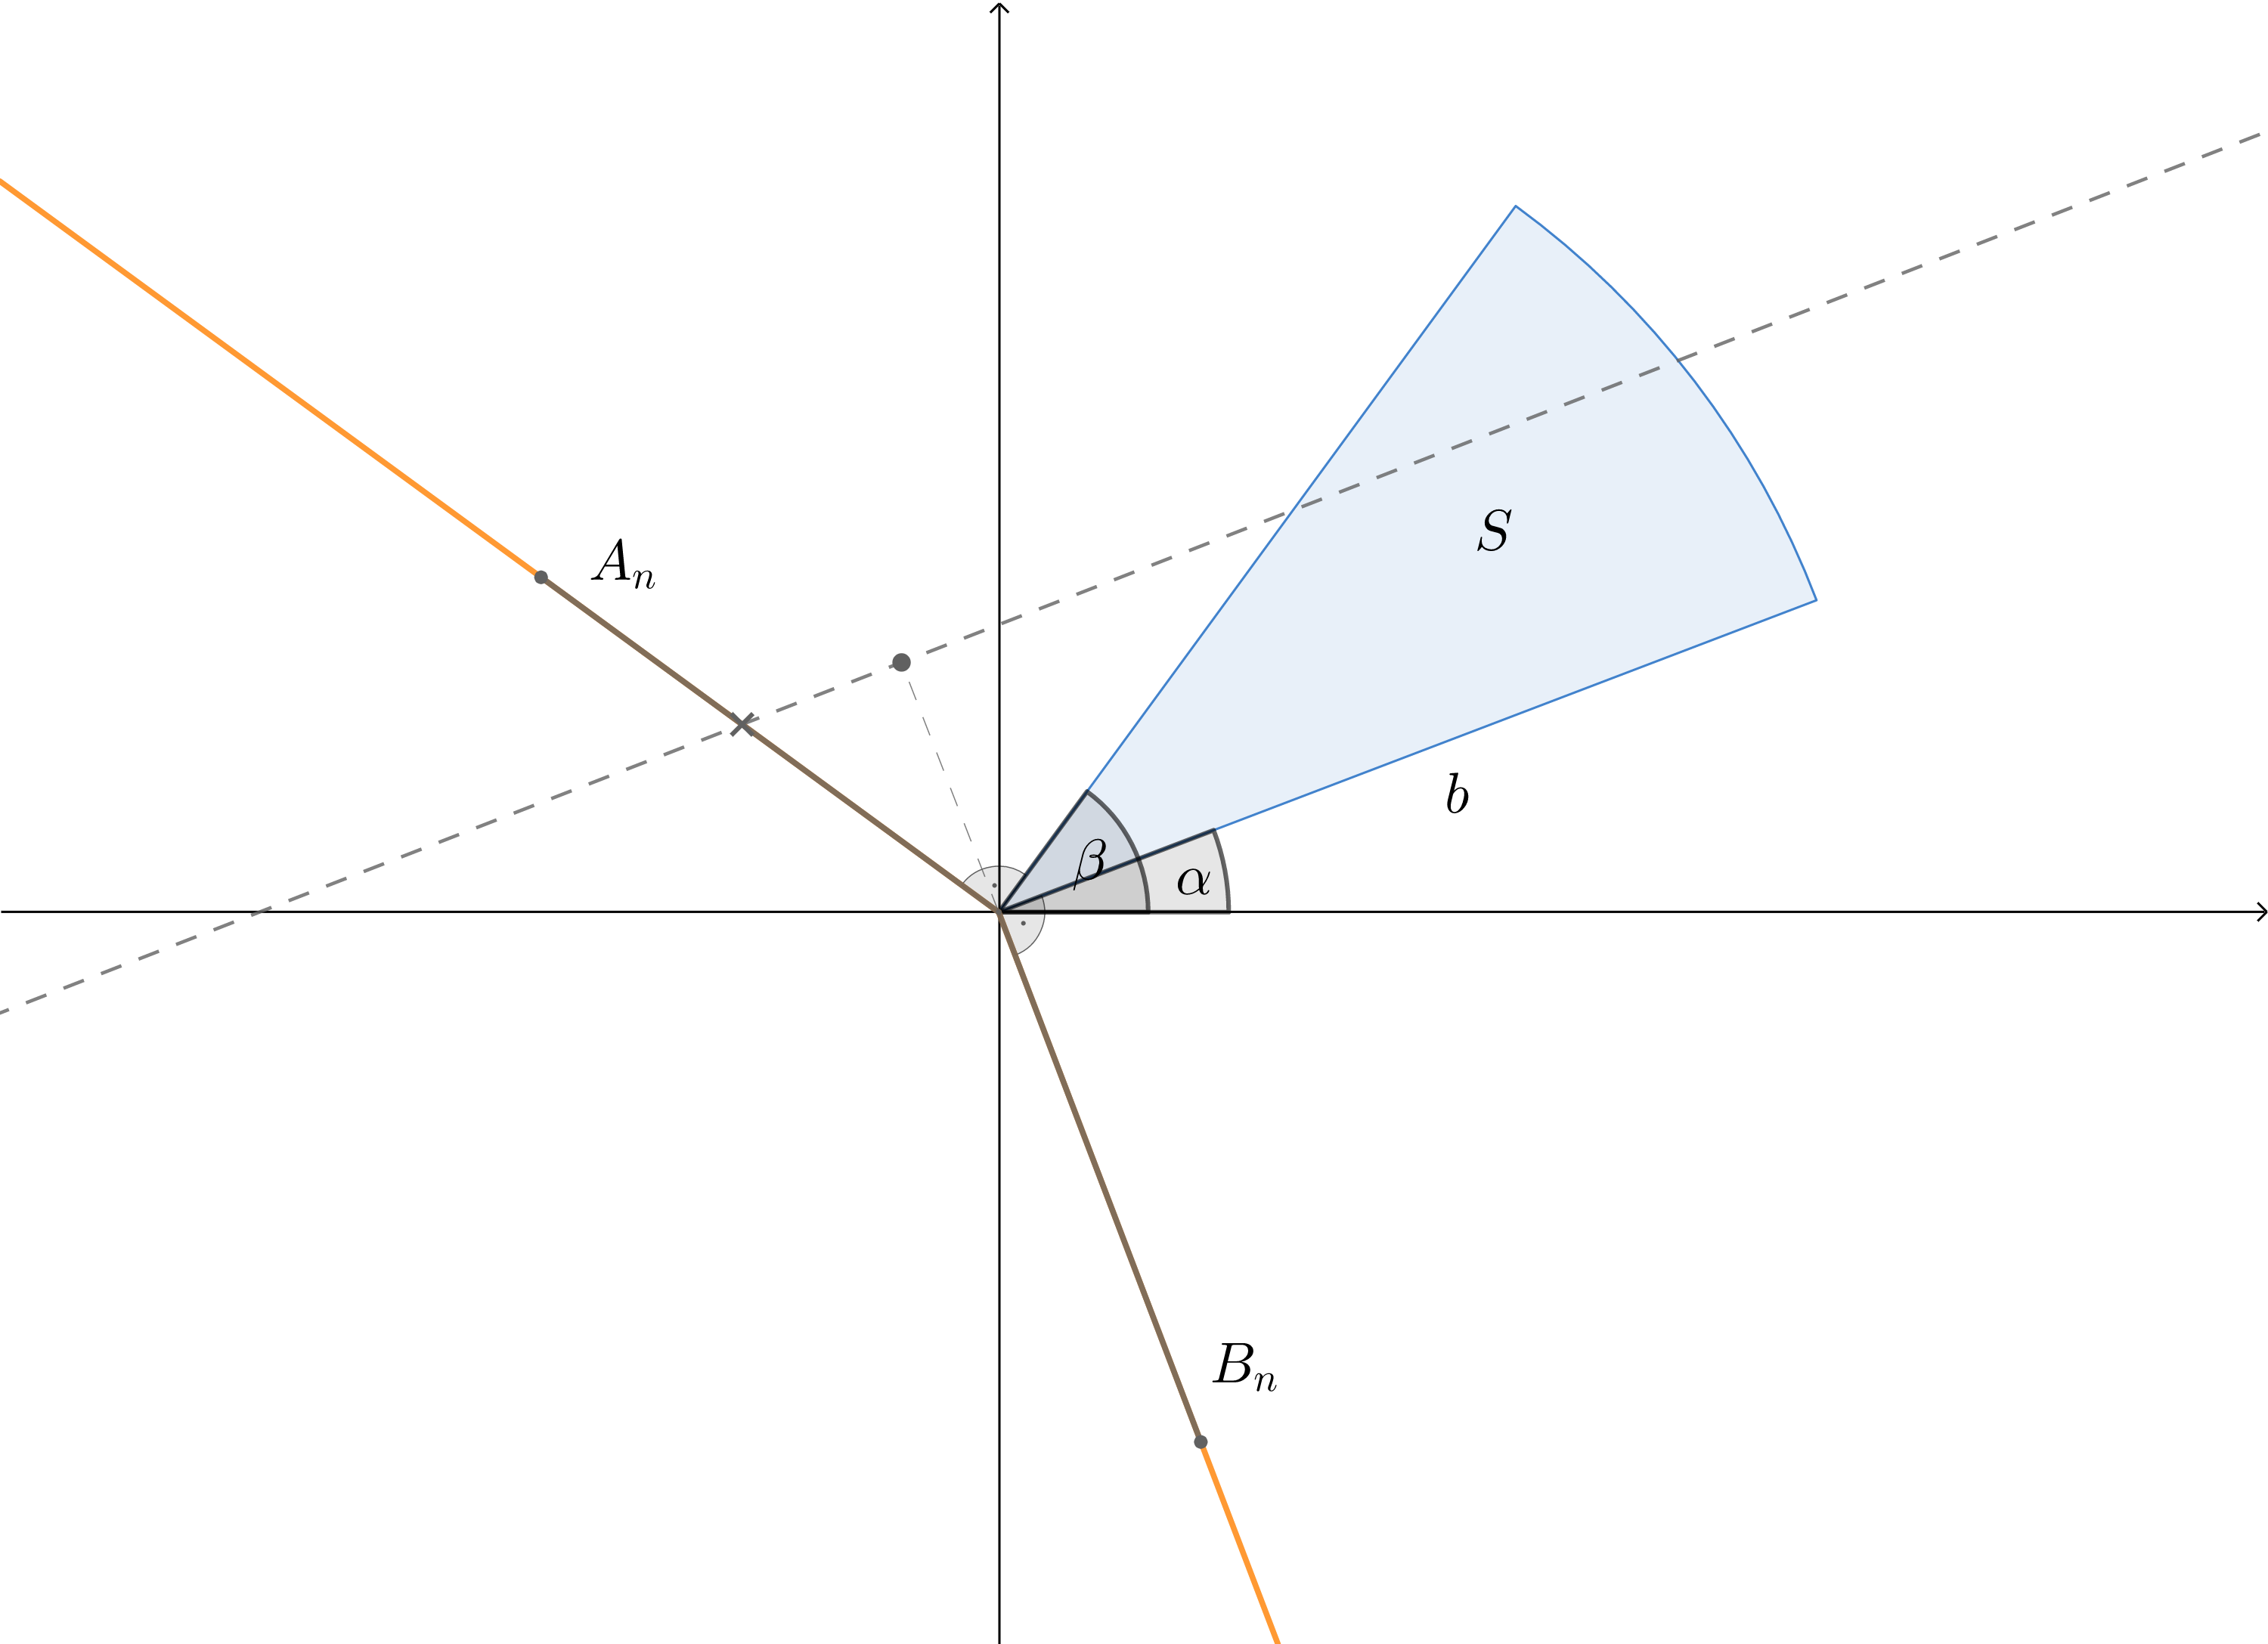
\includegraphics[height=10cm]{images/geogebra-images/circle-part-S.png}
		\caption{$S$ and the sets $A_n$ and $B_n$} \label{circleS}
	\end{figure}
	
	where $\bar S$ is the closure of $S$ as a set in $\C$ (note that $\bar S = S\ \cup\ \{0\}$). Let $(\gamma,p)\in R$. Then $pe_\gamma\in \chi(\gamma,p)\cap S$ and therefore $\chi(\gamma,p)\in [\bar S]$. Assume that there exits an $n\in\N$ such that $\chi(\gamma,p)\cap A_n \neq \emptyset$. Then $\beta + \frac{\pi}{2} - \gamma < \frac{\pi}{2}$, hence $\beta < \gamma$, a contradiction. Similarly argument for any $B_n$, so we finally have $\chi(\gamma,p) \notin [A_n]$ and $\chi(\gamma,p) \notin [B_n]$ for any $n\in \N$. Hence $\chi(\gamma,p)\in\tilde S$ and therefore $\chi(R)\subset \tilde S$. \\
	\\
	Now let $(\gamma,p)\in\Phi$ such that $\chi(\gamma,p)\in \tilde S$. Assume that $\gamma\notin[\alpha,\beta]$ then with a similar argument as in the first inclusion it is easy to see that there must be an $n\in\N$ such that $\chi(\gamma,p)\cap A_n\neq \emptyset$ or $\chi(\gamma,p)\cap B_n\neq \emptyset$, a contradiction. Therefore $\gamma\in[\alpha,\beta]$. Now assume $p\notin (0,b]$. If $p>b$ then $\chi(\gamma,b)\cap B_b = \emptyset$ and since $\bar S\subset B_b$ it is $\chi(\gamma,p)\notin [\bar S]$, a contradiction. If $p<0$ then, since the angle between the segments $A_n$ and $B_n$ opposite of $S$ is strictly smaller than $\pi$, $\chi(\gamma,p)$ must intersect with $A_n$ or $B_n$ for some $n\in\N$, again a contradiction. Note that $p\neq 0$ since $[\{0\}] \subset [A_1]$. Thus we have $p\in(0,b]$. Therefore we have $(\gamma,p)\in R$ and finally $\tilde S\subset \chi(R)$. \\
	\\
	It is left to show that $\tilde S\in \mathcal{A}(2,1)$. All the segments $A_n$ and $B_n$ are compact and convex for all $n\in\N$, and since $S$ is bounded and convex as a circle segment with angle smaller than $\pi$, $\bar S$ is compact and convex. Finally $\tilde S\in \mathcal{A}(2,1)$. \\
	\\
	In total we get $\mathcal{R}_+\subset \mathcal{A}(2,1)$. $\mathcal{R}_-\subset \mathcal{A}(2,1)$ can be shown analogously. So for the last case let $R = [\alpha,\beta] \times \{0\}\in \mathcal{R}_0$. Define the line segment
	\begin{flalign*}
		T := \{(1-t)s_\alpha + ts_\beta\ |\ t\in [0,1]\}. 
	\end{flalign*}
	Then $[\{0\}] \cap [T] \in \mathcal{A}(2,1)$. We show that $\chi(R) = [\{0\}] \cap [T]$. Let $(\gamma,0)\in R$. Then $\chi(\gamma,0)$ contains $0$ and since $\gamma$ is in between $\alpha$ and $\beta$, $\chi(\gamma,0)$ must intersect with $T$ ($\autoref{T}$). For the other inclusion let $(\gamma,p)\in\Phi$ such that $\chi(\gamma,p)\in [\{0\}] \cap [T]$. Since $0\in \chi(\gamma,p)$ it must be $p=0$ and since it intersects with $T$ its angle must lay in between $\alpha$ and $\beta$. All in all this completes the proof. 
\end{proof}

\begin{figure}
	\centering
	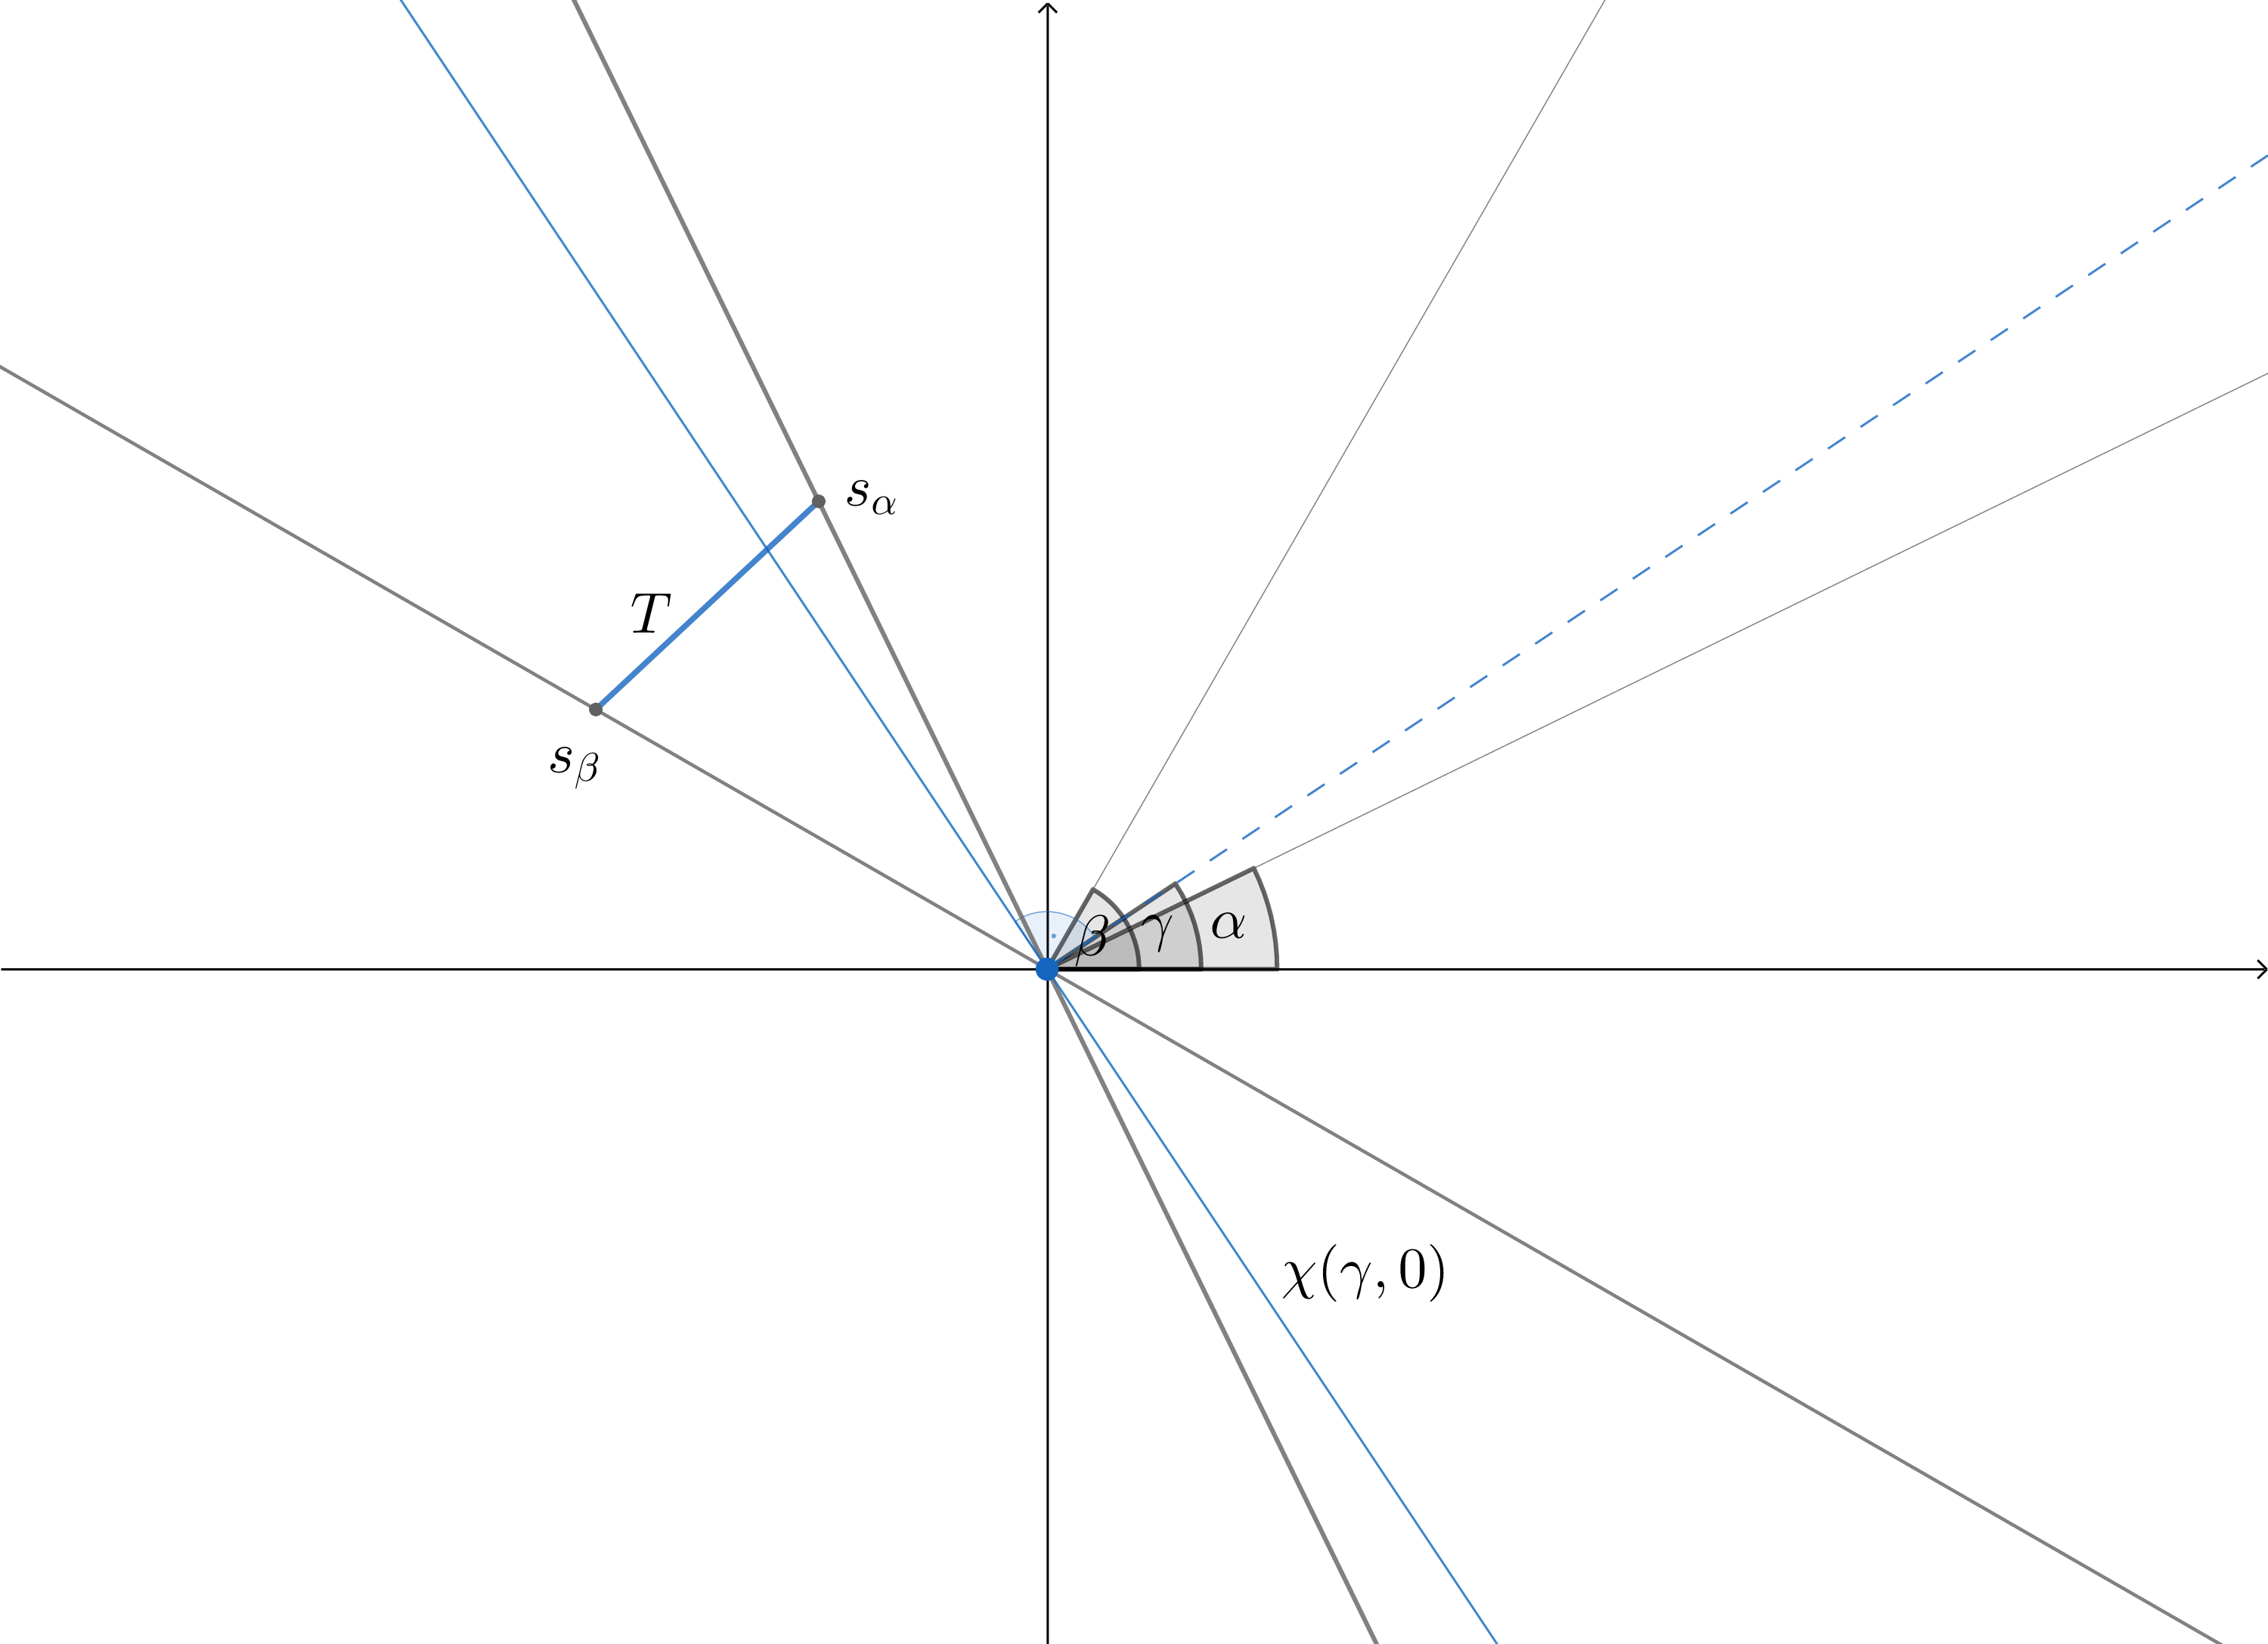
\includegraphics[height=10cm]{images/geogebra-images/T.png}
	\caption{Line in $[\{0\}] \cap [T]$} \label{T}
\end{figure}


\begin{definition}
	A $\mathcal{F}$-$\GG$-measurable function $g:\Omega \to \G$ is called a $\mathit{random\ line}$.  
\end{definition}

\begin{definition}
	We define the measure $\mu := {\lambda_2}_{|\Phi} \circ \chi^{-1}$ on $(\G,\GG)$ where ${\lambda_2}_{|\Phi}$ is the $2$-dimensional Lebesgue measure restricted to $\Phi$. We say a measure $\nu$ on $(\G,\GG)$ is locally finite if for any $K\in \K^2$ we have $\nu([K])<\infty$. 
\end{definition}

\begin{lemma} \label{invariant}
	$\mu$ is locally finite and $G_2$-invariant. 
\end{lemma}
\begin{proof}
	Let $K\in \K^2$ and since $K$ is compact choose $r> 0$ such that $K\subset B_r$. Then we have $[K]\subset [B_r]$ and
	\begin{flalign*}
		\mu([K]) \leq \mu([B_r]) = {\lambda_2}_{|\Phi} (\chi^{-1}([B_r])) = {\lambda_2}_{|\Phi}([0,\pi)\times [-r,r]) = 2\pi r < \infty, 
	\end{flalign*}
	hence $\mu$ is locally finite. To show that $\mu$ is $G_2$-invariant, that is Euclidean motion invariant, we must show it is translation and rotation invariant. First we clarify what exactly translation and rotation mean for lines. We denote $x\ modulo\ r$ as $(x)_r$. For $b\in\C$ and $\beta\in[0,2\pi)$ we define 
	\begin{flalign} \label{motion}
		T_b:\ &\Phi \to \Phi,\quad (\alpha,p) \mapsto (\alpha,p+\langle e_\alpha, b\rangle)
	\end{flalign}
	and
	\begin{flalign} \label{motion2}
		D_{\beta}:\ &\Phi \to \Phi,\quad (\alpha,p) \mapsto ((\alpha + \beta)_{\pi}, \delta((\alpha + \beta)_{2\pi})p), 
	\end{flalign}
	where 
	\begin{flalign*}
		\delta: [0,2\pi) \to \{-1,1\}, \quad \gamma \to \begin{cases}
			1,\ \gamma\in [0,\pi) \\
			-1,\ \gamma\in [\pi,2\pi)
		\end{cases}.
	\end{flalign*}
	It is easy to see that both functions are well-defined. The parameter transformation $T_b$ defines a translation by $b$ of the corresponding line, and analogously $D_\beta$ a rotation by $\beta$. We prove that quickyl here. Let $(\alpha,p)\in \Phi$, then 
	\begin{flalign*}
		x\in \chi(\alpha,p)+b &\Leftrightarrow x-b\in \chi(\alpha,p) \\ 
		&\Leftrightarrow \langle e_\alpha, x-b\rangle = p \\ 
		&\Leftrightarrow \langle e_\alpha, x\rangle = p + \langle e_\alpha, b\rangle \\
		&\Leftrightarrow x\in \chi(\alpha, p + \langle e_\alpha, b\rangle) \\
		&\Leftrightarrow x\in \chi(T_b(\alpha, p))
	\end{flalign*}
	and therefore $\chi(\alpha,p) + b = \chi(T_b(\alpha, p))$. Hence $T_b(\alpha,p)$ are indeed the parameters of the line translated by $b$. For the rotation we look at two cases. First let $(\alpha+\beta)_{2\pi} \in [0,\pi)$, then $\delta((\alpha+\beta)_{2\pi}) = 1$ and $(\alpha+\beta)_\pi = \alpha+\beta$ and therefore 
	\begin{flalign*}
		D_\beta(\alpha,p) = (\alpha+\beta,p).
	\end{flalign*} 
	For the second case let $(\alpha+\beta)_{2\pi} \in [\pi,2\pi)$, then we have $\delta((\alpha+\beta)_{2\pi}) = -1$ and $(\alpha+\beta)_\pi = \alpha+\beta - \pi$ and therefore
	\begin{flalign*}
		D_\beta(\alpha,p) = (\alpha + \beta - \pi, -p).
	\end{flalign*}
	In the second case we have to carefully understand the parametrisation of $\G$, but finally we can see that $D_\beta(\alpha,p)$ are indeed the parameters of the line rotated by $\beta$. \\
	\\We will further show now, that $\mu$ is invariant with respect to both these functions. Let $A\in \GG$, $b\in \C$ and $\nu_\beta\in SO_2$ for some $\beta\in[0,2\pi)$. We will understand $A+b = \{g+b\in \G\ |\ g\in A\}$ and $\nu_\beta A = \{\nu_\beta g\in \G\ |\ g\in A\}$ pointwise, and $g+b = \{x+b\ |\ x\in g\}$ and $\nu_\beta g=\{\nu_\beta x\ |\ x\in g\}$ pointwise as well. We furthermore define $A_p := \{\alpha\in[0,\pi)\ |\ (\alpha,p)\in \chi^{-1}(A)\}$ and $A_\alpha := \{p\in \R\ |\ (\alpha,p)\in \chi^{-1}(A)\}$ for $(\alpha,p)\in \Phi$. For the translation by $b$ we get 
	\begin{flalign*}
		\mu(A+b) 
		&= \int_\GG \1_{A+b}(g) \mu(dg) \\
		&= \int_\GG \1_A(g-b) \mu(dg) \\
		&= \int_\GG \1_A(g-b) {\lambda_2}_{|\Phi}(\chi^{-1}(dg)) \\
		&= \int_{\chi^{-1}(\GG)} \1_{\chi^{-1}(A)}(\chi^{-1}(g-b)) {\lambda_2}_{|\Phi}(d(\chi^{-1}(g))) \\
		&\overset{(\ref{motion})}{=} \int_\Phi \1_{\chi^{-1}(A)}(\alpha,p-\langle e_\alpha, b\rangle) {\lambda_2}(d(\alpha,p)) \\ 
		&= \int_0^\pi \int_\R \1_{A_\alpha}(p-\langle e_\alpha, b\rangle) {\lambda_1}(dp){\lambda_1}(d\alpha) \\ 
		&= \int_0^\pi \int_\R \1_{A_\alpha +\langle e_\alpha, b\rangle}(p) {\lambda_1}(dp)\lambda_1(d\alpha) \\ 
		&= \int_0^\pi \lambda_1(A_\alpha +\langle e_\alpha, b\rangle) {{\lambda_1}_{|[0,\pi)}}(d\alpha) \\ 
		&\overset{(+)}= \int_0^\pi \lambda_1(A_\alpha) \lambda_1(d\alpha) \\ 
		&= \dots \\
		&= \mu(A),
	\end{flalign*}
	and for a rotation we get
	\begin{flalign*}
		\mu(\nu_\beta A) &= \int_\G \1_{\nu_\beta A}(g) \mu(dg) \\
		&= \int_\G \1_A(\nu_{-\beta} g) {\lambda_2}_{|\Phi}(\chi^{-1}(dg))\\
		&= \int_{\chi^{-1}(\G)} \1_{\chi^{-1}(A)}(\chi^{-1}(\nu_{-\beta} g)) {\lambda_2}_{|\Phi}(d(\chi^{-1}(g)))\\
		&\overset{(\ref{motion2})}= \int_\Phi \1_{\chi^{-1}(A)}((\alpha - \beta)_{\pi}, \delta((\alpha - \beta)_{2\pi})p) {\lambda_2}_{|\Phi}(\alpha,p) \\
		&= \int_\Phi \1_{\chi^{-1}(A)}((\alpha - \beta)_{\pi}, \delta((\alpha - \beta)_{2\pi})p) {\lambda_2}_{|\Phi}(\alpha,p) \\
		&= \int_{0}^{2\pi} \int_\R \1_{\chi^{-1}(A)}((\alpha - \beta)_{\pi}, \delta((\alpha - \beta)_{2\pi})p) {\lambda_1}(dp){{\lambda_1}_{|[0,\pi)}}(d\alpha) \\
		&= \int_{0}^{2\pi} \int_\R \1_{A_{(\alpha - \beta)_{\pi}}}(\delta((\alpha - \beta)_{2\pi})p) {\lambda_1}(dp){{\lambda_1}_{|[0,\pi)}}(d\alpha) \\
		&\overset{(+)}= \int_{0}^{2\pi} \int_\R \1_{A_{(\alpha - \beta)_{\pi}}}(p) {\lambda_1}(dp){{\lambda_1}_{|[0,\pi)}}(d\alpha) \\
		&= \int_\R \int_{0}^{2\pi} \1_{\chi^{-1}(A)}((\alpha - \beta)_{\pi}, p) {{\lambda_1}_{|[0,\pi)}}(d\alpha){\lambda_1}(dp) \\
		&= \int_\R \int_{0}^{2\pi} \1_{A_p}((\alpha - \beta)_{\pi}) {{\lambda_1}_{|[0,\pi)}}(d\alpha){\lambda_1}(dp) \\
		&\overset{(+)}= \int_\R \int_{0}^{2\pi} \1_{A_p}(\alpha) {{\lambda_1}_{|[0,\pi)}}(d\alpha){\lambda_1}(dp) \\
		&= \int_\R \int_{0}^{2\pi} \1_{\chi^{-1}(A)}(\alpha,p) {{\lambda_1}_{|[0,\pi)}}(d\alpha){\lambda_1}(dp) \\
		&= \dots \\
		&= \mu(A).
	\end{flalign*}
	where in $(+)$ we used the translation and rotation invariance of the Lebesgue measure. This completes the proof.
\end{proof}

\begin{example} \label{exp1}
	Choose $K:=B_r\in \mathcal{K}^2$ to be the ball with radius $r>0$ and center $0$. Then
	\begin{flalign*}
		\mu([K]) = {\lambda_2}_{|\Phi} \circ \chi^{-1} ([B_r]) = {\lambda_2}_{|\Phi}([0,\pi) \times [-r,r]) = 2\pi r.
	\end{flalign*}
\end{example}

\begin{example} \label{exp2}
	Now choose $K:=[0,r] \times \{0\}\in \mathcal{K}^2$ to be a segment of length $r>0$. Then
	\begin{flalign*}
		\mu([K]) &= {\lambda_2}_{|\Phi} \circ \chi^{-1} ([K]) \\
		&= \int_{\Phi}\ \1_{\chi^{-1}([K])}(\alpha, p)\ \lambda_2(\text{d}(\alpha, p)) \\
		&= \int_0^\pi \int_{-\infty}^{\infty} \1_{\chi^{-1}([K])}(\alpha, p)\ \text{d} p\ \text{d}\alpha \\
		&= \int_0^{\frac{\pi}{2}} \int_{0}^{r\cos(\alpha)} 1\ \text{d} p\ \text{d}\alpha + \int_{\frac{\pi}{2}}^\pi \int_{-r\cos(\pi - \alpha)}^0 1\ \text{d}p\ \text{d}\alpha\\
		&=\int_0^{\frac{\pi}{2}} r\cos(\alpha)\ \text{d}\alpha + \int_{\frac{\pi}{2}}^\pi r\cos(\pi - \alpha)\ \text{d}\alpha\\
		&=r(\sin(\frac{\pi}{2}) - \sin(\pi - \pi) + \sin(\pi - \frac{\pi}{2})) \\
		&= r(1-0+1) =2r.
	\end{flalign*}
\end{example}

In Remark \ref{uniqmeas} we have mentioned that it can be shown that $\mu$ is, up to a factor, the only Euclidean motion invariant measure on $\G$. Even without presenting the proof here, being locally finite and Euclidean motion invariant as we have shown it in Lemma \ref{invariant} gives $\mu$ very strong properties which we would expect of a senseful and fair measure on lines. Since it is locally finite, we can therefore for any $K\in \K^2$ define a probability measure on $\G$ by
\begin{flalign*}
	\PP^K_\mu(A) := \frac{\mu( A\cap [K])}{\mu([K])},\quad A\in \GG.
\end{flalign*}
For $A\in \GG$ this describes the probability that a random line which hits $K$ lies in $A$. 

\begin{definition} \label{isotropic}
	Let $K\in\K^2$. A random line $g:\Omega \to \G$ is called $K$-$\mathit{isotropic}$ if 
	\begin{flalign*}
		\PP(g\in A) = \PP^K_\mu(A),\quad A\in\GG.
	\end{flalign*}
\end{definition}

\begin{lemma}\label{circ}
	Let $M,K\in \K^2$ with $M\subset K$. Let $f$ be a random $K$-isotropic and $g$ be a random $M$-isotropic line. Then for all $A\in \GG$ we have
	\begin{flalign*}
		\PP(f\in A\ |\ f\in [M]) = \PP(g\in A).
	\end{flalign*}
\end{lemma}
\begin{proof}
	Note that since $M\subset K$ it is $[M]\subset [K]$. For $A\in \GG$ we therefore directly get 
	\begin{flalign*}
		\PP(f\in A\ |\ f\in [M]) &= \frac{\PP(f\in A\cap [M])}{\PP(f\in [M])}\\
		&= \frac{\mu(A\cap [M]\cap [K])}{\mu([K])}\frac{\mu([K])}{\mu([M]\cap [K])}\\
		&=\frac{\mu(A\cap [M])}{\mu([M])} \\
		&= \PP(g\in A).
	\end{flalign*}
\end{proof}

If we choose a simple convex set such as $K=B_r$, the ball around the origin with radius $r$, then choosing random $K$-isotropic lines becomes a very intuitive and easy realizable task as the following lemma shows.

\begin{lemma} \label{chi}
	Let $K=B_r\in\K^2$ and let $(\alpha,p)$ be uniformly distributed in $\tilde \Phi:=[0,\pi)\times [-r,r]=\chi^{-1}([K])\subset \Phi$. Then $\chi(\alpha,p)$ is a random $K$-isotropic line. 
\end{lemma}
\begin{proof}
	For $A\in\GG$ we get 
	\begin{flalign*}
		\PP(\chi(\alpha,p)\in A) &= \PP((\alpha,p)\in \chi^{-1}(A)) = \frac{{\lambda_2}_{|\tilde\Phi}(\chi^{-1}(A)\cap \chi^{-1}([K])))}{{\lambda_2}_{|\tilde\Phi}(\chi^{-1}([K]))}\\
		&=\frac{{\lambda_2}_{|\Phi}(\chi^{-1}(A\cap [K]))}{{\lambda_2}_{|\Phi}(\chi^{-1}([K]))} = \frac{\mu(A\cap [K])}{\mu([K])}.
	\end{flalign*}
\end{proof}

\begin{remark} \label{choosekiso}
	Both Lemmas \ref{circ} and \ref{chi} give a help for realizing $K$-isotropic lines for complicated sets $K$. Lemma \ref{circ} tells us that we if we are looking for a $K$-isotropic line, we can actually take a convex, compact set $B$ which contains $K$ and realize $B$-isotropic lines. If we realize such a line and it happens that it intersects $K$, we know that it is a realization of a $K$-isotropic line. And how to realize $B$-isotropic lines? Lemma \ref{chi} tells us that if we choose $B=B_r$, a ball with a big enough radius such that it contains $K$, then a $B$-isotropic line is realized by choosing the line parameters $\alpha $ and $p$ uniformly in $[0,\pi)$ and $[-r,r]$, respectively. Finally we have a practicable process of choosing random $K$-isotropic lines, even if $K$ happens to be very asymmetric and complicated. But note that $K$ has to be convex for this construction. This gives the base to define a new incremental aggregation in the next section.
\end{remark}




\subsection{Definition}

We are now able to choose a line randomly out of all lines hitting a cluster in a fair and agreeable way, which are $K$-isotropic lines as presented in Definition \ref{isotropic}. All in all we have realized the mathematical structure to define the incremental aggregation as we have planned it in the motivation in the beginning of this chapter. Recall that for a bounded subset $B\subset \C$ the convex hull $\text{conv}(B)$ of $A$ is defined to be the smallest convex set containing $B$, formally 
\begin{flalign*}
	\text{conv}(B) := \bigcap_{B\subset K\in \K^2} K \in \K^2. 
\end{flalign*}
Recall also the definition 
\begin{flalign*}
	[B] := \{g\in\G\ |\ g\cap B \neq \emptyset\}
\end{flalign*}
for Borel sets $B\in\mathcal{B}^2$, 
\begin{flalign*}
	g^A := \{p\in A\ |\ g\cap sq(p) \neq\emptyset\}
\end{flalign*} 
for $A\in\mP_f$ and the definition in \ref{ghitA} of the relation $\triangleleft$ on nonempty sets $g^A$. 

\begin{definition} \label{linehittingdistribution}
	$\mathit{(Random\ line\ hitting\ distribution)}$ Let $A\in \mP_f$ and $K := \text{conv}(sq(A))$. For $x\in\Z^2$ and $g\in \G$ define
	\begin{flalign*} 
		\gamma_A(g) := \begin{cases}
			0,\quad &\text{if }|g^A| = 0,\\
			1,\quad &\text{if }|g^A| = 1,\\
			\frac{1}{2},\quad &\text{if }|g^A| \geq 2,
		\end{cases}
	\end{flalign*}
and
	\begin{flalign} \label{mu}
		\tilde \mu_A(x,g) := 
		\begin{cases}
			\gamma_A(g), &\text{if } g^A\neq \emptyset\text{ and } x\in \{\min_\triangleleft(g^A),\max_\triangleleft(g^A)\}, \\
			0, &\text{else}.
		\end{cases}
	\end{flalign}
	For fixed $A\in\mP_f$ and $g\in\G$, $\tilde \mu_A(x,g)$ assigns probabilities for each value $x\in A$ which is $0$ if $g^A$ is empty, also $0$ if $x$ is not minimum or maximum of $g^A$, $\frac{1}{2}$ if $x$ is minimum or maximum and those two values are different, and finally $1$ if $x$ is minimum and maximum, thus $g^A=\{x\}$. We then define the following distribution function on $A$ by 
	\begin{flalign} \label{lhadist}
		\mu_A(x) := \frac{1}{\PP^K_\mu([sq(A)])} \int_\G \ \tilde \mu_A(x,g) \ \PP^K_\mu(dg).
	\end{flalign}
	We quickly show that $\mu_A\in \mathcal{D}_A$ (recall Definition \ref{iadef}). For all $x\in \Z^2\setminus A$ and $g\in \G$ we have $\tilde \mu_A(x,g) = 0$ and therefore $\mu_A(x) = 0$. Furthermore for all $g\in \G$ we have
	\begin{flalign*}
		\sum_{x\in A} \tilde \mu_A(x,g) &= \begin{cases}
			0, \quad &|g^A| = 0, \\
			1, \quad &|g^A| = 1, \\
			2\frac{1}{2}, \quad &|g^A| \geq 2.
		\end{cases} \\
	&= \1_{[sq(A)]}(g)
	\end{flalign*} 
	and therefore 
	\begin{flalign*}
		\sum_{x\in A} \mu_A(x) = \frac{1}{\PP^K_\mu([sq(A)])}\ \int_\G \1_{[sq(A)]}(g)\ \PP^K_\mu(dg) = \frac{\PP^K_\mu([sq(A)])}{\PP^K_\mu([sq(A)])} = 1. 
	\end{flalign*}
	Hence, the family of distributions $(\mu_A)_{A\in \mP_f}$ defines an incremental aggregation in $\Z^2$. 
\end{definition}

\begin{definition} $(\mathit{Line\ hitting\ aggregation)}$ An incremental aggregation with the random line hitting distribution we call $\mathit{line\ hitting\ aggregation}$, short $\mathit{LHA}$. 
\end{definition}

\begin{remark} \label{easy}
	Let $A\in\mP_f$. If $A$ is connected as a subgraph of $\Z^2$ then with $K:=\text{conv}(sq(A))$ it is easy to see that $[sq(A)]=[K]$, leading to $\PP^K_\mu([sq(A)]) = 1$. Therefore we get 
	\begin{flalign*}
		\mu_A(x) &= \frac{1}{\PP^K_\mu([sq(A)])} \int_\G \ \tilde \mu_A(x,g) \ \PP^K_\mu(dg) \\
		&= \int_{[sq(x)]} \ \tilde \mu_A(x,g) \ \PP^K_\mu(dg) + \int_{\G\setminus [sq(x)]} \ \tilde \mu_A(x,g) \ \PP^K_\mu(dg) \\
		&\leq \int_{[sq(x)]} 1 \ \PP^K_\mu(dg) + 0\\
		&= \PP^K_\mu([sq(x)])
	\end{flalign*}
	for any $x\in A$. 
\end{remark}

\subsection{Fractal dimension and growth rate of LHA in $\Z^2$}

In this section we will try to give an idea of the fractal dimension of line hitting aggregation.

\begin{theorem} \label{lhaconjecture}
	There exists a $c>0$ such that for all $r\in [1,\infty)$ we have 
	\begin{flalign*}
		\mu_A(0) \leq cr^{-1}, \quad \text{ for all } A\in\mP^0_r.
	\end{flalign*}
\end{theorem}

\begin{proof}
	Let $r\geq 1$, $A\in\mP^0_r$ and $K:=\text{conv}(sq(A))$. Since $A$ is connected we can use Remark \ref{easy} and the Examples \ref{exp1} and \ref{exp2} to get
	\begin{flalign*}
		\mu_A(0) &\leq \PP^K_\mu([sq(0)]) \\
		&= \frac{\mu([sq(0)])}{\mu([K])} \\
		&\leq \frac{\mu([B_1])}{\mu([[0,r] \times \{0\}])} \\
		&= \frac{2\pi}{2r} \\
		&= \pi r^{-1}.
	\end{flalign*}
	Note that $sq(0)\subset B_1$. We used that since $K$ is convex and has at least radius $r$ as a set in $\C$ it certainly contains a line segment of length $r$, and, since $\mu$ is translation and rotation invariant, we can choose the segment $[0,r] \times \{0\}$ for the computation of the denominator. Since choosing $c:=\pi$ does not depend on $r$ or $A$ this completes the proof. 
\end{proof}

We are therefore prepared to proof the following theorem.

\begin{theorem} \label{2theorem}
	For the fractal dimension of line hitting aggregation we have
	\begin{flalign*}
		d_f = 2\quad \text{a.s.}
	\end{flalign*}
\end{theorem}

\begin{proof}
	It is not difficult to proof that line hitting distribution is translation invariant and an outside distribution, just like the harmonic measure in external DLA. Recall the Definitions \ref{translinv} and \ref{outsidedist}. Together with Theorem \ref{lhaconjecture} we can therefore use Theorem \ref{iatheorem} and choose $q=1$ to get
	\begin{flalign*}
		d_f \geq 1+1 = 2 \quad \text{a.s.}.
	\end{flalign*}
	Since $d_f\leq 2$ a.s. by \ref{trivialboundary2} we therefore get $d_f=2$ a.s..
\end{proof}

\begin{remark} \label{finfty}
	With Lemma \ref{smaller} we can conclude that for line hitting aggregation we have $d_f=d_\infty$. Recall the definition of $d_\infty$ at \ref{fullclusters}
\end{remark}

We have shown that the fractal dimension of LHA is $2$, thus maximal and equal to the dimension of the space the process is living in. This opens the question whether this is the case also for higher dimensions if we define an analogon of LHA in higher dimensions. We won't discuss this in this paper. At this point we are finished with the mathematical discussion of the two incremental aggregations external DLA and LHA. In the next chapter we draw our attention to the simulations of the processes and show images of realizations. 


\newpage
\section{Python simulations} \label{simulation}
In this section we will present a simulation for line hitting aggregation. The simulation is written in $\mathit{python}$ and images are created with $\mathit{pygame}$. If you want to check and try the code yourself, feel welcomed to checkout this repository on github:\\
\\\textbf{https://github.com/tillmanntristanbosch/incremental-aggregations.git} \\
\\Each vertex in $\Z^2$ can be naturally identified with values in $\C$ and is represented in this way in this code. Every value in $\C$ with integer components can be represented by a square as presented in Definition $\ref{squares}$, and each square will be represented by exactly one pixel on a monitor screen, so every picture created by the simulation consists of pixels each naturally representing exactly one vertex in $\Z^2$. The aim of this simulation is to create realizations of LHA as close as possible to its mathematical definition. \\
\\Note that this software also contains a simulation for external DLA. This simulation doesn't claim to be implemented very close to its mathematical definition, but it is good enough to play around and create images with it, and get a vague visual comparison of the two aggregation models. 



\subsection{Code}
In the following we will describe the code and claim that it is a precise implementation of LHA, excluding errors from python packages and machine calculation. In the simulation we are using imports for systemic purposes (\textbf{pygame, sys, json, time, datetime, os, shutil}) and for mathematical purposes (\textbf{random, math.sin, math.cos, math.pi, math.log}). Only the imports for mathematical purposes are used for the calculation of a realization of LHA. So on the side of import packages only these packages will have an effect on the mathematical precision of the realized process. Other than that every calculations precision is bounded to some extent by the precision of machine calculation. We will ignore a study on that in this simulation. \\
\\When using the software we will have the possibility to enter some parameters in the $\mathit{parameters.json}$ file which include colorings of background and particle pixels, how many particles we want the cluster to have at the end and how big the created image shall be. An example of this file looks like this:\\
\\
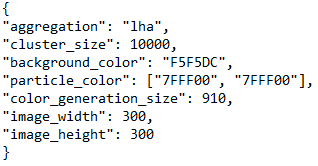
\includegraphics[height=3.33cm]{images/code-snippets/parameters.png} \\
\\
The value $\mathit{color\_generation\_size}$ specifies how big one generation of a color shall be in the case that we choose more than one color to print the particles. So if we for example enter the values $["000000","\text{ff0000}","\text{ffffff}"]$ for $"particle\_color"$ and $100$ for $"color\_generation\_size"$, then the first 100 particles will be printed in color $"000000"$ (black), the next 100 in $"\text{ff}0000"$ (red), the next in $"\text{ffffff}"$ (white) and the next back again in black, and so on. This allows to visualize layers of the aggregation and produce beautiful rainbowlike colored realizations. Since for the simulation here we only use black particle color, the color generation size does not have any effect in this case. With the $\mathit{fractal\_calculation\_range}$ we can have influence on how the approximation of the fractal dimension shall be calculated, more on that later. We can find more about setting parameters in the README file of the repository. \\

\noindent If correct parameters are set, we can run a shell script which in turn will run a single python file $\mathit{main.py}$ which reads the entered parameters and executes first the mathematical process which needs the mathematical imports and second the data creation of the calculated process which needs the systemic imports as described above. The created data will contain an image of the created cluster, a json file with the parameters saved for later lookup and another json file containing information about the creation time, fractal dimension values and a list of all particle coordinates for potential later use. \\
\\We will have a look now on what happens on the mathematical side. We will show code directly here to make things clearer. Note that in the original code here and there we will find comments or other irrelevant differences, which we leave away here. \\
\\The main executed python file $\mathit{main.py}$ looks like this:\\
\\
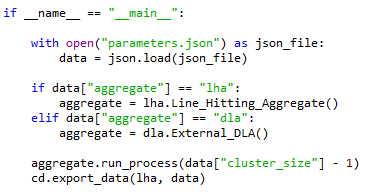
\includegraphics[height=4.66cm]{images/code-snippets/mainpy.png} \\
\\
Note again that we can also run an external DLA simulation but we do not claim that it is mathematically precise and therefore we do not discuss it here. The parameters in $\mathit{parameters.json}$ are read and depending on which process (LHA or DLA) shall be simulated, the according object gets initiated and its $\mathit{run\_process}$ method gets executed. Both classes $\mathit{Line\_Hitting\_Aggregation}$ and $\mathit{External\_DLA}$ base on the class $\mathit{Incremental\_Aggregation}$. So the full initialization of LHA looks like: \\
\\
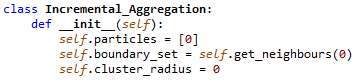
\includegraphics[height=1.8cm]{images/code-snippets/initia.png} \\
\\
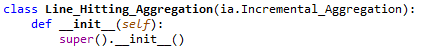
\includegraphics[height=1.1cm]{images/code-snippets/lhainit.png} \\
\\
We initialize the particle set $\mathit{particles}$ as a set containing $0$, initialize the boundary set which in every iteration of the process will contain all neighbours of all particles in the particle set that are not in the particle set themselves and set the initial cluster radius to $0$. As neighbours we only consider graph neighbours (up, down, left and right) as defined in \ref{zgraph}. \\
\\After initializing a $\mathit{Line\_Hitting\_Aggregation}$ object the method $\mathit{run\_process}$ gets executed, which reads as follows: \\
\\
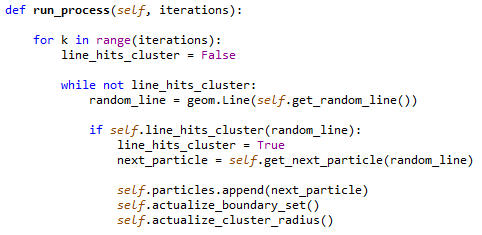
\includegraphics[height=5cm]{images/code-snippets/runprocess.png} \\
\\
This method will directly run a loop with $\mathit{data["cluster\_size"] - 1}$ iterations. In each iteration exactly one particle will be added to the particle set, so that we end up with exactly $\mathit{data["cluster\_size"]}$ particles since we started with one particle. \\
\\If we call $K$ the current cluster it is now important to recall again, how choosing random $K$-isotropic lines works. In \ref{choosekiso} we have argued that a $K$-isotropic line can be realized by considering a ball $B$ which contains the current cluster $K$ and choose a $B$-isotropic line. If it happens that this line intersects with $K$ then, by \ref{circ}, we know that we have realized a random $K$-isotropic line. The method $\mathit{get\_random\_line}$ \\
\\
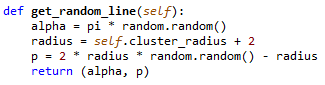
\includegraphics[height=1.8cm]{images/code-snippets/randomline.png} \\
\\
produces a uniformly chosen pair of line parameters$(\alpha,p)$, and using $\mathit{cluster\_radius + 2}$ here ensures that the resulting ball $B$ does contain the cluster. The method $\mathit{random.random()}$ produces an uniformly chosen value in $[0,1)$. The fact that $\mathit{random.random()}$ cannot choose the value $1$ doesn't disturb the distribution of the line since $\{1\}$ is a zero set for the $1$-dimensional Lebesgue-measure. By \ref{chi}, choosing these line parameters uniformly indeed realizes a random $B$-isotropic line. \\
\\After having realized a $B$-isotropic line by choosing its line parameters as described above, we want to check whether the line hits the cluster or not which is implemented in the method $\mathit{line\_hits\_cluster}$. \\
\\
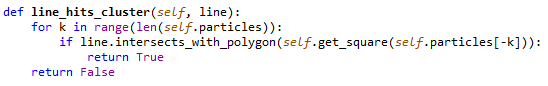
\includegraphics[height=1.8cm]{images/code-snippets/linehitscluster.png} \\
\\
This method bases on the method $\mathit{intersects\_with\_polygon}$ which evaluates whether a line intersects with a given general polygon or not (the implemented geometry classes $\mathit{Line}$ and $\mathit{Polygon}$ we can find in the file $\mathit{geometry.py}$). Here the polygon is a square given by the method \\
\\
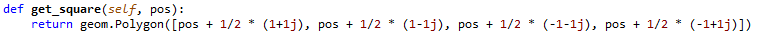
\includegraphics[height=0.8cm]{images/code-snippets/getsquare.png} \\
\\
which implements the Definitions \ref{squares} and \ref{ghitA}. \\
\\If the condition is satisfied that a chosen line hits the cluster, we enter the if-condition and then choose the next particle with the method $\mathit{get\_next\_particle}$\\
\\
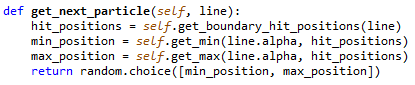
\includegraphics[height=1.8cm]{images/code-snippets/nextparticle.png} \\
\\
which first collects all particle squares in the boundary set which are hit by the line, calculates minimum and maximum of all those particles and then chooses uniformly between minimum and maximum with $\mathit{random.choice}$. The methods $\mathit{get\_min}$ and $\mathit{get\_max}$ base on the method $\mathit{is\_lower}$\\
\\
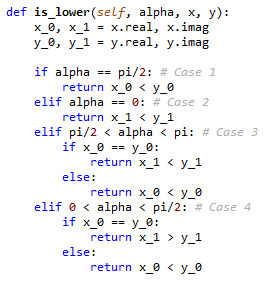
\includegraphics[height=6cm]{images/code-snippets/islower.png} \\
\\
which implements the totally ordered relation on all squares which got hit by the line as defined in \ref{ghitA}. Minimum and maximum are then canonically calculated with respect to this relation. \\
\\After having realized the next particle, values like the particle set, the boundary set and the cluster radius get updated and the next iteration starts. When all iterations are calculated, data like the image, the informations file and a copy of the parameters file are created which can be found in the folder $\mathit{exports}$. In the image file we can see the process printed in the colors we have specified in the parameters file. In the information file we can find date and time when the simulation was run, the running time of the simulation in seconds, the linear regression parameters, the last fractal dimension value and volume ratio as described in the next section, and finally the whole list of particles of the process for later use. \\
\\In the next section we look at some empirical values of LHA. 


\subsection{Empirical values of LHA}

In this section we present what our simulations produce in terms of images and fractal dimension values. Since by Theorem \ref{2theorem} we already know that the fractal dimension of line hitting aggregation is $2$, our approximation for the fractal dimension here has the purpose to give an idea of the convergence behaviour towards the value $2$. First it is worth to mention that it is not trivial to create a senseful approximation for the fractal dimension. If we go back to the definition 
\begin{flalign*}
	d_f = \lim_{n\to\infty} \frac{\ln(n)}{\ln(\rad(\E_n))}
\end{flalign*}
we can start with the ansatz that 
\begin{flalign*}
	\rad(\E_n) \approx c n^{\frac{1}{d_f}}
\end{flalign*}
for some constant $c>0$ and therefore get 
\begin{flalign} \label{linearplot}
	\ln(\rad(\E_n)) \approx \frac{1}{d_f} \ln(n) + \ln(c). 
\end{flalign}
Therefore we could be looking for the parameters $\frac{1}{d_f}$ and $\ln(c)$ of a linear regression of the two values $\ln(n)$ and $\ln(\rad(\E_n))$ for a range of values $n\in\{1,\dots,m\}$, $m\in\N$. In the range of up to 100000 particles we have noticed a strong instability of these parameters as functions of the maximum value $m$. We have come to the conclusion that for calculating approximations it is problematic that the radius of a cluster always stays constant for the time that new particles get added to the cluster where they don't increase the radius. Compare with \autoref{notfilled} and the discussion in Remark \ref{altdim} to see that this cluster is not yet \glqq filled up\grqq\ to its radius which creates something like a stair function in the linear plot of \ref{linearplot}. \\

\noindent To get more stable parameters it makes sense to come back to Remark \ref{finfty} and write
\begin{flalign*}
	d_f = d_\infty = \lim_{n\to\infty} \frac{\ln(|\E_\infty \cap B_n|)}{\ln(n)}.
\end{flalign*}
With the ansatz
\begin{flalign} \label{ansatz}
	 |\E_\infty \cap B_n| \approx c_1 n^{d_f}
\end{flalign}
for some constant $c_1>0$ we would get 
\begin{flalign} \label{newlinreg}
	\ln(|\E_\infty \cap B_n|) \approx d_f \ln(n) + \ln(c_1). 
\end{flalign}

\begin{figure}[t]
	\begin{subfigure}[b]{.31\textwidth}
		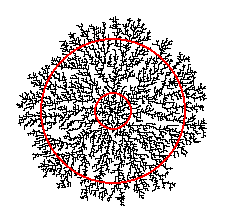
\includegraphics[width=1\linewidth]{images/fractal_range/1.PNG}
	\end{subfigure}
	\begin{subfigure}[b]{.31\textwidth}
		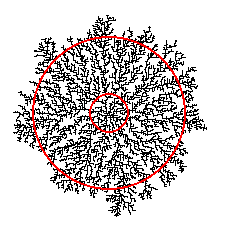
\includegraphics[width=1\linewidth]{images/fractal_range/4.PNG}
	\end{subfigure}
	\begin{subfigure}[b]{.31\textwidth}
		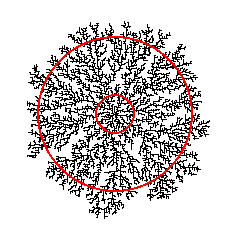
\includegraphics[width=1\linewidth]{images/fractal_range/2.PNG}
	\end{subfigure}
	\caption{circle radii range [0.2, 0.75] of the clusters radius}
	\label{filledup}
\end{figure}

Recall that $\E_\infty \cap B_n$ is the set of all particles of the limit cluster $\E_\infty$ which lie in $B_n$, the ball with radius $n$ and center $0$. Since it is not possible to realize $\E_\infty$, we have to use an approximation here. What we want to compare is the particle number of \glqq filled up\grqq\ clusters with their radius. If we have a look at \autoref{filledup} and let $r$ be the radius of the cluster in the figure, then we can see that in a certain range of radii $n\in[ar,br]$ with values $0\leq a< b \leq 1$ the clusters $\E_\infty \cap B_n$ seem to be fairly filled up (this range is described with the two red circles). This range of radii is what can be specified in the $\mathit{parameters.json}$ file in the $\mathit{fractal\_calculation\_range}$ field (see in the git repository). We found that it makes sense to not start the observation at $0$ but a bit higher like $a=0.2$ to avoid distorted values occuring by the beginning of the process. On the other side we found empirically that $b=0.75$ seems to be a fair upper ratio where the clusters in most cases seem to be fairly filled up. Note that in the parameters file we should enter the values $a$ and $b$, not $ar$ and $br$. So a correct setting would be $[0.2,0.75]$.  \\
\\So all in all we will look at radii in the specified range $n\in[0.2r, 0.75r]$ and count all particles of the cluster which lie in $B_n$, which shall be an approximation of $|\E_\infty \cap B_n|$. After that we calculate the linear regression parameters $\hat d_f$ and $\hat c_1$ for $d_f$ and $\ln(c_1)$, respectively, as described in (\ref{newlinreg}) which happens in the following method:\\
\\
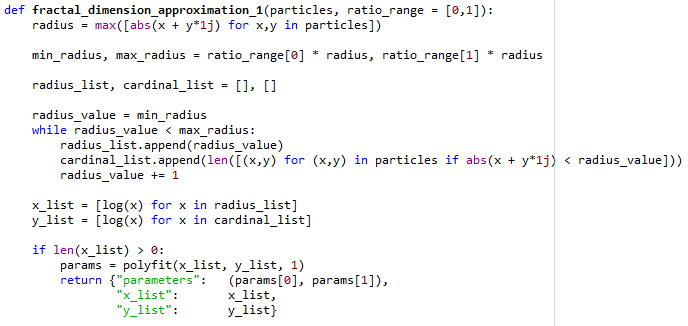
\includegraphics[height=7.5cm]{images/code-snippets/fractalnew.png} \\
\\
We will find every of the following realized simulations in the folder $\mathit{exports}$ of the git repository. Inside a folder we will find three types of files, one is the created image, one contains information about the process as described at the end of the last section and the third is a copy of the parameters file the simulation was preset with. More on that we can find in the README file of the repository. The names of the folder and files will have a certain format to identify each simulation clearly. The folder name
\begin{flalign*}
	\text{2021\_03\_02\_02\_37\_54\_\_lha\_100000}
\end{flalign*}
indicates that the folder contains a realized LHA simulation with 100000 particles which was created at 02. March 2021 02:37:54. Analogously 
\begin{flalign*}
	\text{2021\_03\_02\_11\_02\_25\_\_dla\_5000}
\end{flalign*}
is the folder of a realized simulation of DLA. For the following observation we have run line hitting aggregation from 10000 to 100000 twice at each 10000 step which makes 20 simulations in total. The simulations have produced the values in \autoref{lhasimulation}. A plot of the values can be found in \autoref{plot}. The plot indicates a rather slow convergence of the empirical dimension values towards the theoretical value $2$. Something similar was guessed by \cite{ballistic}. For a further empirical study on this convergence behaviour more simulations would be necessary. \\

\begin{table}[t]
	\centering
	\begin{tabular}{llll}
		$\mathbf{Simulation\ name}$                       & $\hat d_f\ (d_f)$   & $\hat c_1\ (\ln(c_1))$   & $\hat c_v\ (c_v)$\\
		\hline
		2021\_03\_04\_09\_40\_51\_\_lha\_10000  & 1.8601 & 0.8083 & 0.4198\\
		2021\_03\_04\_10\_05\_53\_\_lha\_10000  & 1.8679 & 0.7847 & 0.4222\\
		2021\_03\_04\_11\_53\_34\_\_lha\_20000  & 1.9135 & 0.5899 & 0.4006\\
		2021\_03\_04\_12\_35\_01\_\_lha\_20000  & 1.9273 & 0.5265 & 0.3976\\
		2021\_03\_04\_13\_54\_14\_\_lha\_30000  & 1.9071 & 0.6370 & 0.4016\\
		2021\_03\_04\_14\_49\_08\_\_lha\_30000  & 1.9191 & 0.5734 & 0.3965\\
		2021\_03\_04\_15\_56\_37\_\_lha\_40000  & 1.9518 & 0.4164 & 0.3885\\
		2021\_03\_04\_18\_00\_02\_\_lha\_40000  & 1.9173 & 0.5874 & 0.3941\\
		2021\_03\_04\_15\_58\_28\_\_lha\_50000  & 1.9311 & 0.5127 & 0.3863\\
		2021\_03\_04\_18\_00\_18\_\_lha\_50000  & 1.9381 & 0.4664 & 0.3811\\
		2021\_03\_04\_12\_35\_20\_\_lha\_60000  & 1.9283 & 0.5328 & 0.3868\\
		2021\_03\_04\_09\_42\_12\_\_lha\_60000  & 1.9187 & 0.5771 & 0.3861\\
		2021\_03\_04\_09\_42\_36\_\_lha\_70000  & 1.9257 & 0.5467 & 0.3853\\
		2021\_03\_04\_13\_43\_38\_\_lha\_70000  & 1.9184 & 0.5707 & 0.3812\\
		2021\_03\_04\_09\_42\_56\_\_lha\_80000  & 1.9135 & 0.6230 & 0.3906\\
		2021\_03\_04\_14\_49\_16\_\_lha\_80000  & 1.9463 & 0.4352 & 0.3788\\
		2021\_03\_04\_16\_30\_00\_\_lha\_90000  & 1.9420 & 0.4632 & 0.3805\\
		2021\_03\_04\_09\_43\_16\_\_lha\_90000  & 1.9344 & 0.5083 & 0.3834\\
		2021\_03\_03\_21\_23\_50\_\_lha\_100000 & 1.9065 & 0.6421 & 0.3805\\
		2021\_03\_03\_21\_23\_47\_\_lha\_100000 & 1.9344 & 0.4989 & 0.3782
	\end{tabular}
	\caption{LHA Simulations (10000 - 100000 particles)}
	\label{lhasimulation}
\end{table}

\begin{figure}[h]
	\centering
	\begin{subfigure}[b]{.45\textwidth}
		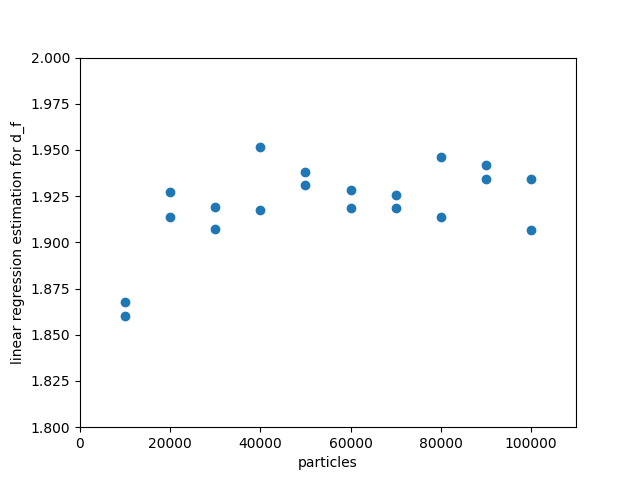
\includegraphics[width=1\linewidth]{images/lhaplot.png}
	\end{subfigure}
	\begin{subfigure}[b]{.45\textwidth}
		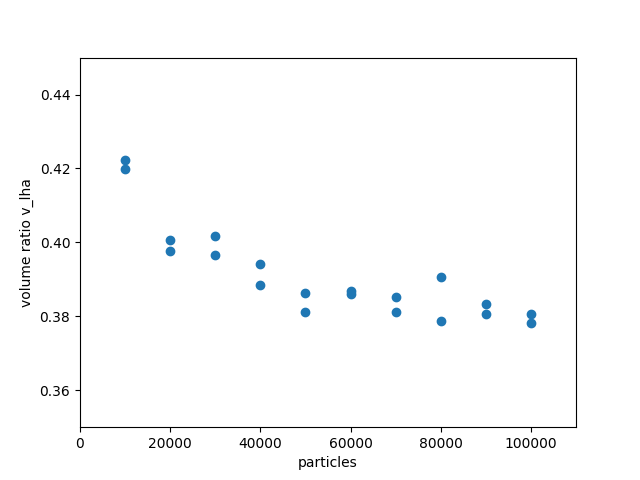
\includegraphics[width=1\linewidth]{images/volumeplot.png}
	\end{subfigure}
 \caption{Linear regression parameters and volume ratio of LHA}
 \label{plot}
\end{figure}

Another interesting value to calculate is the following. Since we know that the fractal dimension for LHA is $2$, we can rewrite (\ref{ansatz}) to get
\begin{flalign} \label{ansatz2}
	|\E_\infty \cap B_n| \approx c_2 n^2 
\end{flalign}
for some constant $c_2>0$ which can be transformed to
\begin{flalign*}
	\frac{c_2}{\pi} \approx \frac{|\E_\infty \cap B_n|}{\pi n^2}.
\end{flalign*}
We can see that $\frac{c_2}{\pi}$ describes the relation between the volume of the cluster in the ball $B_n$ and the volume of the ball $B_n$ itself. Hence $\frac{c_2}{\pi}$ can be interpreted as the $\mathit{volume}$ $\mathit{fraction}$ of the limit cluster $\E_\infty$ which can be formally defined as
\begin{flalign*}
	c_v := \lim_{n\to\infty} \frac{|\E_\infty \cap B_n|}{\pi n^2},
\end{flalign*}
if the limit exists. If we look at the ansatz
\begin{flalign} \label{newlinreg2}
	\ln(|\E_\infty \cap B_n|) \approx 2 \ln(n) + \ln(c_2)
\end{flalign}
similar to linear regression we can calculate an in the sense of a minimal quadratic error optimal estimator $\hat c_2$ for $\ln(c_2)$ which satisfies
\begin{flalign*}
	\hat c_2 = \underset{c\in\R}{\text{argmin}} \sum_{n = m_1}^{m_2} (\ln(|\E_\infty \cap B_n|) - (2 \ln(n) + c))^2,
\end{flalign*}
where $m_1 := \min ([0.2r, 0.75r] \cap \N)$ and $m_2:=\max ([0.2r, 0.75r] \cap \N)$. It is not difficult to show that $\hat c_2$ is given by
\begin{flalign*}
	\hat c_2 = \frac{1}{m_2-m_1+1} \sum_{n = m_1}^{m_2} \ln(|\E_\infty \cap B_n|) - 2 \ln(n). 
\end{flalign*}
We can then obtain an estimator $\hat c_v$ for the volume ratio $c_v$ via
\begin{flalign*}
	\hat c_v := \frac{e^{\hat c_2}}{\pi}.
\end{flalign*}
In \autoref{lhasimulation} we can find the values for $\hat c_v$ which have been produced by our simulations. \autoref{plot} indicates that the volume ratio decreases as the number of particles grows and possibly starts to stabilize at around $c_v \approx 0.38$. For a further study on the volume ratio again more simulations would be necessary. 


\newpage
\phantom \\
\newpage
\subsection{Images}
In the following we present some of the realized images of our LHA and external DLA simulations. More can be found in the repository in the folder $\mathit{exports}$.

\begin{figure}[h!]
	\centering
	\begin{subfigure}[b]{.49\textwidth}
		\centerline{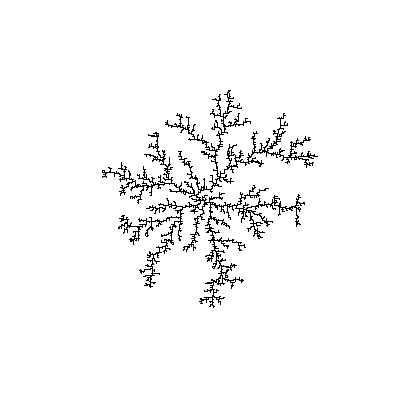
\includegraphics[height=7cm]{images/ia/2021_03_03_12_25_49__image_dla_5000.png}}
		\captionsetup{labelformat=empty}
		\caption{2021\_03\_03\_12\_25\_49\_\_image\_dla\_5000.png}
	\end{subfigure}
	\begin{subfigure}[b]{.49\textwidth}
		\centerline{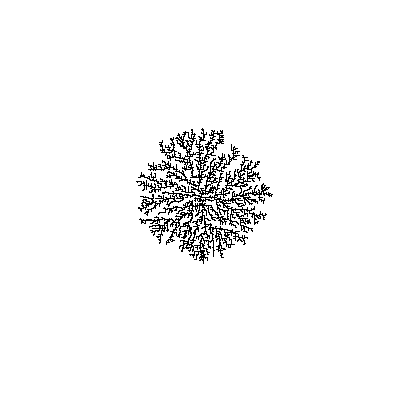
\includegraphics[height=7cm]{images/ia/2021_03_06_00_23_38__image_lha_5000.png}}
		\captionsetup{labelformat=empty}
		\caption{2021\_03\_06\_00\_23\_38\_\_image\_lha\_5000.png}
	\end{subfigure}
\end{figure}

\begin{figure}[h!]
	\centering
	\begin{subfigure}[b]{.49\textwidth}
		\centerline{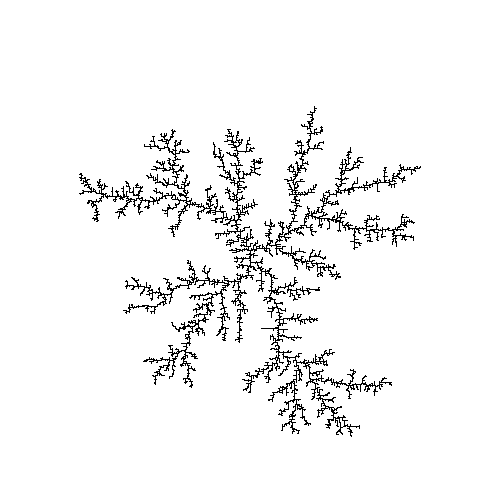
\includegraphics[height=8.75cm]{images/ia/2021_03_03_19_58_26__image_dla_10000.png}}
		\captionsetup{labelformat=empty}
		\caption{2021\_03\_03\_19\_58\_26\_\_image\_dla\_10000.png}
	\end{subfigure}
	\begin{subfigure}[b]{.49\textwidth}
		\centerline{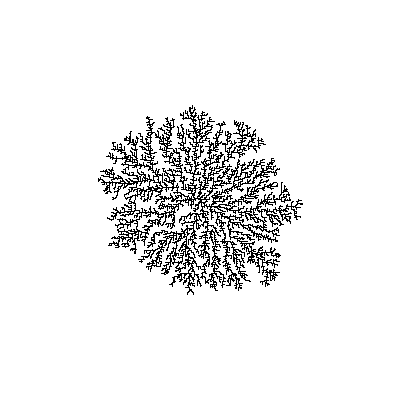
\includegraphics[height=7cm]{images/ia/2021_03_05_23_28_53__image_lha_10000.png}}
		\captionsetup{labelformat=empty}
		\caption{2021\_03\_05\_23\_28\_53\_\_image\_lha\_10000.png}
	\end{subfigure}
\end{figure}

\begin{figure}[p]
	\centering
	\begin{subfigure}[]{0.48\textwidth}
		\centerline{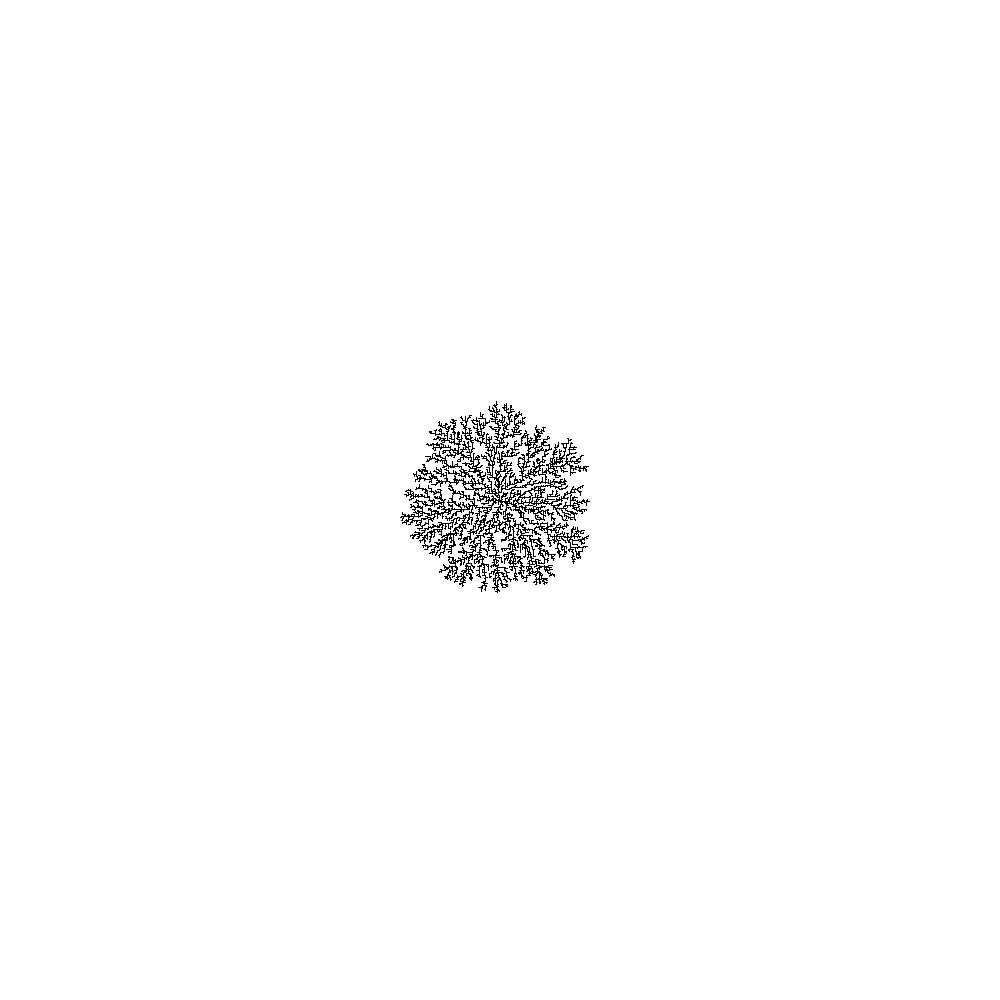
\includegraphics[height=9.5cm]{images/ia/2021_03_04_10_05_53__image_lha_10000.png}}
		\captionsetup{labelformat=empty}
		\caption{2021\_03\_04\_10\_05\_53\_\_image\_lha\_10000.png} 
	\end{subfigure}
	\begin{subfigure}[]{0.48\textwidth}
		\centerline{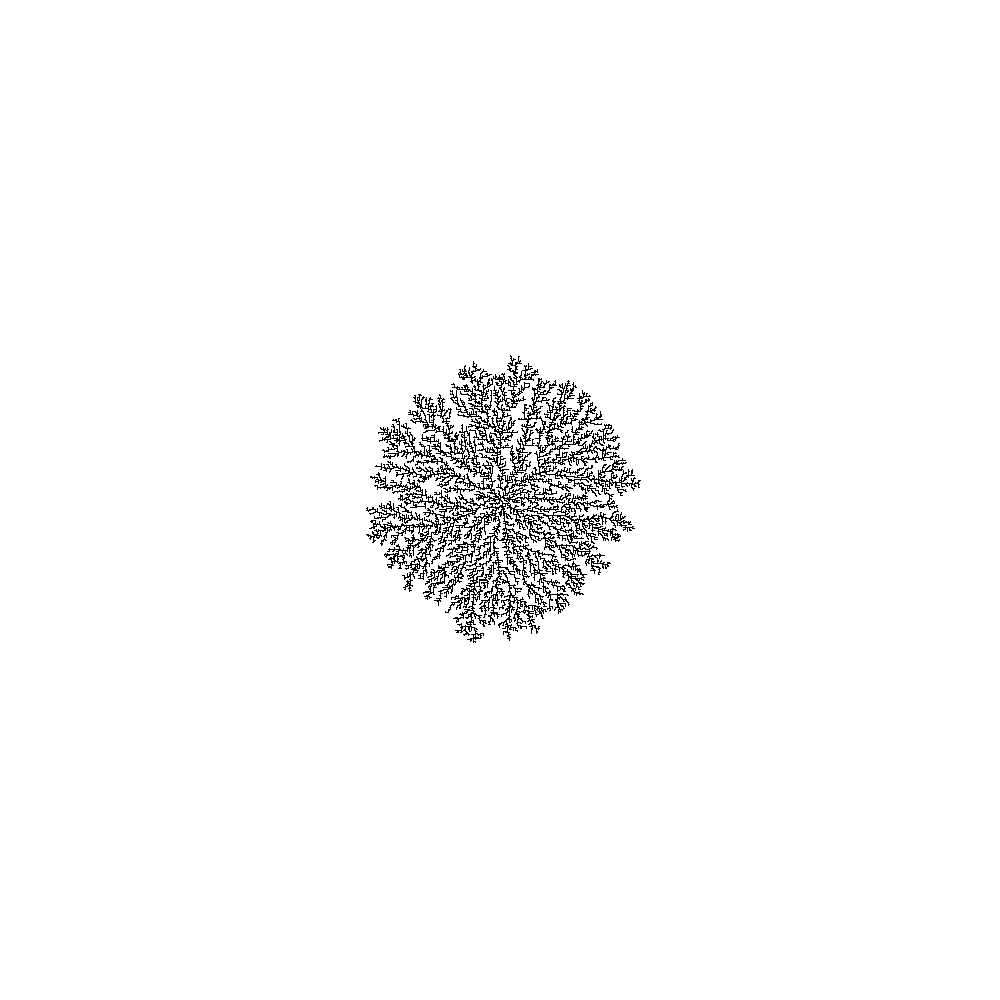
\includegraphics[height=9.5cm]{images/ia/2021_03_04_11_53_34__image_lha_20000.png}}
		\captionsetup{labelformat=empty}
		\caption{2021\_03\_04\_11\_53\_34\_\_image\_lha\_20000.png} 
	\end{subfigure}
\end{figure}

\begin{figure}[]
	\centering
	\begin{subfigure}[]{0.48\textwidth}
		\centerline{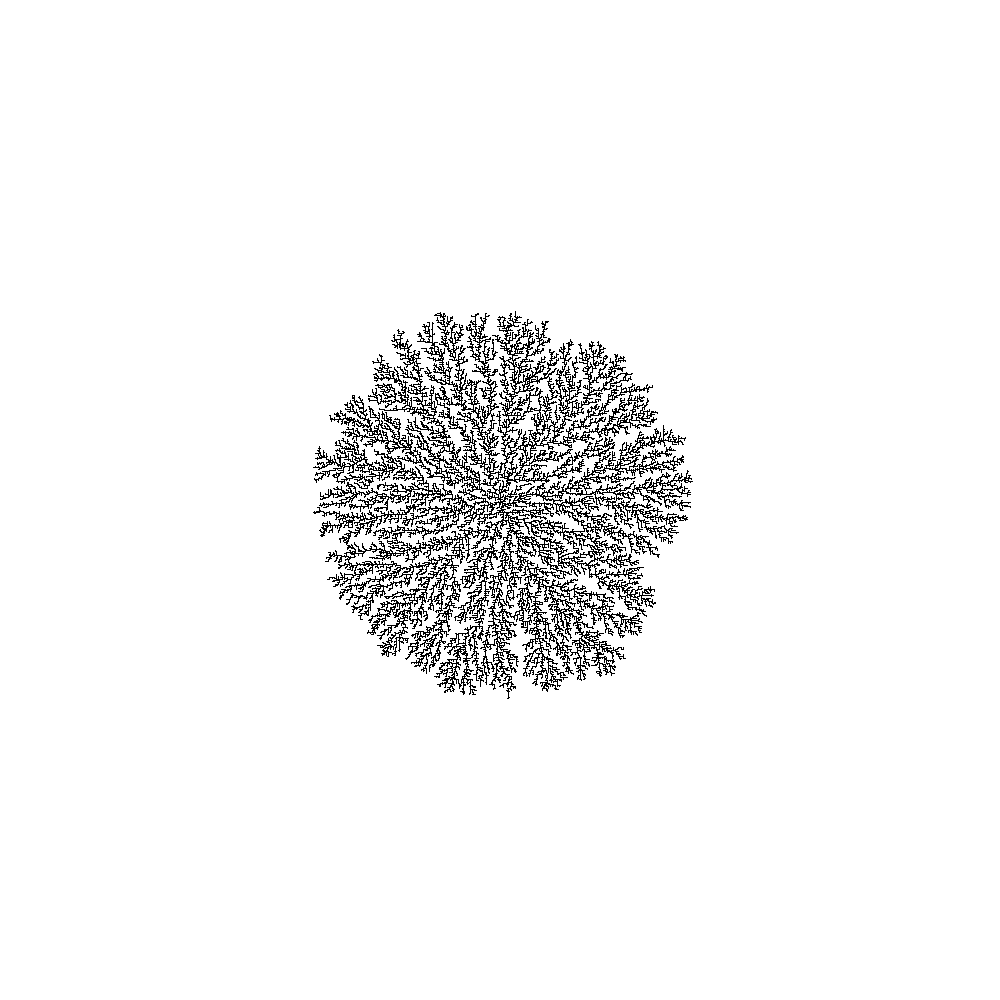
\includegraphics[height=9.5cm]{images/ia/2021_03_04_18_00_02__image_lha_40000.png}}
		\captionsetup{labelformat=empty}
		\caption{2021\_03\_04\_18\_00\_02\_\_image\_lha\_40000.png} 
	\end{subfigure}
	\begin{subfigure}[]{0.48\textwidth}
		\centerline{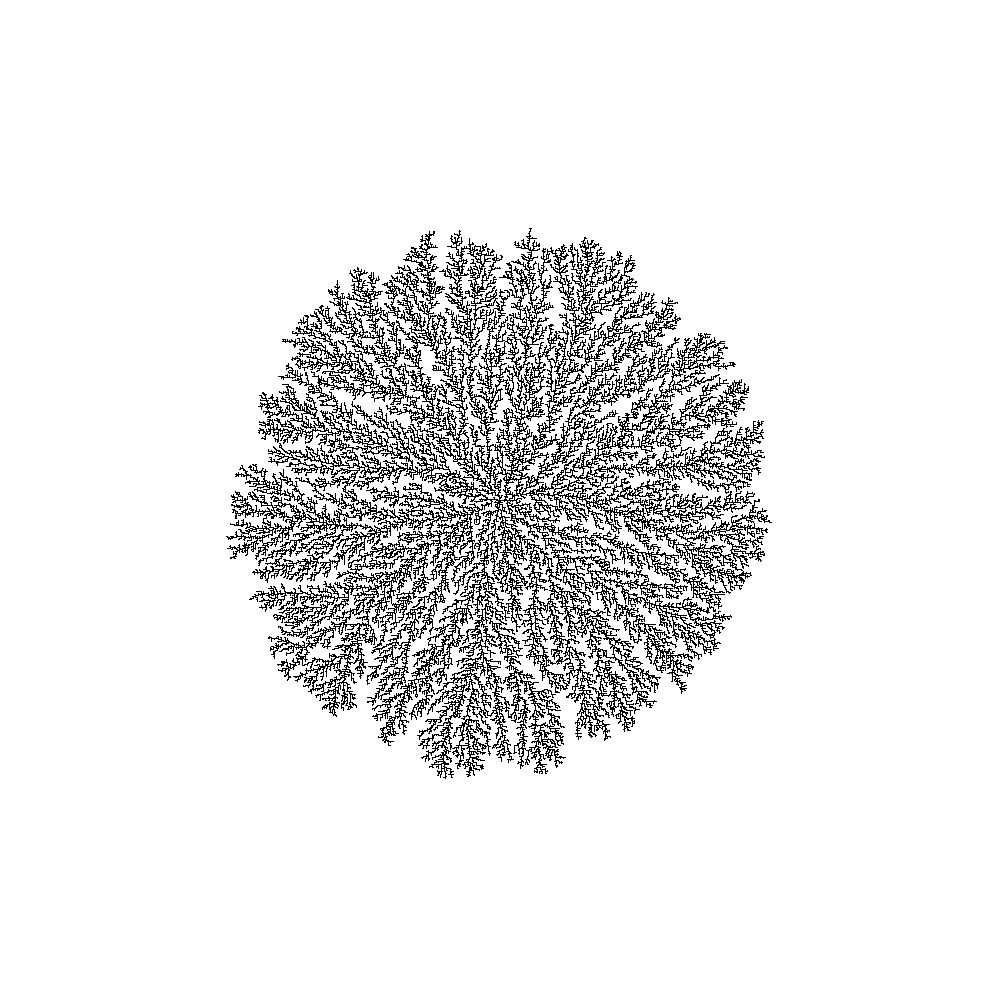
\includegraphics[height=9.5cm]{images/ia/2021_03_04_09_42_56__image_lha_80000.png}}
		\captionsetup{labelformat=empty}
		\caption{2021\_03\_04\_09\_42\_56\_\_image\_lha\_80000.png} 
	\end{subfigure}
\end{figure}



\begin{figure}[p]
	\centering
	\centerline{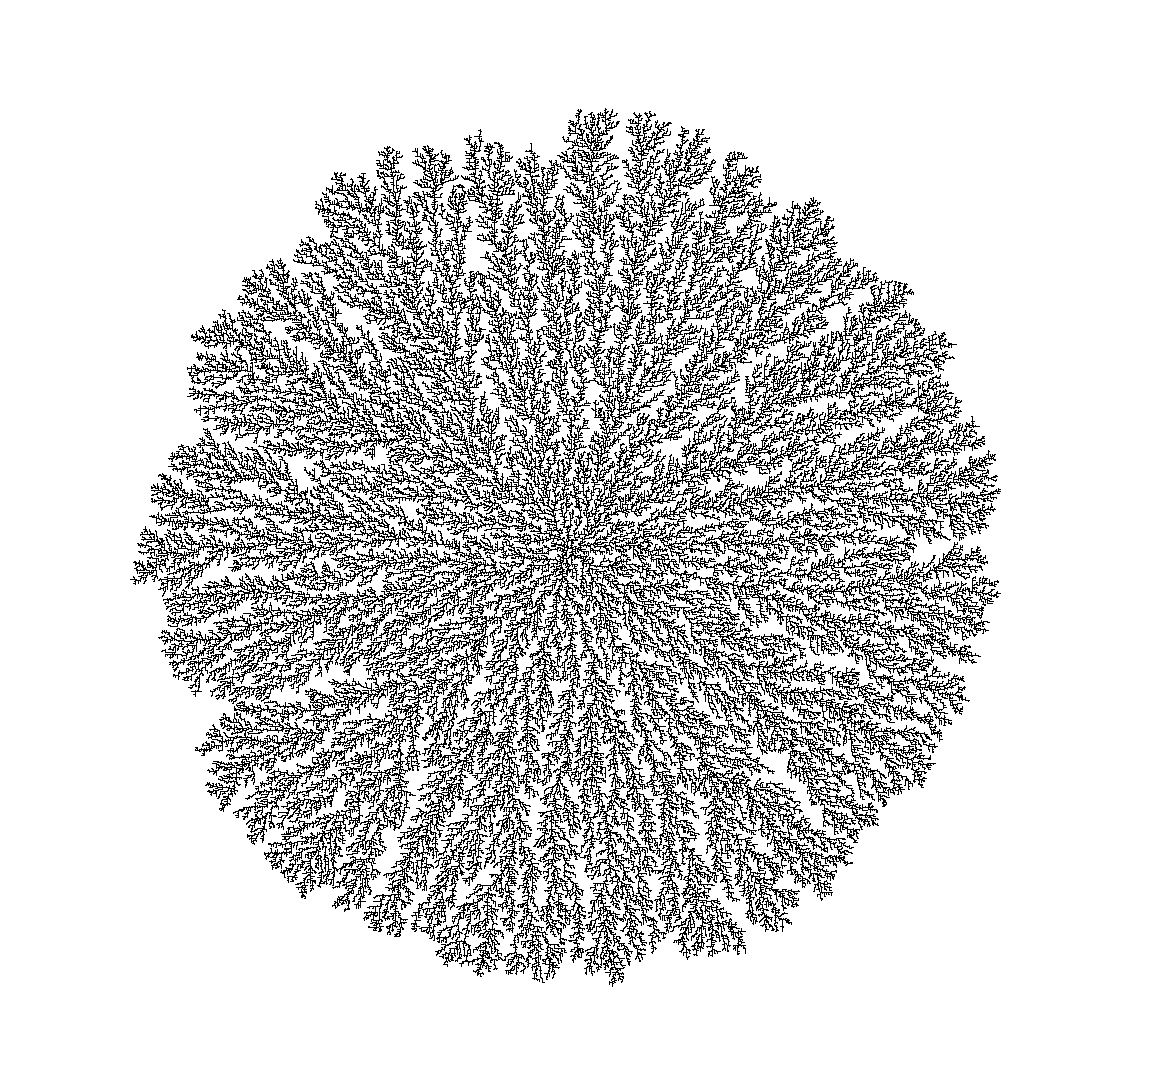
\includegraphics[height=21cm]{images/ia/2021_03_04_00_42_19__image_lha_200000.png}}
	\captionsetup{labelformat=empty}
	\caption{2021\_03\_04\_00\_42\_19\_\_image\_lha\_200000.png}
\end{figure}


\newpage

\begin{figure}[h!]
	\centering
	\begin{subfigure}[b]{.49\textwidth}
		\centerline{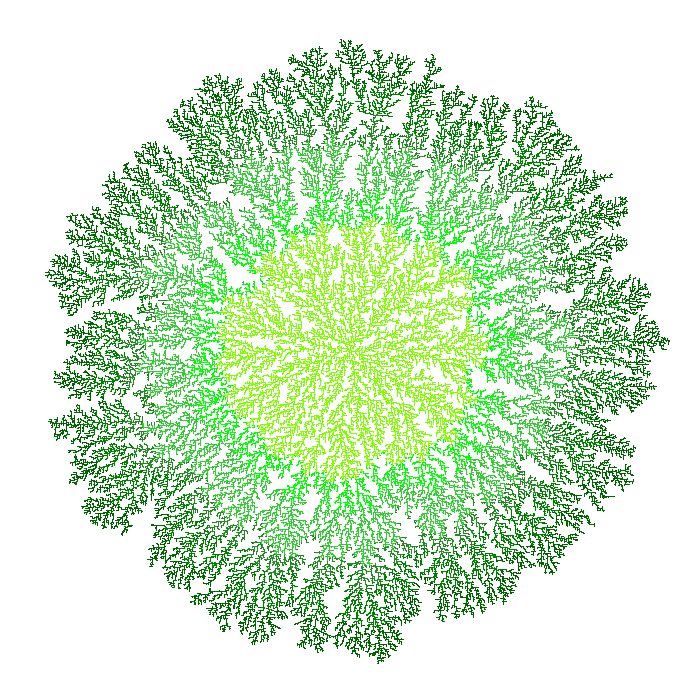
\includegraphics[height=8cm]{images/ia/2021_03_03_21_23_50___100000__10000__8923.png}}
		\captionsetup{labelformat=empty}
		\caption{2021\_03\_03\_21\_23\_50\_\_lha\_100000, green, color generation size of 10000}
	\end{subfigure}
	\begin{subfigure}[b]{.49\textwidth}
		\centerline{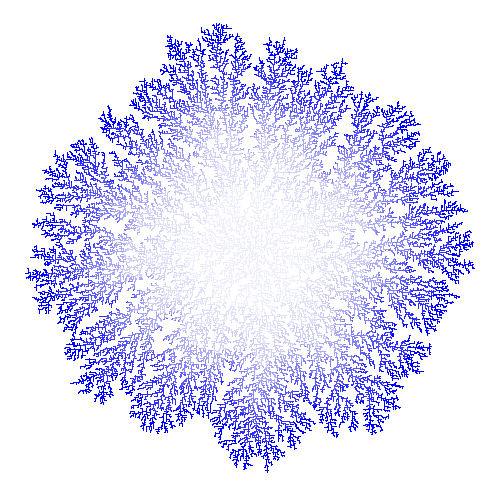
\includegraphics[height=8cm]{images/ia/2021_03_04_15_58_28___50000__5000__5250.png}}
		\captionsetup{labelformat=empty}
		\caption{2021\_03\_04\_15\_58\_28\_\_lha\_50000, rising blue, color generation size of 5000}
	\end{subfigure}
\end{figure}

\vspace*{\fill}

\begin{figure}[h!]
	\centering
	\begin{subfigure}[b]{.49\textwidth}
		\centerline{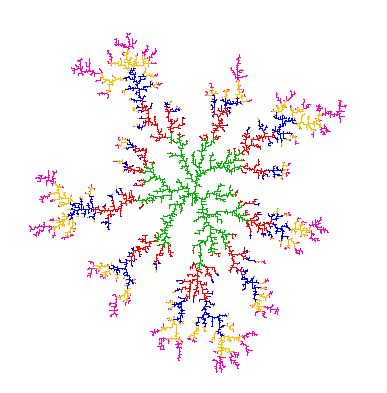
\includegraphics[height=8cm]{images/ia/2021_03_03_19_59_39___10000__2000__7448.png}}
		\captionsetup{labelformat=empty}
		\caption{2021\_03\_03\_19\_59\_39\_\_dla\_10000, \\five colors , color generation size of 2000}
	\end{subfigure}
	\begin{subfigure}[b]{.49\textwidth}
		\centerline{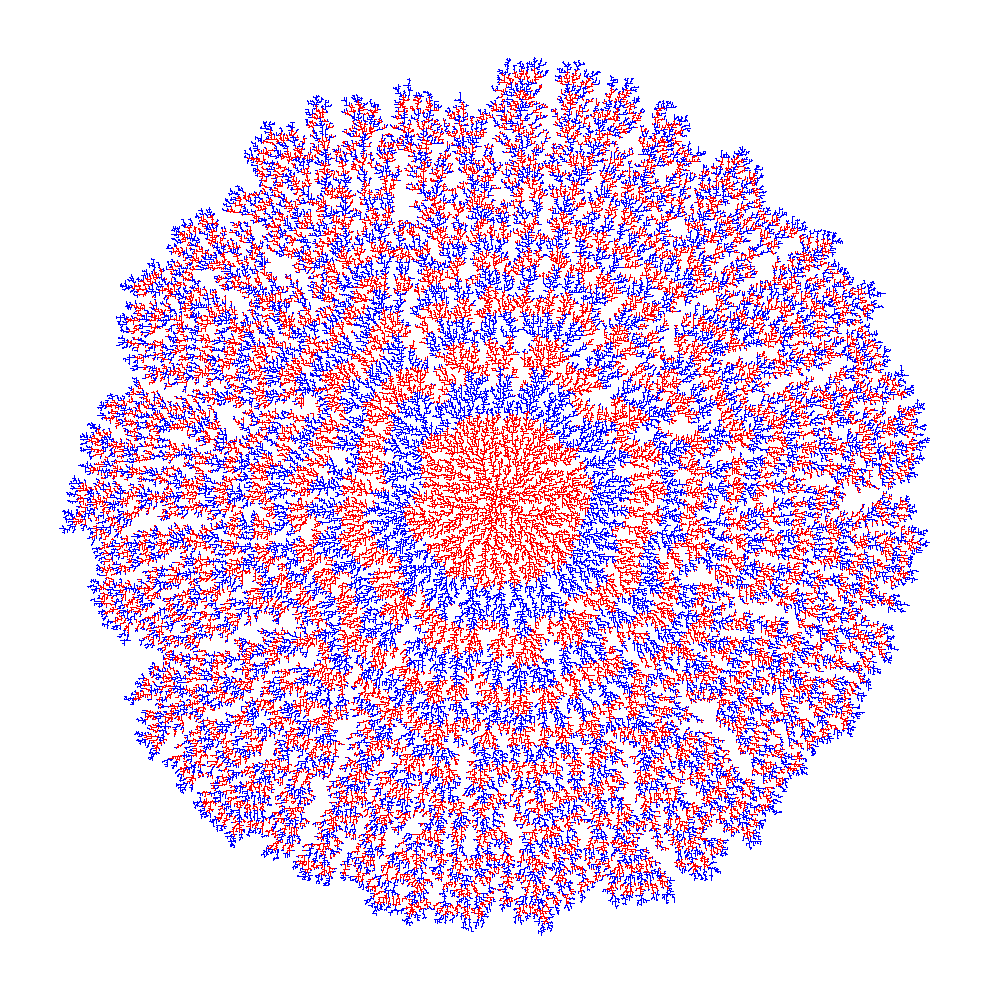
\includegraphics[height=8cm]{images/ia/2021_03_04_00_42_19___200000__10000__6945.png}}
		\captionsetup{labelformat=empty}
		\caption{2021\_03\_04\_00\_42\_19\_\_lha\_200000, \\dual color, color generation size of 10000}
	\end{subfigure}
\end{figure}



\begin{figure}[p]
	\centering
	\begin{subfigure}[]{0.77\textwidth}
		%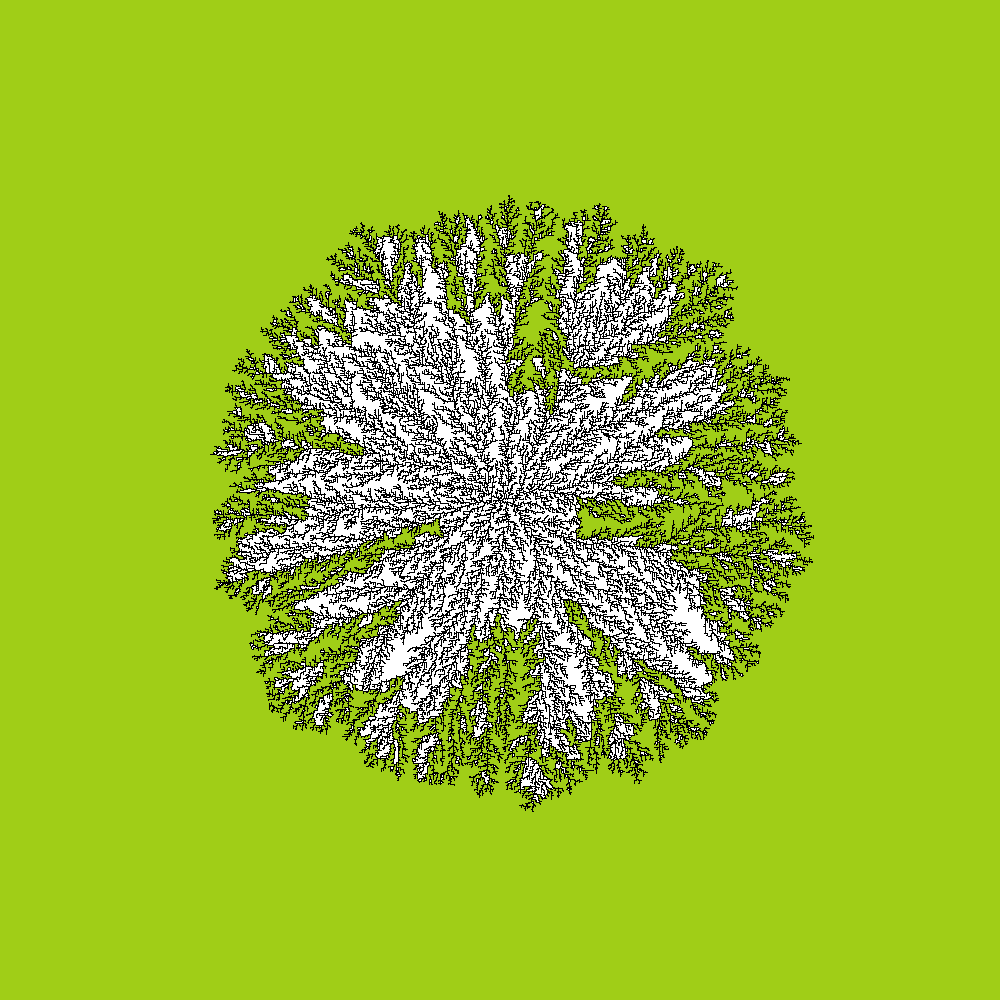
\includegraphics[width=1\linewidth]{images/ia/2021_03_03_21_23_47__image_lha_100000 - colored.png}
		\centerline{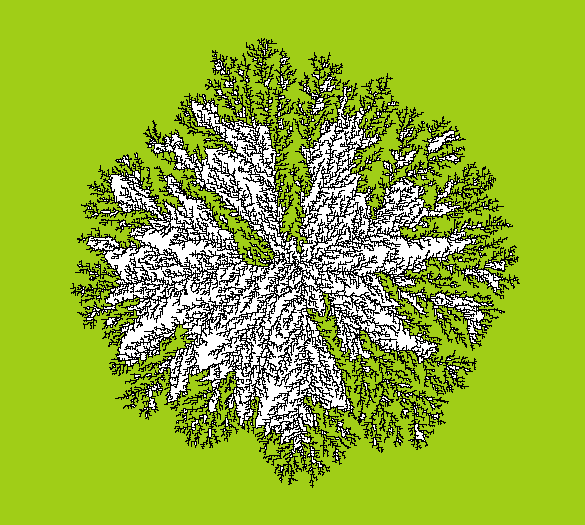
\includegraphics[width=1\linewidth]{images/ia/2021_03_04_15_58_28__lha_50000_colored.png}}
		\captionsetup{labelformat=empty}
		\caption{2021\_03\_04\_15\_58\_28\_\_lha\_50000 colored from outside} 
	\end{subfigure}
	\begin{subfigure}[]{0.77\textwidth}
		\centerline{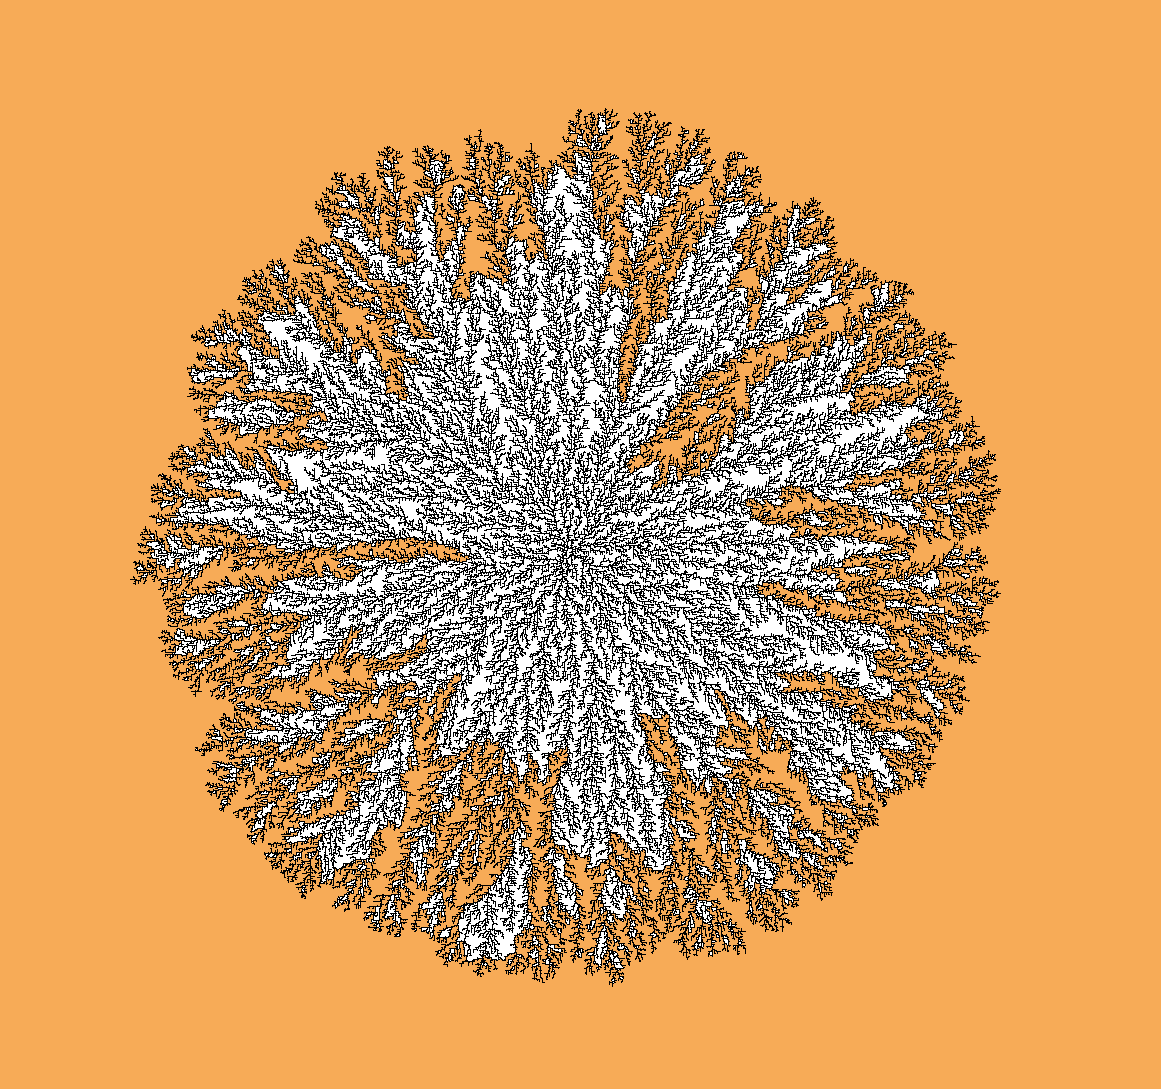
\includegraphics[width=1\linewidth]{images/ia/2021_03_04_00_42_19__lha_200000_colored.png}}
		\captionsetup{labelformat=empty}
		\caption{2021\_03\_04\_00\_42\_19\_\_lha\_200000 colored from outside} 
	\end{subfigure}
\end{figure}




\newpage
\phantom \\
\newpage

\section{Review}
In this paper we have looked at a general definition of incremental aggregations in $\Z^d$ and the notion of a fractal dimension of such discrete random clusters. In Theorem \ref{iatheorem} we found a condition for proving a lower bound of the fractal dimension. We where able to apply this theorem for the $2$-dimensional case of both incremental aggregations we looked at in this paper, external diffusion limited aggregation (external DLA) and line hitting aggregation (LHA). In $\Z^2$, for external DLA we found a lower bound of 
\begin{flalign*}
	d_f^{dla} \geq \frac{3}{2}\quad\text{a.s.}
\end{flalign*}
and for line hitting aggregation we were even able to find the exact dimension, which is
\begin{flalign*}
	d_f^{lha} = 2 \quad\text{a.s.}.
\end{flalign*}
In the last chapter we provided simulations for both incremental aggregations. Especially the one for LHA was implemented as close to its mathematical definition as possible. \\
\\All in all did we here only touch the properties of incremental aggregations. The most known such model we can find in literature is probably external DLA, but the general definition here in this paper opens a door to other interesting incremental aggregations. \\
\\I hope that I could raise interest in this topic through my work in this paper and I invite the reader to play around with the code I provided in a github repository (see at the beginning of Chapter \ref{simulation}). I feel delighted when looking at the beautiful realizations of the aggregations. I hope the reader can feel similar when watching at them and when realizing images him- and herself. 






\newpage
\thispagestyle{empty}
\phantom \\
\newpage

\section{References}

\begingroup
\renewcommand{\section}[2]{}%

\begin{thebibliography}{biblio}
\thispagestyle{empty}

\bibitem{wittensander}
Witten, T. A., and Sander, L. M. (1983). Diffusion-limited aggregation. Physical review B, 27(9), 5686. DOI: 10.1103/PhysRevB.27.5686

\bibitem{hausdorff}
Brieskorn, E. (Ed.). (2013). Felix Hausdorff zum Gedächtnis: Band I: Aspekte seines Werkes (Vol. 1). Springer-Verlag. DOI: 10.1007/978-3-322-80276-7

\bibitem{lawler}
Lawler, G. F. (2013). Intersections of random walks. Birkhäuser, Springer Science and Business Media. DOI: DOI 10.1007/978-1-4614-5972-9

\bibitem{ballistic}
Bensimon, D., Shraiman, B., and Liang, S. (1984). On the ballistic model of aggregation. Physics Letters A, 102(5-6), 238-240. DOI: 10.1016/0375-9601(84)90701-1

\bibitem{magnetic}
González-Gutiérrez, J., Carrillo-Estrada, J. L., and Ruiz-Suárez, J. C. (2013). Aggregation and dendritic growth in a magnetic granular system. Journal of Statistical Mechanics: Theory and Experiment, 2013(12), P12015. DOI: 10.1088/1742-5468/2013/12/P12015

\bibitem{sackmann}
Franz Sackmann. (2007). Zufällige Geraden. Staatsexamensarbeit at University Karlsruhe (TH)

\bibitem{heydenreich}
Heydenreich, M. (2019). Fractal dimension of discrete sets and percolation. arXiv preprint arXiv:1911.01765.

\bibitem{markov}
Prof. Dr. Stefan Tappe. (2018). Markov-Ketten. Lecture at Albert-Ludwigs-Universität Freiburg. Download: 09.03.2021. Link: 
\begin{Verbatim}[fontsize=\tiny]
https://www.stochastik.uni-freiburg.de/lehre/ss-2018/vorlesung-markov-ketten-ss-2018/markov_ketten_ss_2018.pdf
\end{Verbatim}

\bibitem{henze}
Norbert Henze. (2018). Irrfahrten – Faszination der Random Walks (Vol. 2). Springer Spektrum. 

\bibitem{stoch1}
Schneider, R., and Weil, W. (2008). Stochastic and integral geometry. Springer Science and Business Media.

\bibitem{own}
Photographs made by the author of this paper, Tillmann Tristan Bosch

\bibitem{unsplash}
Free license images from www.unsplash.com

\end{thebibliography}
\endgroup

\newpage
\thispagestyle{empty}
\phantom \\
\newpage
  
\thispagestyle{empty}

\vspace{8cm}


\section{Declaration}

Herewith I assure that I created this paper self-reliant and on my own and that I did not use any material in this paper that I have not mentioned. The sources and contents I used in this paper I clearly labeled as such. I assure that I respected the statute for good and scientifical practice in the most current version of the Institute of Technology Karlsruhe, Germany.\\[2ex] 

\noindent
Karlsruhe, 9. March 2021\\[5ex] 
\\
\\
\\
\\
\\
Tillmann Tristan Bosch

\vspace*{\fill}

This work is created with \LaTeX\ and apart of the photographs all graphics in this work are created with Geogebra (https://www.geogebra.org/calculator) or Python package $\mathit{pygame}$. 
\end{document}

